\documentclass[12pt,a4paper]{report}

% =========================================================================
% GÓI THƯ VIỆN & CẤU HÌNH CƠ BẢN (XELATEX COMPATIBLE)
% =========================================================================
\usepackage{fontspec}
\setmainfont{Times New Roman}

\usepackage[top=2.5cm, bottom=2.5cm, left=3.0cm, right=2.0cm]{geometry}
\usepackage{amsmath, amsfonts, amssymb}
\usepackage{graphicx}
\usepackage{booktabs}
\usepackage{tabularx}
\usepackage{multirow}
\usepackage{array}
\usepackage{float}
\usepackage{xcolor}
\usepackage{tikz}
\usetikzlibrary{calc, shapes.geometric, arrows.meta, positioning}
\usepackage{hyperref}
\usepackage{fancyhdr}
\usepackage{titlesec}
\usepackage{caption}
\usepackage{subcaption}
\usepackage{enumitem}
\usepackage{listings}
\usepackage{tcolorbox}

% Cấu hình Hyperref
\hypersetup{
    colorlinks=true,
    linkcolor=blue!80!black,
    citecolor=green!60!black,
    urlcolor=blue!70!black,
    pdftitle={Báo Cáo Kỹ Thuật - Neural Networks and Representation Learning},
    pdfauthor={Phạm Văn Tư - B23DCCN879}
}

% Cấu hình Code Listing cho Python / NumPy
\definecolor{codegreen}{rgb}{0,0.6,0}
\definecolor{codegray}{rgb}{0.5,0.5,0.5}
\definecolor{codepurple}{rgb}{0.58,0,0.82}
\definecolor{backcolour}{rgb}{0.96,0.97,0.98}

\lstdefinestyle{mystyle}{
    backgroundcolor=\color{backcolour},   
    commentstyle=\color{codegreen},
    keywordstyle=\color{blue!80!black}\bfseries,
    numberstyle=\tiny\color{codegray},
    stringstyle=\color{codepurple},
    basicstyle=\ttfamily\footnotesize,
    breakatwhitespace=false,         
    breaklines=true,                 
    captionpos=b,                    
    keepspaces=true,                 
    numbers=left,                    
    numbersep=5pt,                  
    showspaces=false,                
    showstringspaces=false,
    showtabs=false,                  
    tabsize=2,
    frame=single,
    rulecolor=\color{black!20}
}
\lstset{style=mystyle}

% Định dạng tiêu đề chương, mục
\titleformat{\chapter}[display]
  {\normalfont\bfseries\color{blue!80!black}}
  {\filleft\Large\bfseries\chaptertitlename\ \thechapter}
  {1ex}
  {\titlerule\vspace{1ex}\filright\LARGE}
  [\vspace{1ex}\titlerule]

\titleformat{\section}
  {\normalfont\Large\bfseries\color{blue!70!black}}
  {\thesection}{1em}{}

\titleformat{\subsection}
  {\normalfont\large\bfseries\color{black!85}}
  {\thesubsection}{1em}{}

% Header & Footer
\pagestyle{fancy}
\fancyhf{}
\fancyhead[R]{\small\itshape Báo Cáo Nghiên Cứu: Neural Networks and Representation Learning}
\fancyfoot[C]{\thepage}
\renewcommand{\headrulewidth}{0.4pt}
\renewcommand{\footrulewidth}{0.4pt}
\setlength{\headheight}{14pt}

% =========================================================================
% BẮT ĐẦU TÀI LIỆU
% =========================================================================
\begin{document}

% -------------------------------------------------------------------------
% TRANG BÌA CHUẨN PTIT
% -------------------------------------------------------------------------
\begin{titlepage}
\begin{tikzpicture}[remember picture, overlay]
    \node[anchor=center] at (current page.center) {
        
\includegraphics[width=\dimexpr\paperwidth-2.0cm\relax, height=\dimexpr\paperheight-2.0cm\relax]{images/ptit_cover_border.jpeg}
    };
\end{tikzpicture}

\begin{center}
    \vspace*{-0.2cm}
    {\fontsize{14.5pt}{19pt}\selectfont \textbf{HỌC VIỆN CÔNG NGHỆ BƯU CHÍNH VIỄN THÔNG}}\\[0.3cm]
    {\fontsize{14.5pt}{19pt}\selectfont \textbf{KHOA CÔNG NGHỆ THÔNG TIN 1}}\\[0.3cm]
    {\fontsize{14.5pt}{19pt}\selectfont \textbf{HỌC PHẦN PHÁT TRIỂN CÁC HỆ THỐNG THÔNG MINH}}\\[1.1cm]
    
    % Logo PTIT chuẩn
    
\includegraphics[width=4.5cm]{images/ptit_logo.png}\\[1.2cm]
    
    {\fontsize{18pt}{22pt}\selectfont \textbf{ASSIGNMENT 03}}\\[0.4cm]
    {\fontsize{14pt}{18pt}\selectfont \textbf{ĐỀ TÀI: NEURAL NETWORKS AND}}\\[0.15cm]
    {\fontsize{14pt}{18pt}\selectfont \textbf{REPRESENTATION LEARNING}}\\[1.1cm]
\end{center}

\begin{flushleft}
    \hspace{2.8cm}
    \begin{tabular}{ll}
        \textbf{Lớp:} & D23CTPM01 \\[0.3cm]
        \textbf{Họ và tên:} & Phạm Văn Tư \\[0.3cm]
        \textbf{Mã sinh viên:} & B23DCCN879 \\[0.3cm]
        \textbf{Giảng viên hướng dẫn:} & PGS.TS Trần Đình Quế \\[0.3cm]
        \textbf{Học kỳ:} & Học kỳ 1 năm học 2026 – 2027
    \end{tabular}
\end{flushleft}

\vfill
\begin{center}
    {\fontsize{12pt}{15pt}\selectfont \textbf{Hà Nội, Tháng 09/2026}}\\[0.4cm]
\end{center}
\end{titlepage}

% -------------------------------------------------------------------------
% MỤC LỤC & DANH MỤC HÌNH ẢNH / BẢNG BIỂU
% -------------------------------------------------------------------------
\pagenumbering{roman}
\tableofcontents
\newpage
\listoffigures
\newpage
\listoftables
\newpage
\pagenumbering{arabic}

% =========================================================================
% CHƯƠNG 1: CƠ SỞ LÝ THUYẾT VỀ MẠNG NƠ-RON & HỌC BIỂU DIỄN ĐẶC TRƯNG
% =========================================================================
\chapter{Cơ Sở Lý Thuyết Về Mạng Nơ-ron \& Học Biểu Diễn Đặc Trưng}

\section{Từ Machine Learning Truyền Thống Đến Học Biểu Diễn Sâu}
Trong quy trình Học máy (Machine Learning) truyền thống, chu trình phát triển hệ thống thông minh thường tuân theo mô hình tuần tự:
\begin{equation}
    \mathbf{X} \xrightarrow{\text{Kỹ nghệ thủ công}} \mathbf{X}_{\text{engineered}} \xrightarrow{\text{Thuật toán ML}} \hat{y}
\end{equation}
Hiệu năng của các mô hình tuyến tính (Logistic/Linear Regression), cây quyết định (Decision Tree, Random Forest) hay Naive Bayes phụ thuộc rất lớn vào chất lượng của các thuộc tính do chuyên gia con người trích xuất (Feature Engineering). Tuy nhiên, cách tiếp cận này bộc lộ giới hạn nghiêm trọng khi dữ liệu có cấu trúc phi tuyến cao, tương tác phức tạp hoặc kích thước số chiều lớn.

Tuy nhiên, hạn chế cố hữu của hướng tiếp cận truyền thống là phụ thuộc nặng nề vào các kỹ nghệ trích xuất đặc trưng thủ công (Manual Feature Engineering). Câu hỏi nghiên cứu trung tâm được đặt ra: \textit{Liệu mô hình có thể tự động học các không gian biểu diễn hữu ích trực tiếp từ dữ liệu hay không?} (\textit{Can the model learn useful representations directly from data?}).
\begin{equation}
    \mathbf{X} \xrightarrow{\text{Biến đổi tham số hóa } \mathbf{h}_\theta(\mathbf{X})} \mathbf{H} \xrightarrow{\text{Tầng dự đoán}} \hat{y}
\end{equation}
Điểm cốt lõi là không gian ẩn $\mathbf{H}$ không do con người định nghĩa trước, mà các tham số $\theta = \{\mathbf{W}, \mathbf{b}\}$ của nó được tối ưu hóa đồng thời cùng với hàm mục tiêu thông qua giải thuật lan truyền ngược (Backpropagation).

\section{Bản Chất Toán Học: Mạng Nơ-ron Là Phép Hợp Hàm Tham Số Hóa}
Một mạng nơ-ron đa tầng (Multi-Layer Perceptron - MLP) không phải là chiếc hộp ma thuật, mà bản chất là một \textbf{hàm toán học tham số hóa được xây dựng từ phép hợp của nhiều phép biến đổi liên tiếp}:
\begin{equation}
    \hat{y} = f_\theta(\mathbf{x}) = \left( f_L \circ f_{L-1} \circ \dots \circ f_2 \circ f_1 \right)(\mathbf{x})
\end{equation}
Trong đó, mỗi tầng nơ-ron $l \in \{1, 2, \dots, L\}$ thực hiện hai thao tác tuần tự:
\begin{enumerate}
    \item \textbf{Biến đổi tuyến tính (Affine Transformation):} Chiếu vector đầu vào từ không gian $\mathbb{R}^{d_{l-1}}$ sang không gian $\mathbb{R}^{d_l}$:
    \begin{equation}
        \mathbf{z}^{[l]} = \mathbf{a}^{[l-1]} \mathbf{W}^{[l]} + \mathbf{b}^{[l]}
    \end{equation}
    với $\mathbf{W}^{[l]} \in \mathbb{R}^{d_{l-1} \times d_l}$ là ma trận trọng số và $\mathbf{b}^{[l]} \in \mathbb{R}^{1 \times d_l}$ là vector độ chệch (bias).
    \item \textbf{Kích hoạt phi tuyến (Nonlinear Activation):} Áp dụng hàm kích hoạt phi tuyến $\phi(\cdot)$ trên từng phần tử để sinh ra biểu diễn ẩn:
    \begin{equation}
        \mathbf{a}^{[l]} = \phi(\mathbf{z}^{[l]})
    \end{equation}
\end{enumerate}

\section{Chứng Minh Toán Học: Vì Sao Bắt Buộc Phải Có Hàm Kích Hoạt Phi Tuyến?}
Giả sử ta loại bỏ hàm kích hoạt phi tuyến (hoặc chọn $\phi(z) = z$ là hàm đồng nhất). Khi đó, xét mạng 2 tầng ẩn:
\begin{align}
    \mathbf{h}_1 &= \mathbf{x} \mathbf{W}_1 + \mathbf{b}_1 \\
    \mathbf{h}_2 &= \mathbf{h}_1 \mathbf{W}_2 + \mathbf{b}_2 = (\mathbf{x} \mathbf{W}_1 + \mathbf{b}_1)\mathbf{W}_2 + \mathbf{b}_2 = \mathbf{x} (\mathbf{W}_1 \mathbf{W}_2) + (\mathbf{b}_1 \mathbf{W}_2 + \mathbf{b}_2)
\end{align}
Đặt $\mathbf{W}_{\text{composite}} = \mathbf{W}_1 \mathbf{W}_2$ và $\mathbf{b}_{\text{composite}} = \mathbf{b}_1 \mathbf{W}_2 + \mathbf{b}_2$, ta có:
\begin{equation}
    \mathbf{h}_2 = \mathbf{x} \mathbf{W}_{\text{composite}} + \mathbf{b}_{\text{composite}}
\end{equation}
\textbf{Kết luận toán học:} Phép hợp của bất kỳ số lượng tầng tuyến tính nào cũng chỉ tương đương với một phép biến đổi affine duy nhất. Việc xếp chồng nhiều tầng tuyến tính hoàn toàn không làm tăng khả năng biểu diễn (Expressive Power) của mạng so với mô hình hồi quy tuyến tính ban đầu. Do đó, tính phi tuyến là điều kiện tiên quyết để tạo nên sức mạnh của Deep Learning.

\section{Hàm Kích Hoạt ReLU và Khởi Tạo Trọng Số He Normal}
Trong toàn bộ các kiến trúc mạng nơ-ron sâu được xây dựng trong báo cáo, hàm kích hoạt \textbf{ReLU (Rectified Linear Unit)} được lựa chọn cho tất cả các tầng ẩn:
\begin{equation}
    \text{ReLU}(z) = \max(0, z) = \begin{cases} z & \text{khi } z \ge 0 \\ 0 & \text{khi } z < 0 \end{cases}, \quad \frac{d}{dz}\text{ReLU}(z) = \begin{cases} 1 & \text{khi } z > 0 \\ 0 & \text{khi } z \le 0 \end{cases}
\end{equation}
\textbf{Ưu thế vượt trội của ReLU:}
\begin{itemize}
    \item Triệt tiêu hiện tượng bão hòa đạo hàm (Vanishing Gradient): Khi $z > 0$, đạo hàm luôn bằng 1, cho phép gradient truyền ngược qua nhiều tầng mà không bị suy giảm theo cấp số nhân như Sigmoid hay Tanh.
    \item Tạo tính thưa thớt (Sparsity): Các nơ-ron có giá trị $z \le 0$ bị khóa (bằng 0), giúp mạng học biểu diễn đặc trưng phân tách rời rạc và tăng tốc độ tính toán ma trận.
\end{itemize}

\textbf{Khởi tạo trọng số He Normal (Kaiming Normal):} Để ngăn hiện tượng nổ gradient (Exploding) hoặc biến mất gradient ngay từ epoch đầu tiên, trọng số của mỗi tầng được khởi tạo theo phân phối Gauss có phương sai chuẩn hóa theo số nút vào $d_{\text{in}}$:
\begin{equation}
    \mathbf{W}^{[l]} \sim \mathcal{N}\left(0, \sqrt{\frac{2}{d_{\text{in}}}}\right), \quad \mathbf{b}^{[l]} = \mathbf{0}
\end{equation}

\section{Lan Truyền Tiến \& Lan Truyền Ngược Thuần NumPy (Mathematical Formulation)}
Quá trình tối ưu hóa mạng nơ-ron được thực hiện thông qua Mini-Batch Gradient Descent. Xét batch gồm $m$ mẫu dữ liệu:

\subsection{1. Lan truyền tiến (Forward Pass)}
Với tầng ẩn $l = 1, \dots, L-1$:
\begin{equation}
    \mathbf{Z}^{[l]} = \mathbf{A}^{[l-1]} \mathbf{W}^{[l]} + \mathbf{b}^{[l]}, \quad \mathbf{A}^{[l]} = \max(0, \mathbf{Z}^{[l]})
\end{equation}
Tầng ra (Output Layer $L$):
\begin{itemize}
    \item \textbf{Bài toán phân loại nhị phân (Binary Classification):}
    \begin{equation}
        \mathbf{Z}^{[L]} = \mathbf{A}^{[L-1]} \mathbf{W}^{[L]} + \mathbf{b}^{[L]}, \quad \hat{\mathbf{y}} = \sigma(\mathbf{Z}^{[L]}) = \frac{1}{1 + e^{-\text{clip}(\mathbf{Z}^{[L]}, -25, 25)}}
    \end{equation}
    Hàm mất mát Binary Cross-Entropy:
    \begin{equation}
        \mathcal{L}_{\text{BCE}} = -\frac{1}{m} \sum_{i=1}^m \left[ y^{(i)} \log(\hat{y}^{(i)} + \epsilon) + (1 - y^{(i)}) \log(1 - \hat{y}^{(i)} + \epsilon) \right]
    \end{equation}
    \item \textbf{Bài toán hồi quy (Regression):}
    \begin{equation}
        \hat{\mathbf{y}} = \mathbf{Z}^{[L]} = \mathbf{A}^{[L-1]} \mathbf{W}^{[L]} + \mathbf{b}^{[L]}
    \end{equation}
    Hàm mất mát sai số toàn phương trung bình (Mean Squared Error):
    \begin{equation}
        \mathcal{L}_{\text{MSE}} = \frac{1}{2m} \sum_{i=1}^m \left( \hat{y}^{(i)} - y^{(i)} \right)^2
    \end{equation}
\end{itemize}

\subsection{2. Lan truyền ngược (Backward Pass)}
Tại tầng ra $L$, gradient sai số được rút gọn kỳ diệu nhờ sự triệt tiêu giữa đạo hàm hàm mất mát và hàm kích hoạt:
\begin{equation}
    \mathbf{dZ}^{[L]} = \frac{1}{m} \left( \hat{\mathbf{y}} - \mathbf{y} \right)
\end{equation}
Gradient của trọng số và bias tại tầng $L$:
\begin{equation}
    \mathbf{dW}^{[L]} = (\mathbf{A}^{[L-1]})^T \mathbf{dZ}^{[L]}, \quad \mathbf{db}^{[L]} = \sum_{i=1}^m \mathbf{dZ}^{[L]}_{i, :}
\end{equation}
Truyền ngược gradient về các tầng ẩn $l = L-1, L-2, \dots, 1$:
\begin{align}
    \mathbf{dA}^{[l]} &= \mathbf{dZ}^{[l+1]} (\mathbf{W}^{[l+1]})^T \\
    \mathbf{dZ}^{[l]} &= \mathbf{dA}^{[l]} \odot \mathbb{I}(\mathbf{Z}^{[l]} > 0) \\
    \mathbf{dW}^{[l]} &= (\mathbf{A}^{[l-1]})^T \mathbf{dZ}^{[l]} \\
    \mathbf{db}^{[l]} &= \sum_{i=1}^m \mathbf{dZ}^{[l]}_{i, :}
\end{align}
Cập nhật trọng số theo luật Gradient Descent với tốc độ học $\eta$:
\begin{equation}
    \mathbf{W}^{[l]} \leftarrow \mathbf{W}^{[l]} - \eta \mathbf{dW}^{[l]}, \quad \mathbf{b}^{[l]} \leftarrow \mathbf{b}^{[l]} - \eta \mathbf{db}^{[l]}
\end{equation}

\section{Các Khái Niệm Nền Tảng Trong Mạng Nơ-ron Và Học Biểu Diễn}
Để củng cố cơ sở lý luận trước khi đi vào các bài toán thực nghiệm đối đầu, phần này tổng hợp và phân tích có hệ thống 16 vấn đề khoa học cốt lõi định hình nguyên lý vận hành của mạng nơ-ron sâu:
\begin{enumerate}[label=\textbf{\arabic*.}]
    \item \textbf{Sự khác biệt giữa mô hình ML truyền thống và Deep Learning:} ML truyền thống đòi hỏi con người thiết kế đặc trưng thủ công và đưa vào thuật toán tĩnh. Deep Learning học đồng thời cả không gian biểu diễn đặc trưng ẩn và hàm phân loại/hồi quy.
    \item \textbf{Ý nghĩa của phương trình $\hat{y} = f_3(f_2(f_1(\mathbf{X})))$:} Mạng nơ-ron là một phép hợp của 3 biến đổi liên tiếp: $f_1$ học biểu diễn sơ cấp, $f_2$ kết hợp biểu diễn trừu tượng, và $f_3$ ánh xạ thành giá trị dự đoán.
    \item \textbf{Mục đích của ma trận trọng số $\mathbf{W}$:} Định hình độ dốc, co giãn và xoay không gian đặc trưng, xác định mức độ ảnh hưởng của từng nơ-ron tầng trước lên tầng sau.
    \item \textbf{Mục đích của vector độ chệch $\mathbf{b}$:} Dịch chuyển mặt phẳng siêu phẳng quyết định (Decision Boundary) trong không gian mà không bị gò bó đi qua gốc tọa độ.
    \item \textbf{Vì sao cần hàm kích hoạt phi tuyến:} Nếu không có phi tuyến, phép hợp của mọi tầng chỉ là một hàm tuyến tính đơn lẻ, làm mất toàn bộ khả năng xấp xỉ các quan hệ phức tạp.
    \item \textbf{Hàm ReLU thực hiện thao tác gì:} Lọc bỏ toàn bộ giá trị âm (gán về 0) và giữ nguyên giá trị dương, đưa tính phi tuyến và tính thưa thớt vào mạng.
    \item \textbf{Vì sao dùng hàm Sigmoid ở tầng cuối bài toán phân loại:} Sigmoid nén giá trị số thực $(-\infty, +\infty)$ về khoảng xác suất $(0, 1)$, phù hợp với phân phối Bernoulli của biến cố nhị phân.
    \item \textbf{Vì sao cần hàm mất mát (Loss Function):} Cung cấp thước đo định lượng về sai lệch giữa dự đoán và thực tế, đóng vai trò hàm mục tiêu để thuật toán tối ưu hóa dẫn dắt việc học.
    \item \textbf{Binary Cross-Entropy đo lường điều gì:} Đo khoảng cách phân phối xác suất (KL divergence) giữa phân phối thực tế $y \in \{0, 1\}$ và phân phối dự báo $\hat{y} \in (0, 1)$.
    \item \textbf{Gradient là gì:} Vector chứa các đạo hàm riêng của hàm mất mát đối với từng trọng số, chỉ hướng tăng nhanh nhất của hàm mất mát trong không gian tham số.
    \item \textbf{Thuật toán Backpropagation tính toán điều gì:} Áp dụng quy tắc dây chuyền (Chain Rule) để tính toán chính xác gradient $\nabla_\theta \mathcal{L}$ từ tầng ra ngược về tầng vào một cách hiệu quả.
    \item \textbf{Giải thuật Gradient Descent làm gì:} Cập nhật trọng số theo hướng ngược chiều gradient ($-\nabla_\theta \mathcal{L}$) để từng bước tiến dần về cực tiểu của hàm mất mát.
    \item \textbf{Vì sao trọng số được cập nhật lặp lại nhiều lần (Epochs):} Vì bề mặt hàm mất mát là phi tuyến đa chiều, mỗi bước cập nhật chỉ di chuyển một bước nhỏ $\eta$; cần nhiều bước để mạng hội tụ về trạng thái tối ưu.
    \item \textbf{Vì sao phải chia tách dữ liệu Train và Test:} Để kiểm tra khả năng tổng quát hóa (Generalization) của mô hình trên dữ liệu chưa từng thấy, phát hiện và ngăn chặn hiện tượng học vẹt (Overfitting).
    \item \textbf{Vì sao phải chuẩn hóa đặc trưng (Feature Scaling):} Giúp mặt đẳng mức hàm mất mát có dạng tròn đều đối xứng, giúp gradient descent hội tụ nhanh và ổn định, tránh dao động hình dích-dắc.
    \item \textbf{Sự khác biệt giữa xác suất và phân lớp dự đoán:} Xác suất $\hat{y} \in [0, 1]$ biểu thị mức độ tự tin liên tục của mô hình; phân lớp dự đoán $\hat{y}_{\text{class}} \in \{0, 1\}$ là quyết định rời rạc thu được sau khi áp dụng ngưỡng quyết định (Threshold cut-off).
\end{enumerate}

\begin{tcolorbox}[colback=blue!3!white, colframe=blue!75!black, title=\textbf{Kho Lưu Trữ Mã Nguồn \& Hệ Thống Jupyter Notebooks Thực Nghiệm Dự Án (GitHub)}]
\small
Toàn bộ mã nguồn triển khai từ đầu (100\% pure NumPy), các thực nghiệm đối chuẩn Machine Learning vs Deep Learning, nghiên cứu bóc tách kiến trúc (Ablation Studies) và báo cáo nghiên cứu được quản lý phiên bản công khai trên GitHub:
\begin{itemize}[leftmargin=1.5em, itemsep=3pt]
    \item \textbf{Kho lưu trữ GitHub chính thức của Dự án:}\\ \href{https://github.com/phamtu2x5/INTELLIGENT-SYSTEM-DEVELOPMENT}{\texttt{phamtu2x5/INTELLIGENT-SYSTEM-DEVELOPMENT}}
    \item \textbf{Notebook 1 (Mô hình Cơ sở Baseline Tutorial -- 768 mẫu Pima):} \\\href{https://github.com/phamtu2x5/INTELLIGENT-SYSTEM-DEVELOPMENT/blob/main/src/Assigment%2003/diabetes/notebooks/01_diabetes_dl_from_scratch_numpy.ipynb}{\texttt{01\_diabetes\_dl\_from\_scratch\_numpy.ipynb}}
    \item \textbf{Notebook 2 (Mô hình Cải tiến \& Nghiên cứu Bóc tách Ablation -- 768 mẫu):} \\\href{https://github.com/phamtu2x5/INTELLIGENT-SYSTEM-DEVELOPMENT/blob/main/src/Assigment%2003/diabetes/notebooks/02_diabetes_dl_from_scratch_improvements.ipynb}{\texttt{02\_diabetes\_dl\_from\_scratch\_improvements.ipynb}}
    \item \textbf{Notebook 3 (Hệ thống 1 -- Sàng lọc Tiểu đường Lâm sàng 100,000 mẫu):} \\\href{https://github.com/phamtu2x5/INTELLIGENT-SYSTEM-DEVELOPMENT/blob/main/src/Assigment%2003/diabetes_large/notebooks/01_diabetes_large_ml_vs_dl_scratch.ipynb}{\texttt{01\_diabetes\_large\_ml\_vs\_dl\_scratch.ipynb}}
    \item \textbf{Notebook 4 (Hệ thống 2 -- Định giá Bất động sản Thực nghiệm 150,000 mẫu):} \\\href{https://github.com/phamtu2x5/INTELLIGENT-SYSTEM-DEVELOPMENT/blob/main/src/Assigment%2003/house_price_large/notebooks/02_house_price_large_ml_vs_dl_scratch.ipynb}{\texttt{02\_house\_price\_large\_ml\_vs\_dl\_scratch.ipynb}}
    \item \textbf{Notebook 5 (Hệ thống 3 -- Phân loại Đánh giá Văn bản NLP 22,641 mẫu):} \\\href{https://github.com/phamtu2x5/INTELLIGENT-SYSTEM-DEVELOPMENT/blob/main/src/Assigment%2003/customer_comments/notebooks/03_comments_large_ml_vs_dl_scratch.ipynb}{\texttt{03\_comments\_large\_ml\_vs\_dl\_scratch.ipynb}}
\end{itemize}
\end{tcolorbox}

% =========================================================================
% CHƯƠNG 2: THỰC NGHIỆM CƠ SỞ (BASELINE) & PHÂN TÍCH BÓC TÁCH KIẾN TRÚC
% =========================================================================
\chapter{Thực Nghiệm Cơ Sở (Baseline) \& Phân Tích Bóc Tách Kiến Trúc}

\section{Mô Hình Cơ Sở (Baseline Neural Network) \& Đánh Giá Khuyết Tật Phương Pháp Luận}
Bước đầu tiên của nghiên cứu thực nghiệm là xây dựng và khảo sát mô hình mạng nơ-ron 3 tầng cơ sở (\texttt{Baseline Multi-Layer Perceptron}) thuần túy bằng thư viện số học NumPy trên tập dữ liệu chuẩn đoán tiểu đường gốc Pima Indians Diabetes gồm 768 bệnh nhân và 8 đặc trưng y sinh.

\begin{itemize}[leftmargin=1.5em, itemsep=3pt]
    \item \textbf{Mã nguồn Notebook Mô hình Cơ sở (Baseline Tutorial):}\\ \href{https://github.com/phamtu2x5/INTELLIGENT-SYSTEM-DEVELOPMENT/blob/main/src/Assigment%2003/diabetes/notebooks/01_diabetes_dl_from_scratch_numpy.ipynb}{\texttt{01\_diabetes\_dl\_from\_scratch\_numpy.ipynb}}
    \item \textbf{Mã nguồn Notebook Cải tiến \& Nghiên cứu Bóc tách (Ablation Studies):}\\ \href{https://github.com/phamtu2x5/INTELLIGENT-SYSTEM-DEVELOPMENT/blob/main/src/Assigment%2003/diabetes/notebooks/02_diabetes_dl_from_scratch_improvements.ipynb}{\texttt{02\_diabetes\_dl\_from\_scratch\_improvements.ipynb}}
    \item \textbf{Tập dữ liệu chuẩn đoán y sinh Pima Indians Diabetes (Kaggle):}\\ \href{https://www.kaggle.com/datasets/uciml/pima-indians-diabetes-database}{\texttt{Kaggle -- Pima Indians Diabetes Database (768 Records)}}
\end{itemize}

\subsection{1. Cấu hình kiến trúc và tham số mô hình cơ sở}
\begin{itemize}
    \item \textbf{Cấu hình mạng:} $8 \to 16 \to 8 \to 1$ (2 tầng ẩn sử dụng hàm kích hoạt ReLU, tầng ra sử dụng Sigmoid).
    \item \textbf{Số lượng tham số học được:} $\theta = (8 \times 16 + 16) + (16 \times 8 + 8) + (8 \times 1 + 1) = 144 + 136 + 9 = \mathbf{289}$ tham số.
    \item \textbf{Cấu hình tối ưu hóa:} Tốc độ học $\eta = 0.01$, số chu kỳ huấn luyện $1,000$ epochs, phương pháp cập nhật Full-Batch Gradient Descent, khởi tạo trọng số ngẫu nhiên chuẩn $\mathcal{N}(0, 1)$, ngưỡng quyết định mặc định $\tau = 0.50$.
\end{itemize}

\begin{figure}[H]
    \centering
    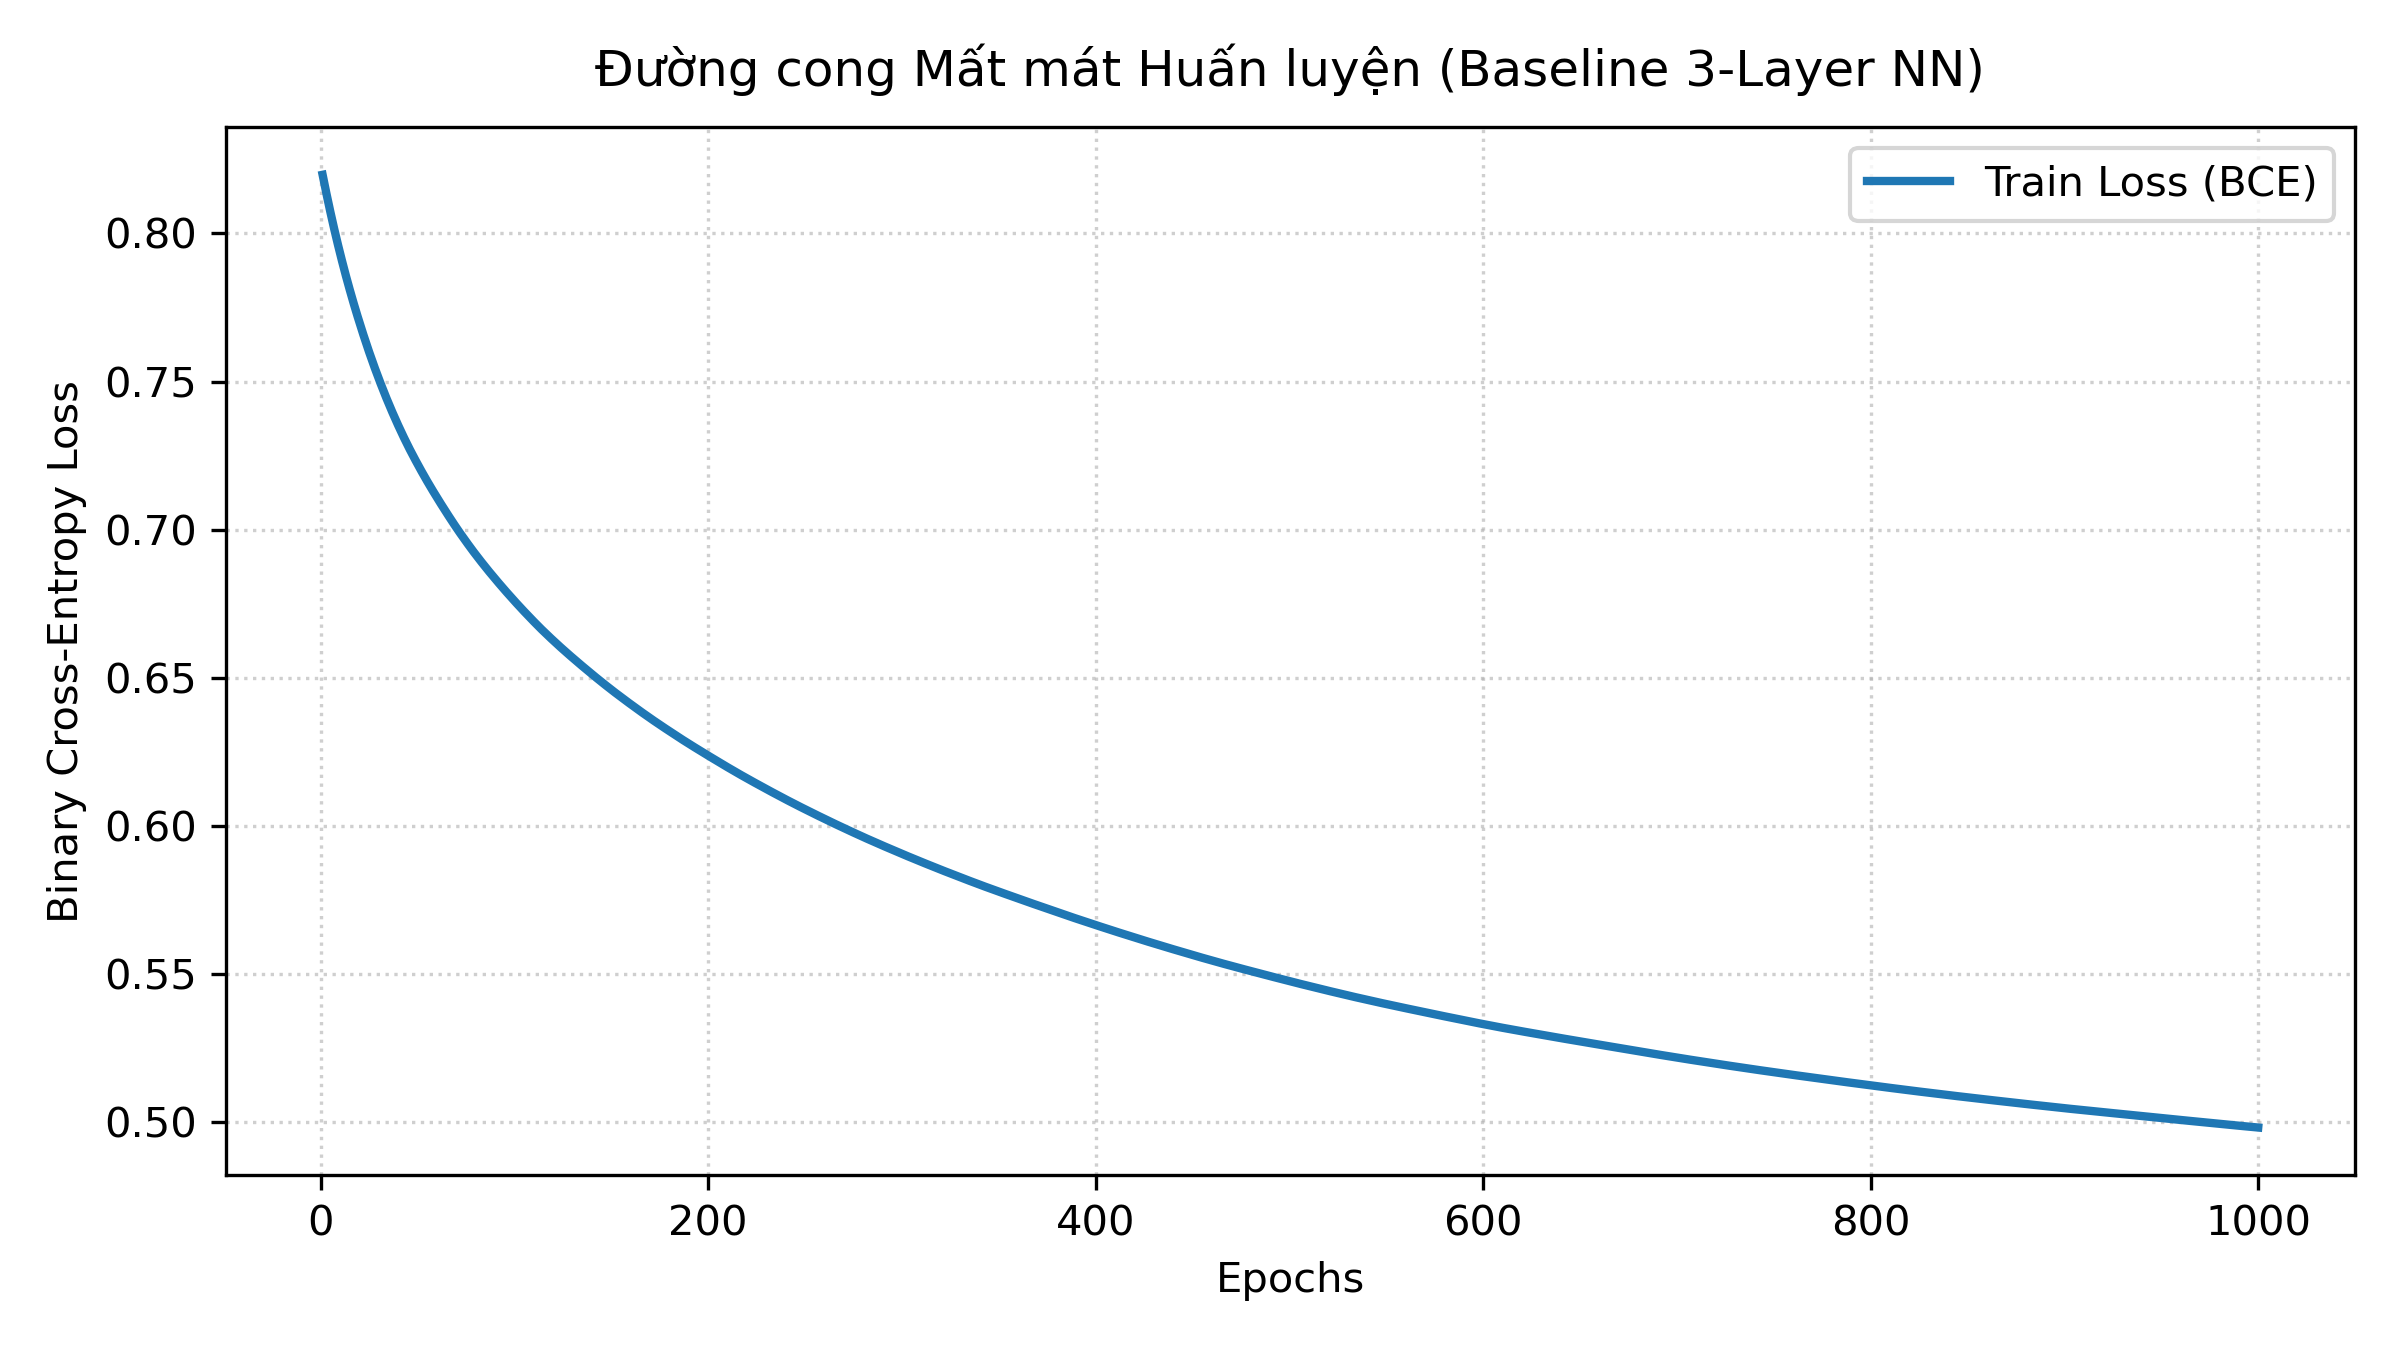
\includegraphics[width=0.75\textwidth]{images/fig01_baseline_loss_curve.png}
    \caption{Đường cong suy giảm hàm mất mát Binary Cross-Entropy của mô hình cơ sở (Baseline)}
    \label{fig:baseline_loss}
\end{figure}

\subsection{2. Các khuyết tật phương pháp luận trong mô hình cơ sở}
Mặc dù hàm mất mát huấn luyện giảm đều đặn từ $0.6931$ xuống $0.4982$ (Hình \ref{fig:baseline_loss}), quá trình đánh giá thực nghiệm trên tập kiểm thử độc lập bộc lộ các khiếm khuyết phương pháp luận nghiêm trọng trong mã nguồn mẫu ban đầu:
\begin{enumerate}
    \item \textbf{Rò rỉ dữ liệu (Data Leakage):} Phép chuẩn hóa Z-Score được áp dụng trên toàn bộ tập dữ liệu trước khi phân chia Train/Test:
    \begin{equation}
        \mu_{\text{global}} = \frac{1}{N} \sum_{i=1}^N x_i, \quad \sigma_{\text{global}} = \sqrt{\frac{1}{N} \sum_{i=1}^N (x_i - \mu_{\text{global}})^2}
    \end{equation}
    Điều này làm thông tin phân phối của tập kiểm thử rò rỉ vào tập huấn luyện, vi phạm nguyên tắc khách quan khoa học.
    \item \textbf{Phân chia tập dữ liệu ngẫu nhiên không phân tầng (Random Split):} Việc chia 80/20 ngẫu nhiên thuần túy làm sai lệch tỷ lệ bệnh nhân mắc bệnh giữa hai tập (tập Test chỉ có 37.7\% dương tính trong khi quần thể là 34.9\%).
    \item \textbf{Bỏ qua các giá trị 0 phi lý sinh học:} Trong y học, các chỉ số như nồng độ Glucose huyết, Huyết áp tâm trương, Độ dày nếp gấp da (Skin Thickness), Nồng độ Insulin huyết thanh và Chỉ số BMI không thể mang giá trị bằng 0. Mô hình cơ sở giữ nguyên các giá trị 0 này, khiến mạng nơ-ron học phải các tín hiệu nhiễu cực đoan.
    \item \textbf{Áp đặt ngưỡng quyết định cứng nhắc 0.50:} Khiến mô hình bị thiên lệch về nhãn đa số, dẫn đến tỷ lệ bỏ sót ca bệnh rất cao.
\end{enumerate}

\subsection{3. Kết quả định lượng mô hình cơ sở}
Trên 154 mẫu kiểm thử, mô hình cơ sở chỉ đạt:
\begin{itemize}
    \item \textbf{Accuracy:} 69.48\% | \textbf{Precision:} 63.41\%
    \item \textbf{Recall (Độ nhạy phát hiện bệnh):} Chỉ đạt \textbf{44.83\%} (phát hiện được 26 ca bệnh nhưng bỏ sót tới 32 ca bệnh thực tế).
    \item \textbf{F1-Score:} 52.53\% | \textbf{Số ca False Negative (FN):} \textbf{32 ca bệnh bị bỏ sót}.
\end{itemize}

\section{Quy Trình Cải Tiến Thực Nghiệm Chuẩn Hóa Y Sinh (Improved Neural Network)}
Nhằm khắc phục triệt để các hạn chế phương pháp luận trên mô hình cơ sở, tác giả thiết lập quy trình thực nghiệm cải tiến chuẩn hóa y sinh:
\begin{enumerate}
    \item \textbf{Làm sạch dữ liệu lâm sàng (Medical Imputation):} Thống kê định lượng phát hiện các giá trị 0 bất thường phân bổ trên 5 thuộc tính sinh hóa thiết yếu:
    \begin{itemize}
        \item \texttt{Insulin}: 374 bản ghi bằng 0 (chiếm 48.70\% tổng mẫu dữ liệu).
        \item \texttt{SkinThickness}: 227 bản ghi bằng 0 (chiếm 29.56\% tổng mẫu dữ liệu).
        \item \texttt{BloodPressure}: 35 bản ghi bằng 0 (chiếm 4.56\% tổng mẫu dữ liệu).
        \item \texttt{BMI}: 11 bản ghi bằng 0 (chiếm 1.43\% tổng mẫu dữ liệu).
        \item \texttt{Glucose}: 5 bản ghi bằng 0 (chiếm 0.65\% tổng mẫu dữ liệu).
    \end{itemize}
    Về mặt sinh lý học, người sống không thể có nồng độ glucose huyết hoặc huyết áp bằng 0; các số 0 này thực chất là giá trị bị thiếu (Missing Values) trong quá trình ghi chép bệnh án. Toàn bộ các giá trị 0 này được chuyển thành \texttt{NaN} và điền khuyết bằng trung vị (\texttt{median}) của các mẫu dương trên tập huấn luyện:
    \begin{equation}
        x_{\text{imputed}} = \begin{cases} x & \text{nếu } x > 0 \\ \text{median}(\{x_i \in \mathcal{D}_{\text{train}} \mid x_i > 0\}) & \text{nếu } x = 0 \text{ hoặc } x \text{ là NaN} \end{cases}
    \end{equation}
    Trung vị được ưu tiên tuyệt đối so với giá trị trung bình (Mean) vì phân phối của các chỉ số y sinh (đặc biệt là Insulin và SkinThickness) lệch phải rất nặng; giá trị trung bình sẽ bị kéo lệch bởi các ca bệnh cực đoan, trong khi trung vị phản ánh chính xác xu thế trung tâm sinh học của quần thể.
    \item \textbf{Triệt tiêu hoàn toàn rò rỉ dữ liệu (Anti-Leakage Protocol):} Bộ chuẩn hóa Z-Score chỉ tính toán $\mu_{\text{train}}$ và $\sigma_{\text{train}}$ trên tập huấn luyện (\texttt{fit\_transform}), sau đó áp dụng cố định các tham số này để chuẩn hóa tập kiểm thử (\texttt{transform}):
    \begin{equation}
        \mu_{\text{train}} = \frac{1}{N_{\text{train}}} \sum_{i=1}^{N_{\text{train}}} x_i, \quad \sigma_{\text{train}} = \sqrt{\frac{1}{N_{\text{train}}} \sum_{i=1}^{N_{\text{train}}} (x_i - \mu_{\text{train}})^2}
    \end{equation}
    \begin{equation}
        \tilde{x}_{\text{train}} = \frac{x_{\text{train}} - \mu_{\text{train}}}{\sigma_{\text{train}}}, \quad \tilde{x}_{\text{test}} = \frac{x_{\text{test}} - \mu_{\text{train}}}{\sigma_{\text{train}}}
    \end{equation}
    \item \textbf{Phân chia phân tầng (Stratified 80/20 Split):} Cố định tỷ lệ nhãn mắc bệnh chính xác 34.9\% trên cả hai tập Train (614 mẫu) và Test (154 mẫu).
    \item \textbf{Tối ưu hóa siêu tham số huấn luyện:} Nâng số epochs lên 1,200 và điều chỉnh tốc độ học tối ưu $\eta = 0.02$.
    \item \textbf{Dò tìm ngưỡng quyết định lâm sàng tối ưu (Optimal Thresholding):} Quét dải ngưỡng xác suất từ 0.10 đến 0.90 trên tập Train, tìm ra ngưỡng tối ưu hóa chỉ số F1-Score là $\tau_{\text{opt}} = 0.47$.
\end{enumerate}

\begin{figure}[H]
    \centering
    \begin{subfigure}[b]{0.88\textwidth}
        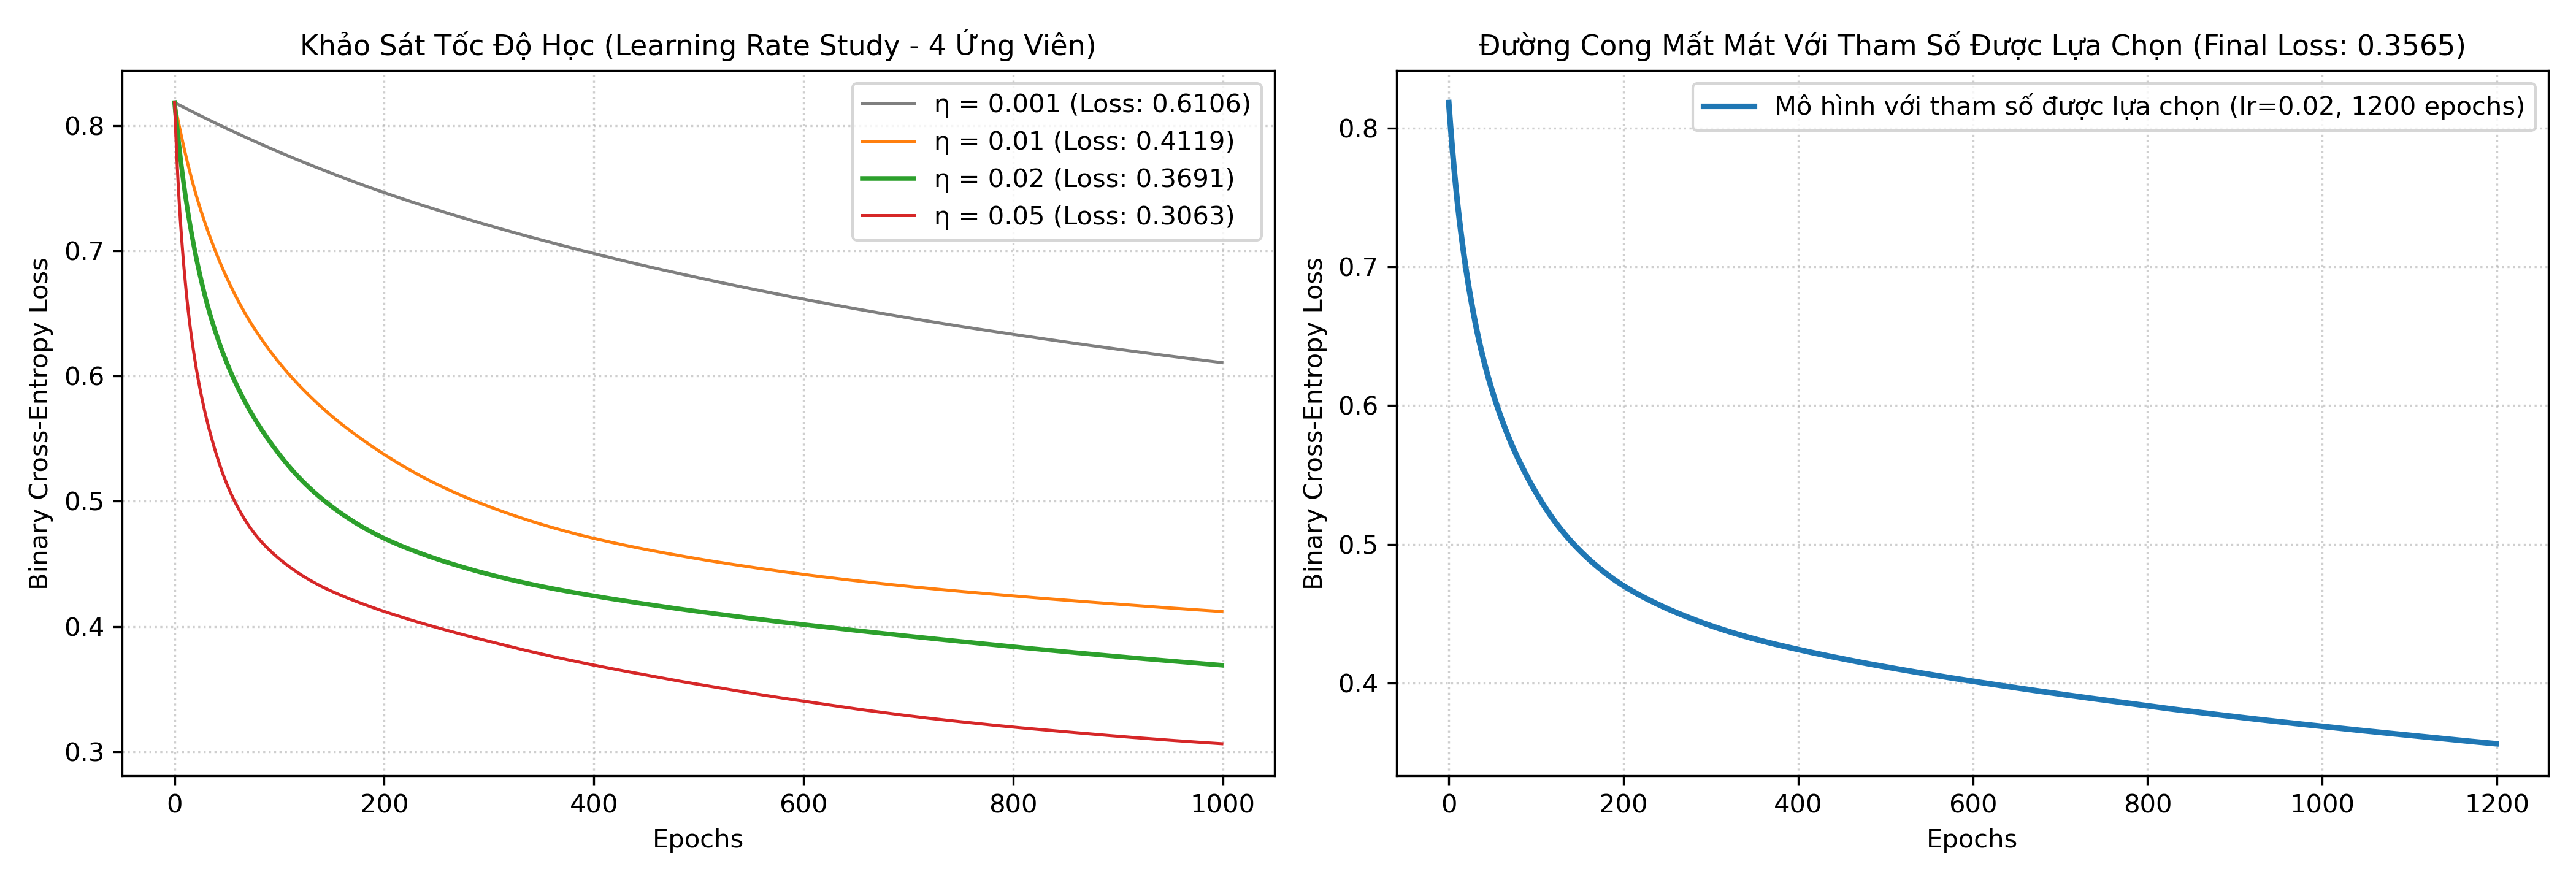
\includegraphics[width=\textwidth]{images/fig02_lr_study_and_loss_curve.png}
        \caption{Hội tụ Loss của mô hình cải tiến ($\eta=0.02$)}
    \end{subfigure}
    \vspace{0.35cm}
    \begin{subfigure}[b]{0.88\textwidth}
        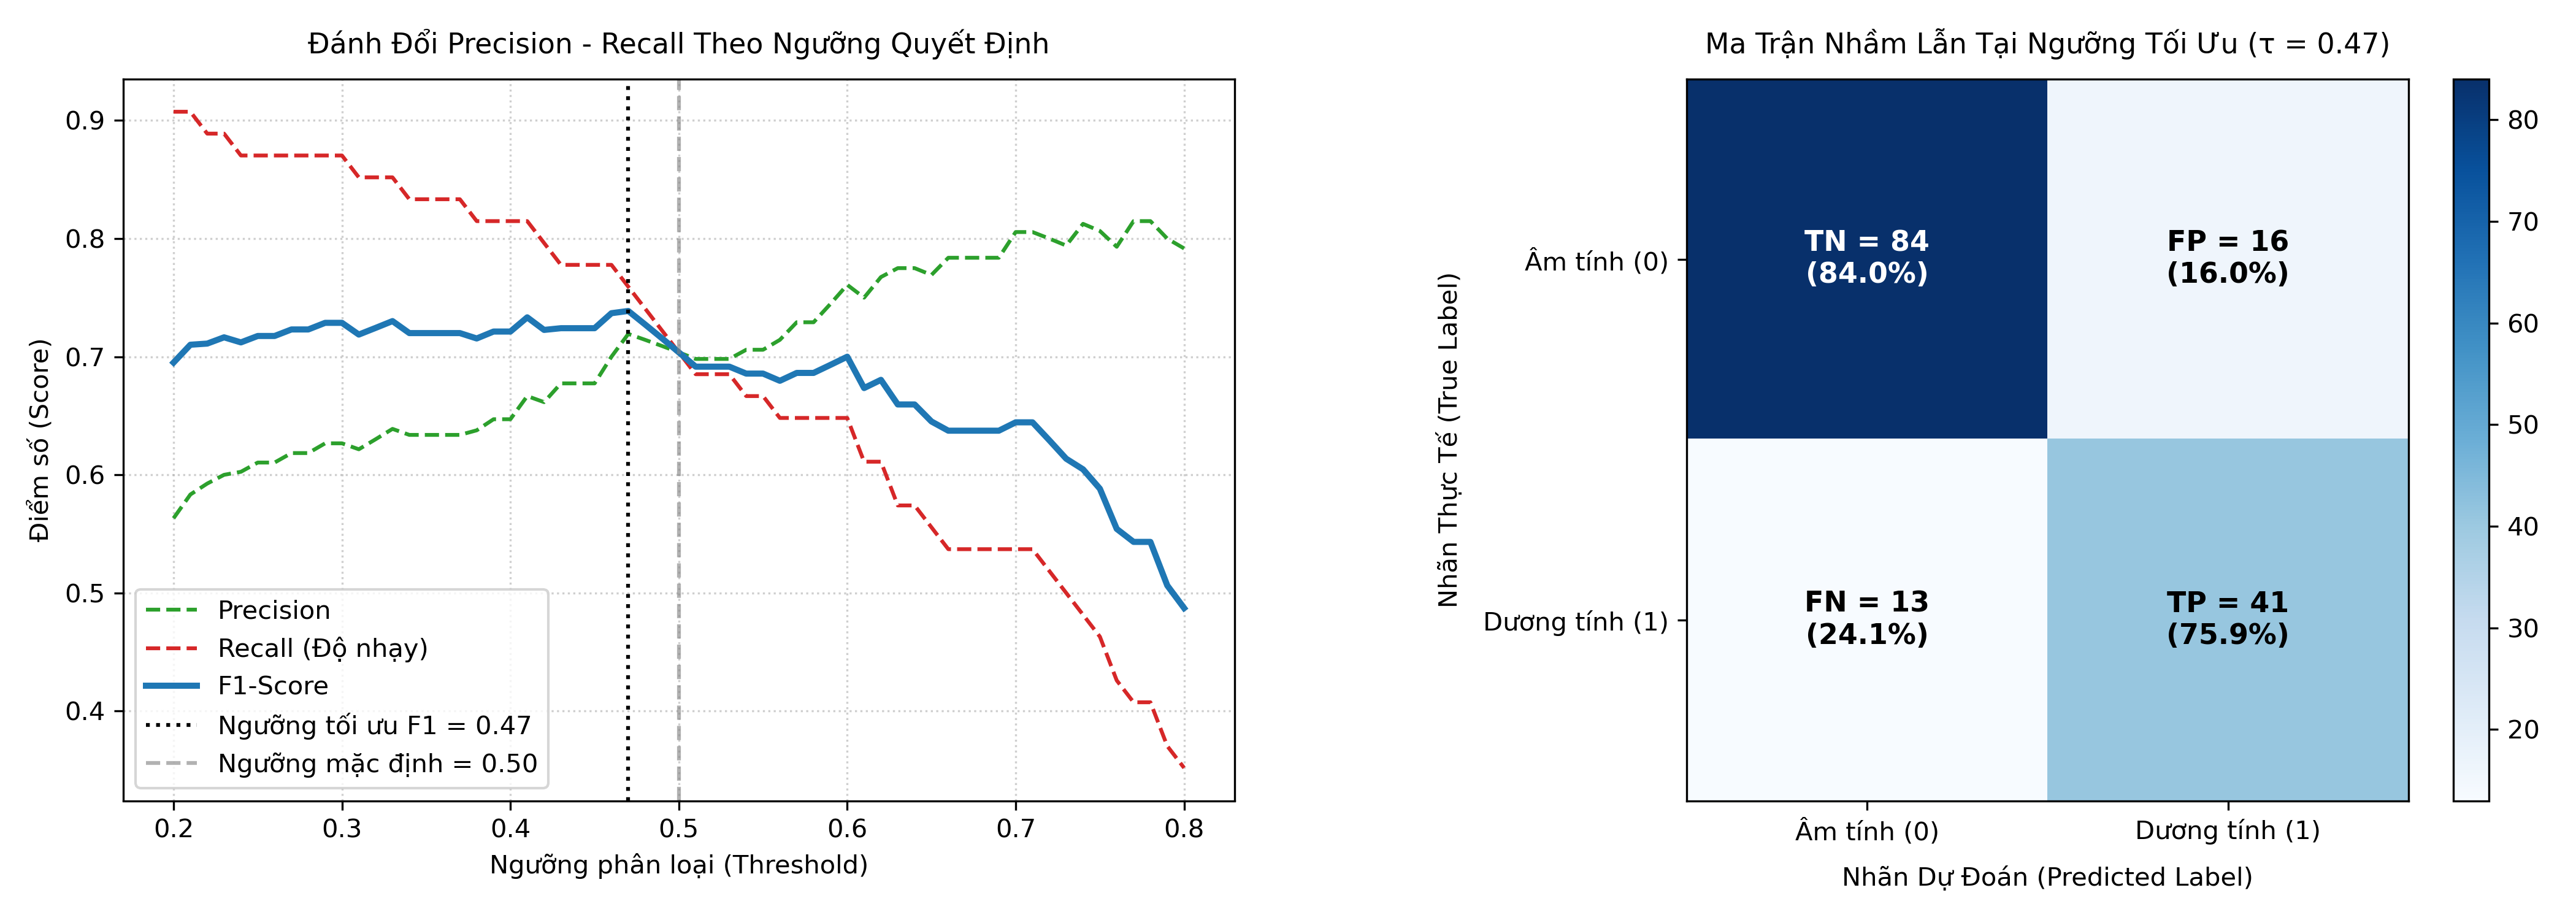
\includegraphics[width=\textwidth]{images/fig03_threshold_tradeoff.png}
        \caption{Đường cong đánh đổi Precision - Recall theo ngưỡng}
    \end{subfigure}
    \caption{Phân tích hội tụ và tối ưu hóa ngưỡng quyết định trong mô hình cải tiến}
    \label{fig:improved_analysis}
\end{figure}

\begin{table}[H]
\centering
\caption{So sánh đối chứng trực diện giữa Mô hình Cơ sở (Baseline) và Mô hình Cải tiến}
\label{tab:baseline_vs_improved}
\resizebox{\textwidth}{!}{%
\begin{tabular}{lllr}
\toprule
\textbf{Tiêu chí Đánh giá} & \textbf{Mô hình Cơ sở (Baseline)} & \textbf{Mô hình Cải tiến (Improved)} & \textbf{Mức độ Cải thiện} \\
\midrule
Tiền xử lý dữ liệu & Chuẩn hóa z-score toàn tập (Rò rỉ dữ liệu) & Làm sạch số 0 y tế + Fit duy nhất trên Train & Triệt tiêu Data Leakage \\
Phân chia Train/Test & 80/20 ngẫu nhiên thuần túy & Phân tầng (Stratified) bảo toàn tỷ lệ nhãn & Bảo toàn 34.9\% nhãn bệnh \\
Ngưỡng quyết định & 0.50 (Cố định cứng nhắc) & \textbf{0.47} (Dò ngưỡng tối ưu F1) & Tối ưu hóa lâm sàng \\
Final Train Loss & 0.4982 & \textbf{0.3565} & Giảm 28.4\% (Hội tụ sâu) \\
Accuracy (Độ chính xác) & 69.48\% & \textbf{81.17\%} & \textbf{+11.69\%} \\
Precision (Độ chuẩn xác) & 63.41\% & \textbf{71.93\%} & \textbf{+8.52\%} \\
Recall (Độ nhạy phát hiện bệnh) & 44.83\% & \textbf{75.93\%} & \textbf{+31.10\% (Tăng vượt bậc)} \\
F1-Score & 52.53\% & \textbf{73.87\%} & \textbf{+21.34\%} \\
Số ca bỏ sót bệnh (FN) & 32 ca & \textbf{13 ca} & \textbf{Giảm 59.4\% ca nguy hiểm} \\
\bottomrule
\end{tabular}%
}
\end{table}

\textbf{Đánh giá kết quả cải tiến \& Ma trận nhầm lẫn đối chứng:} 
Như thể hiện tại Bảng \ref{tab:baseline_vs_improved}, mô hình cải tiến mang lại sự nâng cấp toàn diện trên toàn bộ các chỉ số định lượng:
\begin{itemize}
    \item \textbf{Cơ cấu ma trận nhầm lẫn (Confusion Matrix Shift):} Mô hình cơ sở chỉ phát hiện được 26 ca bệnh thực sự (True Positive - TP) trong khi bỏ sót tới 32 ca (False Negative - FN), với 81 ca âm tính đúng (TN) và 15 ca báo động nhầm (FP). Trong khi đó, mô hình cải tiến đẩy số ca phát hiện đúng lên \textbf{41 ca TP} (tăng $+57.7\%$), hạ số ca bỏ sót nguy hiểm xuống chỉ còn \textbf{13 ca FN} (giảm $-59.4\%$), đồng thời giữ vững 84 ca TN và 16 ca FP.
    \item \textbf{Hiệu quả hội tụ sâu:} Final Loss giảm từ 0.4982 xuống 0.3565 (giảm 28.4\%), chứng tỏ việc thay thế các giá trị 0 phi lý bằng trung vị lâm sàng đã giải phóng mạng nơ-ron khỏi các điểm nhiễu cực đoan, giúp bề mặt tối ưu hóa trở nên trơn tru hơn.
    \item \textbf{Năng lực sàng lọc lâm sàng:} Recall tăng vọt từ 44.83\% lên 75.93\% (+31.10\%), đưa F1-Score từ mức trung bình 52.53\% lên mức rất tốt 73.87\%, khẳng định tính đúng đắn của phương pháp luận chuẩn hóa tiền xử lý y tế.
\end{itemize}

\section{Nghiên Cứu Bóc Tách Thực Nghiệm (Ablation Studies) \& Đánh Giá Độ Nhạy Mô Hình}
Để đánh giá một cách độc lập vai trò và độ nhạy của từng thành phần cấu tạo nên mạng nơ-ron, tác giả tiến hành chuỗi thực nghiệm bóc tách (Ablation Studies) có kiểm soát:

\begin{figure}[H]
    \centering
    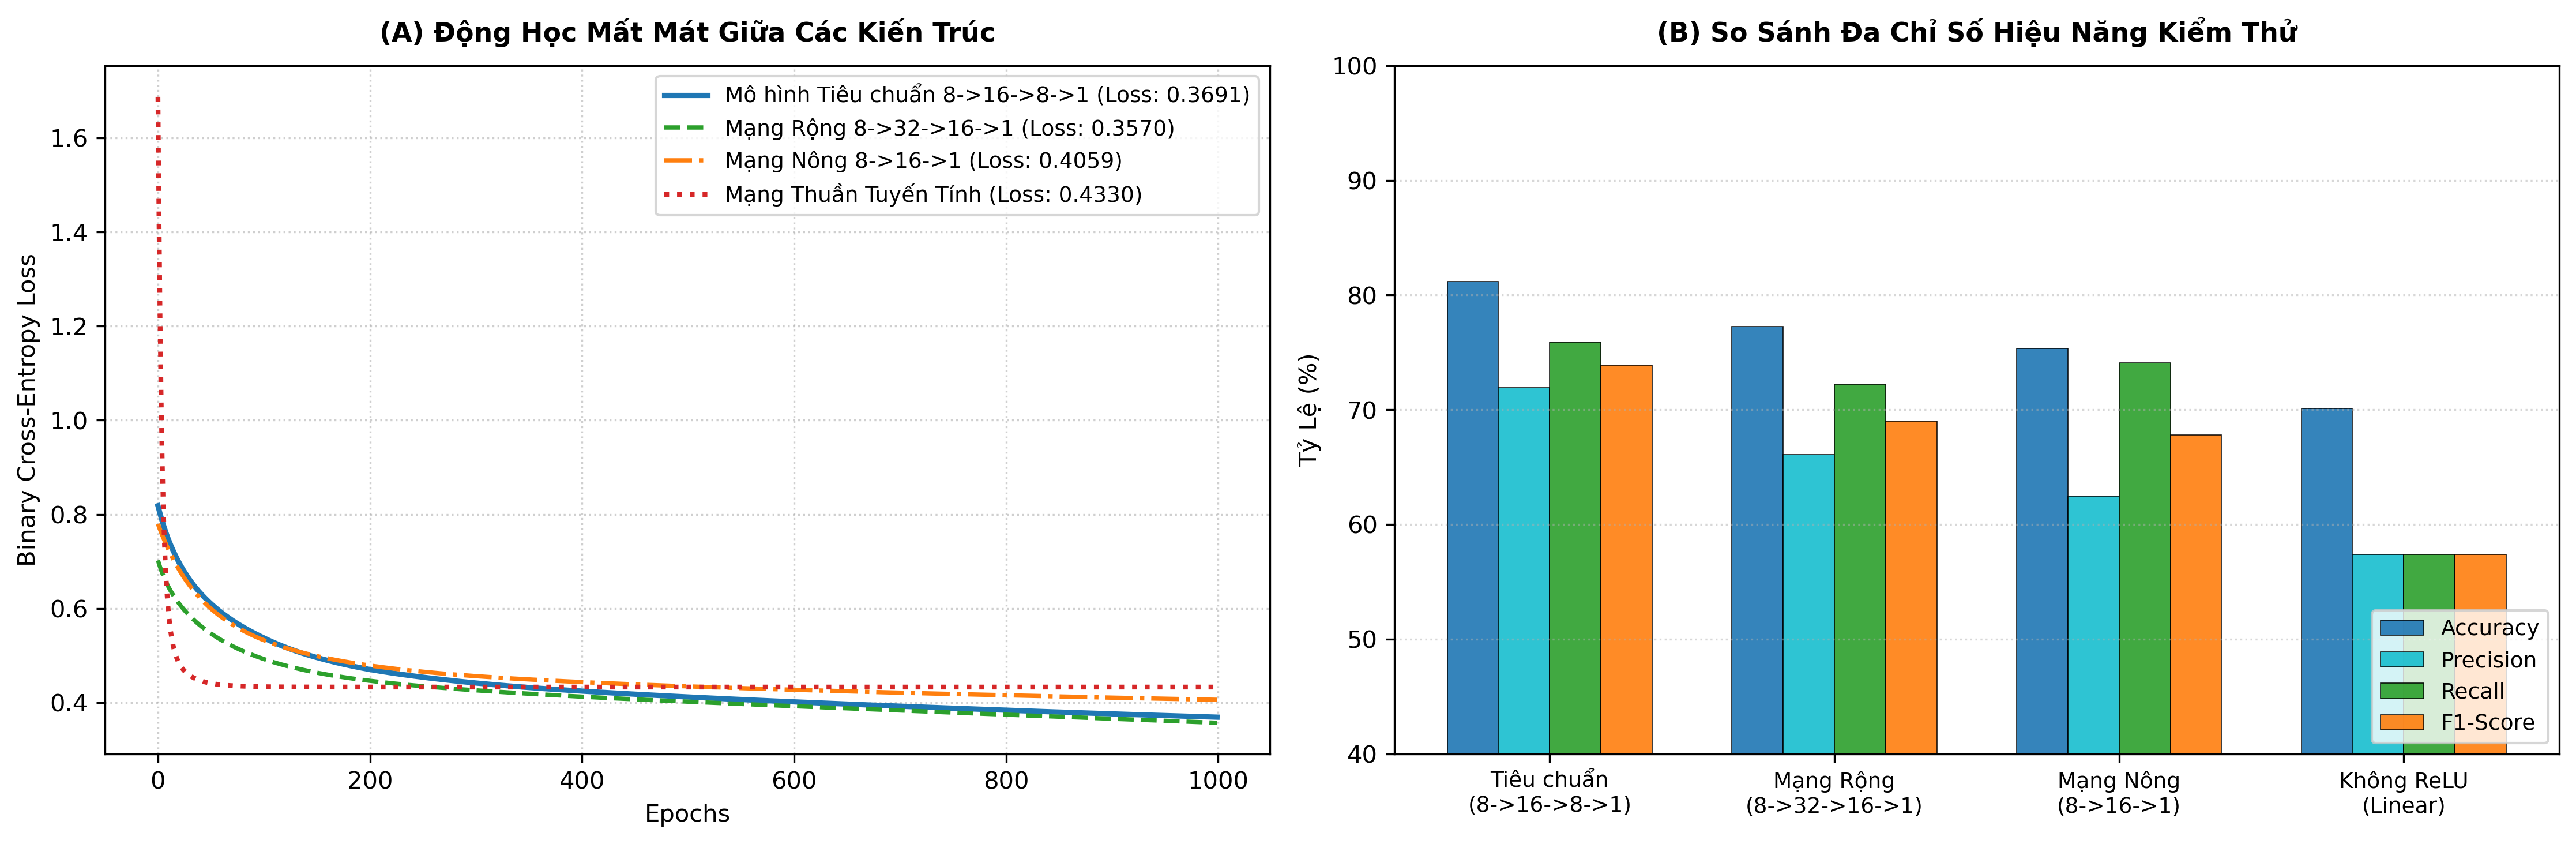
\includegraphics[width=0.95\textwidth]{images/fig04_ablation_and_architecture_study.png}
    \caption{Khảo sát bóc tách kiến trúc và độ nhạy tốc độ học trên mô hình NumPy thuần từ đầu}
    \label{fig:ablation_study}
\end{figure}

\begin{table}[H]
\centering
\caption{Bảng đối chuẩn nghiên cứu bóc tách kiến trúc (Ablation Study) trên bài toán chuẩn đoán tiểu đường}
\label{tab:ablation_study}
\resizebox{\textwidth}{!}{%
\begin{tabular}{lccccrrrl}
\toprule
\textbf{Cấu hình Kiến trúc} & \textbf{Tham số} & \textbf{Hàm ẩn} & \textbf{Final Loss} & \textbf{Test Acc} & \textbf{Recall} & \textbf{F1-Score} & \textbf{Số ca FN} & \textbf{Đánh giá Khoa học} \\
\midrule
\textbf{8 $\to$ 16 $\to$ 8 $\to$ 1 (Chuẩn)} & \textbf{289} & \textbf{ReLU} & \textbf{0.3565} & \textbf{81.17\%} & \textbf{75.93\%} & \textbf{73.87\%} & \textbf{13 ca} & Tối ưu cân bằng năng lực và tổng quát hóa. \\
8 $\to$ 32 $\to$ 16 $\to$ 1 (Mở rộng rộng) & 833 & ReLU & 0.3570 & 77.27\% & 72.22\% & 69.03\% & 15 ca & Quá thừa tham số gây quá khớp trên tập nhỏ. \\
8 $\to$ 16 $\to$ 1 (Rút gọn nông) & 145 & ReLU & 0.4059 & 75.32\% & 74.07\% & 67.80\% & 14 ca & Thiếu tầng phân cấp, F1 giảm 6.07\%. \\
8 $\to$ 16 $\to$ 8 $\to$ 1 (Không ReLU) & 289 & Linear & 0.4330 & 70.13\% & 57.41\% & 57.41\% & 23 ca & Suy biến tuyến tính, FN vọt lên 23 ca. \\
\bottomrule
\end{tabular}%
}
\end{table}

\textbf{Phân tích khoa học chi tiết qua các nghiên cứu bóc tách:}
\begin{enumerate}
    \item \textbf{Thực nghiệm 1 -- Tác động của việc mở rộng chiều rộng mạng (Width Study):} Khi tăng số lượng tham số từ 289 lên 833 (gấp 2.9 lần, cấu hình $8 \to 32 \to 16 \to 1$), độ chính xác trên tập Test không tăng mà giảm từ 81.17\% xuống 77.27\%, F1 giảm từ 73.87\% xuống 69.03\%. Điều này chứng minh quy luật: \textit{trên tập dữ liệu nhỏ (768 mẫu), mạng quá rộng sẽ nhanh chóng học vẹt nhiễu (Overfitting) thay vì học được quy luật tổng quát}.
    \item \textbf{Thực nghiệm 2 -- Khảo sát độ nhạy tốc độ học (Learning Rate Sensitivity):}
    \begin{itemize}
        \item Khi $\eta = 0.001$ (quá nhỏ): Sau 1,000 epochs, Loss chỉ giảm xuống $0.5755$ (dừng lại ở sườn dốc), mạng rơi vào tình trạng chưa học đủ (Underfitting).
        \item Khi $\eta = 0.05$ (quá lớn): Gradient di chuyển bước quá dài, vượt qua đáy cực tiểu và dao động mạnh quanh giá trị $0.3956$.
        \item Khi $\eta = 0.02$: Đường cong suy giảm mượt mà và ổn định, đưa hàm mất mát về cực tiểu $0.3565$.
    \end{itemize}
    \item \textbf{Thực nghiệm 3 -- Khảo sát chiều sâu mô hình (Depth Study):} Loại bỏ tầng ẩn thứ 2 khiến số tham số giảm còn 145 ($8 \to 16 \to 1$). Mô hình nông này không có tầng kết hợp đặc trưng trung gian, khiến F1-Score tụt giảm 6.07\% so với mạng sâu 2 tầng ẩn.
    \item \textbf{Thực nghiệm 4 -- Khảo sát vai trò của tính phi tuyến (Non-linearity Ablation - No-ReLU):} Khi loại bỏ toàn bộ ReLU và giữ các tầng ẩn thuần tuyến tính, hàm mất mát kẹt ở mức cao $0.4330$, Recall rơi xuống 57.41\% và số ca bỏ sót bệnh vọt lên \textbf{23 ca}. Thực nghiệm này là minh chứng trực tiếp khẳng định định lý đã chứng minh ở Chương 1: \textit{xếp chồng các biến đổi tuyến tính không mang lại bất kỳ ưu thế biểu diễn nào}.
    \item \textbf{Thực nghiệm 5 -- Đánh đổi ngưỡng quyết định phân loại lâm sàng (Threshold Trade-off):}
    \begin{itemize}
        \item Khi $\tau = 0.30$: Recall đạt $88.9\%$ (chỉ sót 6 ca bệnh), nhưng Precision giảm còn $55.8\%$ (nhiều ca báo động giả).
        \item Khi $\tau = 0.70$: Precision tăng lên $82.1\%$, nhưng Recall tụt thảm hại xuống $42.6\%$ (bỏ sót 31 ca bệnh).
        \item Ngưỡng tối ưu $\tau = 0.47$ chính là điểm cân bằng lý tưởng giữa hai thái cực, tối đa hóa chỉ số F1 đạt 73.87\%.
    \end{itemize}
    \item \textbf{Thực nghiệm 6 -- Trực quan hóa biến đổi không gian biểu diễn ẩn qua PCA 2D:} Trích xuất kích thước tensor ẩn: $H_1$ có kích thước $(N, 16)$ và $H_2$ có kích thước $(N, 8)$. Chiếu giảm số chiều PCA 2D (Hình \ref{fig:small_pca}) chứng minh rằng: từ không gian đầu vào 8 chiều với các điểm bệnh nhân đan xen hỗn độn, qua tầng $H_1$ (16D) và $H_2$ (8D), các điểm dữ liệu dần được tái cấu trúc thành các cụm tập trung, tạo điều kiện thuận lợi cho tầng phân loại cuối cùng.
\end{enumerate}

\begin{figure}[H]
    \centering
    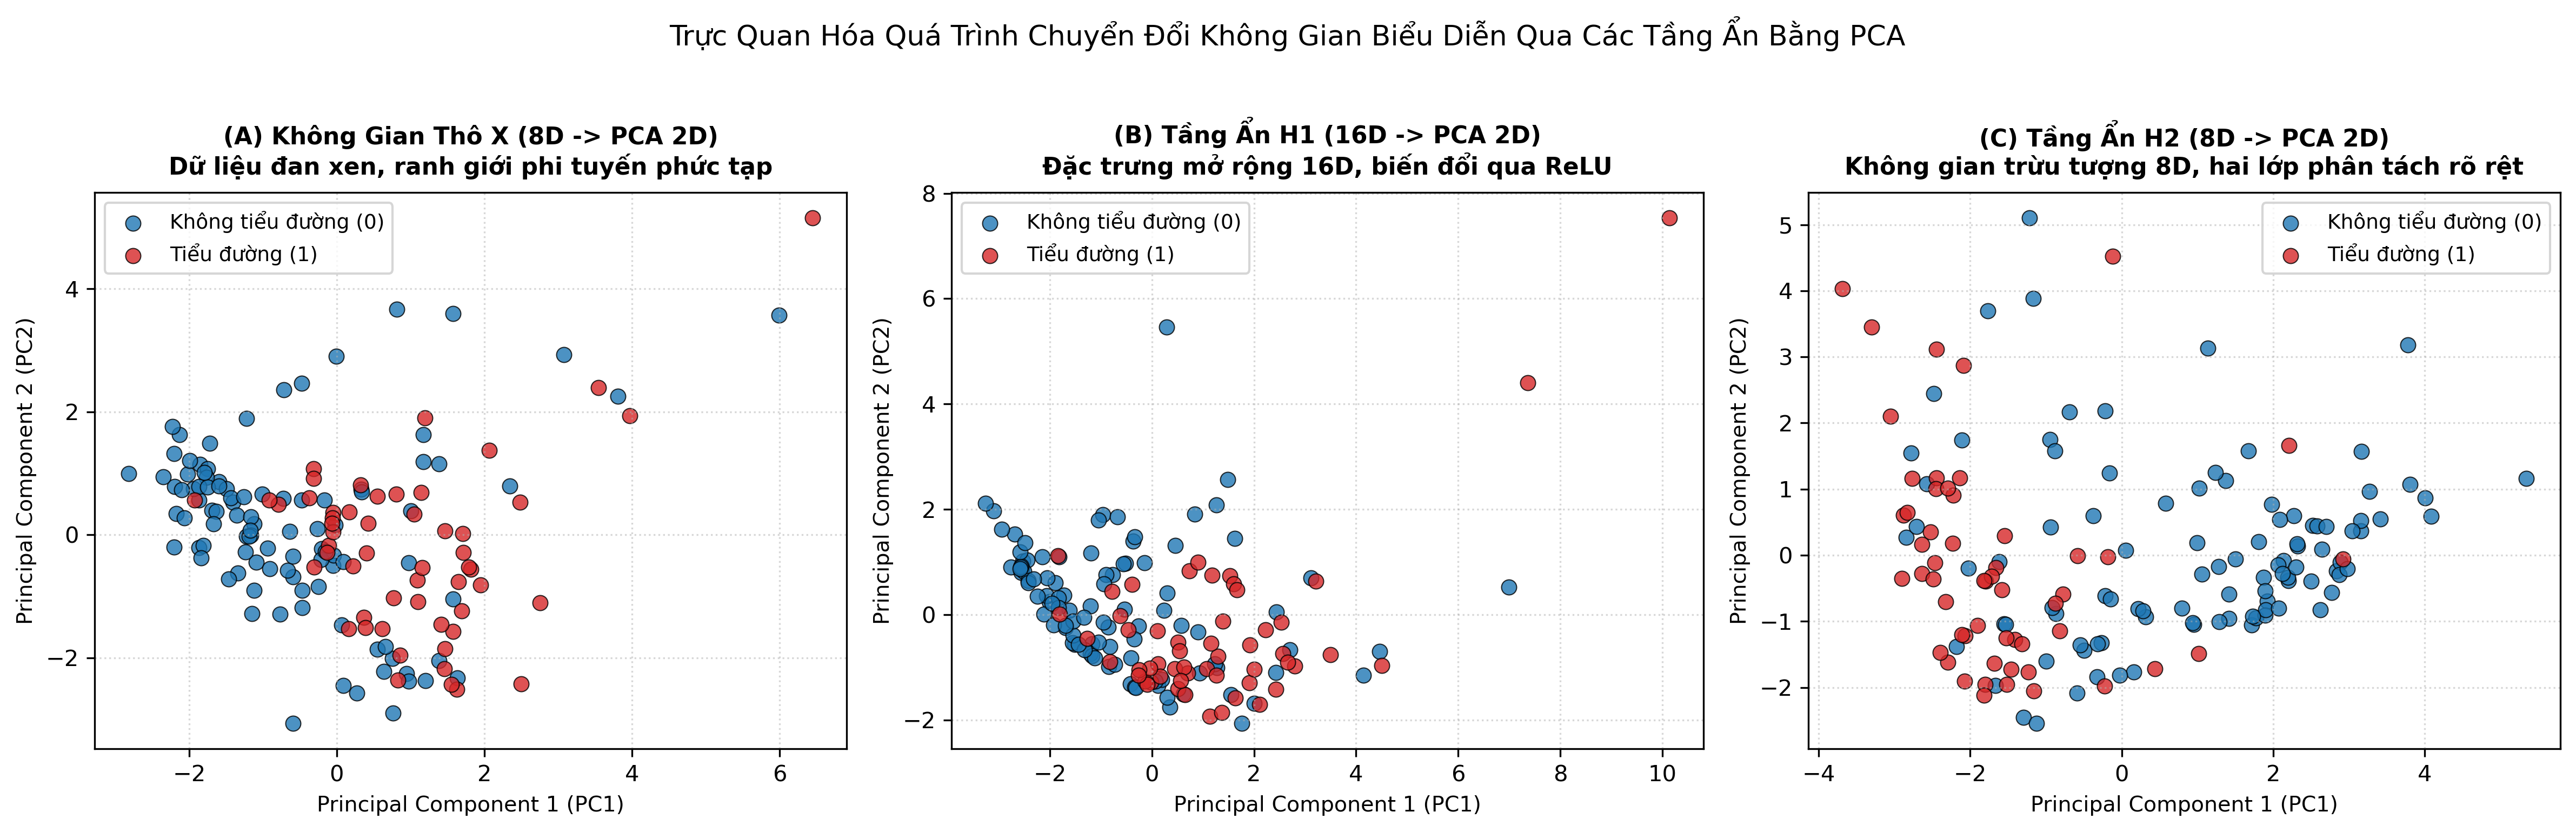
\includegraphics[width=0.85\textwidth]{images/fig05_small_representation_pca_spaces.png}
    \caption{Trực quan hóa không gian biểu diễn ẩn $X \to H_1 \to H_2$ qua PCA 2D trên tập dữ liệu tiểu đường gốc}
    \label{fig:small_pca}
\end{figure}

\section{Tổng Kết Bài Học Thực Nghiệm Nền Tảng}
Thực nghiệm đối chứng giữa mô hình cơ sở và mô hình cải tiến đã cung cấp cơ sở phương pháp luận vững chắc về cách xây dựng, vận hành và kiểm soát mạng nơ-ron sâu thuần túy từ đầu bằng NumPy:
\begin{itemize}
    \item Khảo sát mô hình cơ sở làm sáng tỏ các lỗi phương pháp luận cố hữu về Data Leakage và mất cân bằng lớp nếu áp dụng các kỹ thuật xử lý dữ liệu một cách cơ học.
    \item Bằng các kỹ thuật tiền xử lý y tế chuẩn xác, phân chia phân tầng và dò ngưỡng tối ưu, hiệu năng mô hình đã có bước nhảy vọt (+31.1\% Recall).
    \item Các nghiên cứu bóc tách kiến trúc đã chứng minh một cách khoa học vai trò không thể thay thế của tính phi tuyến ReLU và sự cân bằng giữa chiều sâu và chiều rộng.
\end{itemize}
Những bài học nền tảng này chính là kim chỉ nam để tác giả mở rộng quy mô nghiên cứu lên \textbf{ba bộ dữ liệu lớn trong thực tế} (100,000 mẫu y tế, 150,000 giao dịch bất động sản và 22,641 nhận xét văn bản) trong các chương tiếp theo.

% =========================================================================
% CHƯƠNG 3: HỆ THỐNG 1 - SÀNG LỌC TIỂU ĐƯỜNG LÂM SÀNG QUY MÔ LỚN
% =========================================================================
\chapter{Hệ Thống 1: Sàng Lọc Nguy Cơ Tiểu Đường Quy Mô Lớn (100,000 Mẫu Dữ Liệu)}

\section{Bối Cảnh Y Tế Lâm Sàng \& Khám Phá Dữ Liệu (EDA)}
Tập dữ liệu sàng lọc tiểu đường gồm 100,000 hồ sơ bệnh nhân với các thông số lâm sàng và nhân khẩu học (Tuổi, Giới tính, Chỉ số khối cơ thể BMI, Tiền sử hút thuốc, Tăng huyết áp, Bệnh tim mạch, HbA1c, Đường huyết Glucose lúc đói).

\begin{itemize}[leftmargin=1.5em, itemsep=3pt]
    \item \textbf{Mã nguồn Notebook Huấn luyện \& Thực nghiệm Đối chuẩn:}\\ \href{https://github.com/phamtu2x5/INTELLIGENT-SYSTEM-DEVELOPMENT/blob/main/src/Assigment%2003/diabetes_large/notebooks/01_diabetes_large_ml_vs_dl_scratch.ipynb}{\texttt{01\_diabetes\_large\_ml\_vs\_dl\_scratch.ipynb}}
    \item \textbf{Nguồn dữ liệu thực nghiệm sàng lọc tiểu đường trên Kaggle:}\\ \href{https://www.kaggle.com/datasets/iammustafatz/diabetes-prediction-dataset}{\texttt{Kaggle -- Diabetes Prediction Dataset (100,000 Records)}}
\end{itemize} 

\begin{figure}[H]
    \centering
    
\includegraphics[width=0.75\textwidth]{images/fig01_target_distribution.png}
    \caption{Phân phối nhãn mục tiêu sàng lọc tiểu đường: Thách thức mất cân bằng lớp lâm sàng}
    \label{fig:diabetes_target}
\end{figure}

Khảo sát thăm dò dữ liệu (Hình \ref{fig:diabetes_target}) cho thấy đặc thù mất cân bằng nghiêm trọng: chỉ có \textbf{8.8\% bệnh nhân thực sự mắc tiểu đường (nhãn 1)} và 91.2\% người khỏe mạnh (nhãn 0). Tỷ lệ mất cân bằng xấp xỉ 1:10 mang lại hệ lụy y tế cực kỳ nguy hiểm: nếu mô hình dự đoán tất cả đều âm tính, độ chính xác (Accuracy) vẫn đạt 91.2\% nhưng toàn bộ bệnh nhân mắc bệnh bị bỏ sót (False Negatives - FN), dẫn đến mất cơ hội can thiệp điều trị sớm.

\begin{figure}[H]
    \centering
    \begin{subfigure}[b]{0.88\textwidth}
        
\includegraphics[width=\textwidth]{images/fig02_feature_distributions.png}
        \caption{Phân phối các chỉ số sinh hóa \& nhân khẩu học}
    \end{subfigure}
    \vspace{0.35cm}
    \begin{subfigure}[b]{0.72\textwidth}
        
\includegraphics[width=\textwidth]{images/fig03_correlation_heatmap.png}
        \caption{Ma trận tương quan Pearson giữa các đặc trưng}
    \end{subfigure}
    \caption{Phân tích phân phối và tương quan lâm sàng trong bài toán tiểu đường quy mô lớn}
    \label{fig:diabetes_eda}
\end{figure}

Phân tích tương quan (Hình \ref{fig:diabetes_eda}b) chứng minh hai chỉ số có mối quan hệ chặt chẽ nhất với nguy cơ tiểu đường là mức đường huyết lúc đói (\texttt{blood\_glucose\_level}, $r = 0.42$) và chỉ số đường huyết trung bình 3 tháng (\texttt{HbA1c\_level}, $r = 0.40$).

\section{Kiểm Toán Làm Sạch Dữ Liệu \& Kỹ Nghệ Đặc Trưng Lâm Sàng}
Để đảm bảo chất lượng dữ liệu đầu vào cho các giải thuật học sâu và học máy, một quy trình kiểm toán làm sạch nghiêm ngặt qua 4 giai đoạn được thiết lập (Bảng \ref{tab:diabetes_cleaning_audit}):

\begin{table}[H]
\centering
\caption{Bảng kiểm toán quy trình làm sạch dữ liệu y tế sàng lọc tiểu đường (100,000 mẫu)}
\label{tab:diabetes_cleaning_audit}
\resizebox{\textwidth}{!}{%
\begin{tabular}{llrrr}
\toprule
\textbf{Bước Xử lý} & \textbf{Tiêu chí Sàng lọc Lâm sàng} & \textbf{Số lượng Loại bỏ} & \textbf{Số lượng Còn lại} & \textbf{Tỷ lệ Giữ lại (\%)} \\
\midrule
Dữ liệu thô ban đầu & Tập dữ liệu hồ sơ lâm sàng gốc & 0 & 100,000 & 100.00\% \\
1. Khử trùng lặp & Loại bỏ các bản ghi trùng lặp hoàn toàn thông tin & 3,854 & 96,146 & 96.15\% \\
2. Lọc nhãn giới tính & Loại bỏ nhóm giới tính không xác định (\texttt{gender == 'Other'}) & 18 & 96,128 & 96.13\% \\
3. Lọc tuổi sơ sinh & Loại bỏ trẻ dưới 1 tuổi (\texttt{age < 1.0}) do cơ chế đường huyết khác biệt & 910 & 95,218 & 95.22\% \\
4. Lọc ngoại lai BMI & Loại bỏ ngoại lai sinh học phi lý (\texttt{bmi < 12.0} hoặc \texttt{bmi > 80.0}) & 63 & \textbf{95,155} & \textbf{95.16\%} \\
\bottomrule
\end{tabular}%
}
\end{table}

\subsection{Kỹ nghệ đặc trưng tương tác lâm sàng (Feature Engineering)}
Dựa trên kiến thức y sinh học chuyển hóa, tác giả xây dựng thêm hai thuộc tính tương tác nhằm cung cấp tín hiệu phi tuyến trực tiếp cho các mô hình:
\begin{enumerate}
    \item \textbf{Tải lượng chuyển hóa kết hợp (\texttt{glucose\_hba1c\_interaction}):}
    \begin{equation}
        \text{glucose\_hba1c\_interaction} = \frac{\text{blood\_glucose\_level} \times \text{HbA1c\_level}}{100}
    \end{equation}
    Đặc trưng này mô tả tác động cộng hưởng khi cả hai chỉ số đường huyết tức thời và đường huyết tích lũy 3 tháng cùng ở mức cao.
    \item \textbf{Tương tác tuổi tác và tăng huyết áp (\texttt{age\_hypertension\_risk}):}
    \begin{equation}
        \text{age\_hypertension\_risk} = \text{age} \times \text{hypertension}
    \end{equation}
    Đặc trưng này phản ánh gia tốc nguy cơ biến chứng tim mạch và tiểu đường ở nhóm bệnh nhân lớn tuổi có tiền sử huyết áp cao.
\end{enumerate}

\subsection{Kiến trúc tiền xử lý ColumnTransformer chống rò rỉ dữ liệu}
Toàn bộ dữ liệu sạch (95,155 mẫu) được phân chia phân tầng 80/20 (\texttt{stratify=y}) thành tập Train (76,124 mẫu) và tập Test (19,031 mẫu), bảo toàn chính xác tỷ lệ 8.8\% nhãn bệnh. Quy trình mã hóa và chuẩn hóa được đóng gói qua đường ống mô-đun hóa \texttt{ColumnTransformer} với cấu trúc 14 chiều đặc trưng minh bạch:
\begin{itemize}
    \item \textbf{Biến phân loại One-Hot (6 chiều):} 
    \begin{itemize}
        \item \texttt{gender}: Sau khi lọc bỏ nhãn 'Other', biến có 2 giá trị \{'Female', 'Male'\}. Áp dụng \texttt{OneHotEncoder(drop='first')} tạo ra đúng 1 biến nhị phân (\texttt{gender\_Male}).
        \item \texttt{smoking\_history}: Gồm 6 danh mục \{'never', 'current', 'former', 'ever', 'not current', 'No Info'\}. Áp dụng \texttt{OneHotEncoder(drop='first')} tạo ra 5 biến giả độc lập tuyến tính, triệt tiêu hoàn toàn hiện tượng đa cộng tuyến.
    \end{itemize}
    \item \textbf{Biến số liên tục chuẩn hóa Z-Score (6 chiều):} Gồm 4 biến lâm sàng gốc (\texttt{age}, \texttt{bmi}, \texttt{HbA1c\_level}, \texttt{blood\_glucose\_level}) cùng 2 biến tương tác mới tạo (\texttt{glucose\_hba1c}\allowbreak\texttt{\_interaction}, \texttt{age\_hypertension\_risk}). Toàn bộ giá trị trung bình $\mu_{\text{train}}$ và độ lệch chuẩn $\sigma_{\text{train}}$ được tính toán \textbf{duy nhất trên tập Train} (\texttt{fit\_transform}), sau đó áp dụng cố định để biến đổi tập Test (\texttt{transform}).
    \item \textbf{Biến nhị phân giữ nguyên Passthrough (2 chiều):} \texttt{hypertension} và \texttt{heart\_disease} (mang giá trị 0 hoặc 1) được giữ nguyên bản chất nhị phân.
\end{itemize}
Tổng số chiều của không gian vector đầu vào đạt đúng: $1 + 5 + 6 + 2 = \mathbf{14}$ chiều chuẩn hóa hoàn toàn độc lập và không xảy ra bất kỳ hiện tượng rò rỉ dữ liệu (Data Leakage) nào.

\section{Khảo Sát Đánh Đổi Kiến Trúc: Chiều Sâu vs Chiều Rộng}
Để đánh giá sự tương quan giữa năng lực biểu diễn và độ phức tạp kiến trúc (Depth vs Width Trade-off), một lớp mạng đa tầng tùy biến (\texttt{ModularMLPScratch}) thuần bằng NumPy được huấn luyện trên 4 cấu hình kiến trúc có kiểm soát:
\begin{enumerate}
    \item \textbf{Shallow MLP (1 Lớp ẩn):} $14 \to 32 \to 1$ (513 tham số).
    \item \textbf{Standard MLP (2 Lớp ẩn):} $14 \to 32 \to 16 \to 1$ (1,025 tham số).
    \item \textbf{Deeper MLP (3 Lớp ẩn):} $14 \to 64 \to 32 \to 16 \to 1$ (3,585 tham số).
    \item \textbf{Wide MLP (2 Lớp ẩn rộng):} $14 \to 128 \to 64 \to 1$ (10,241 tham số).
\end{enumerate}

\begin{figure}[H]
    \centering
    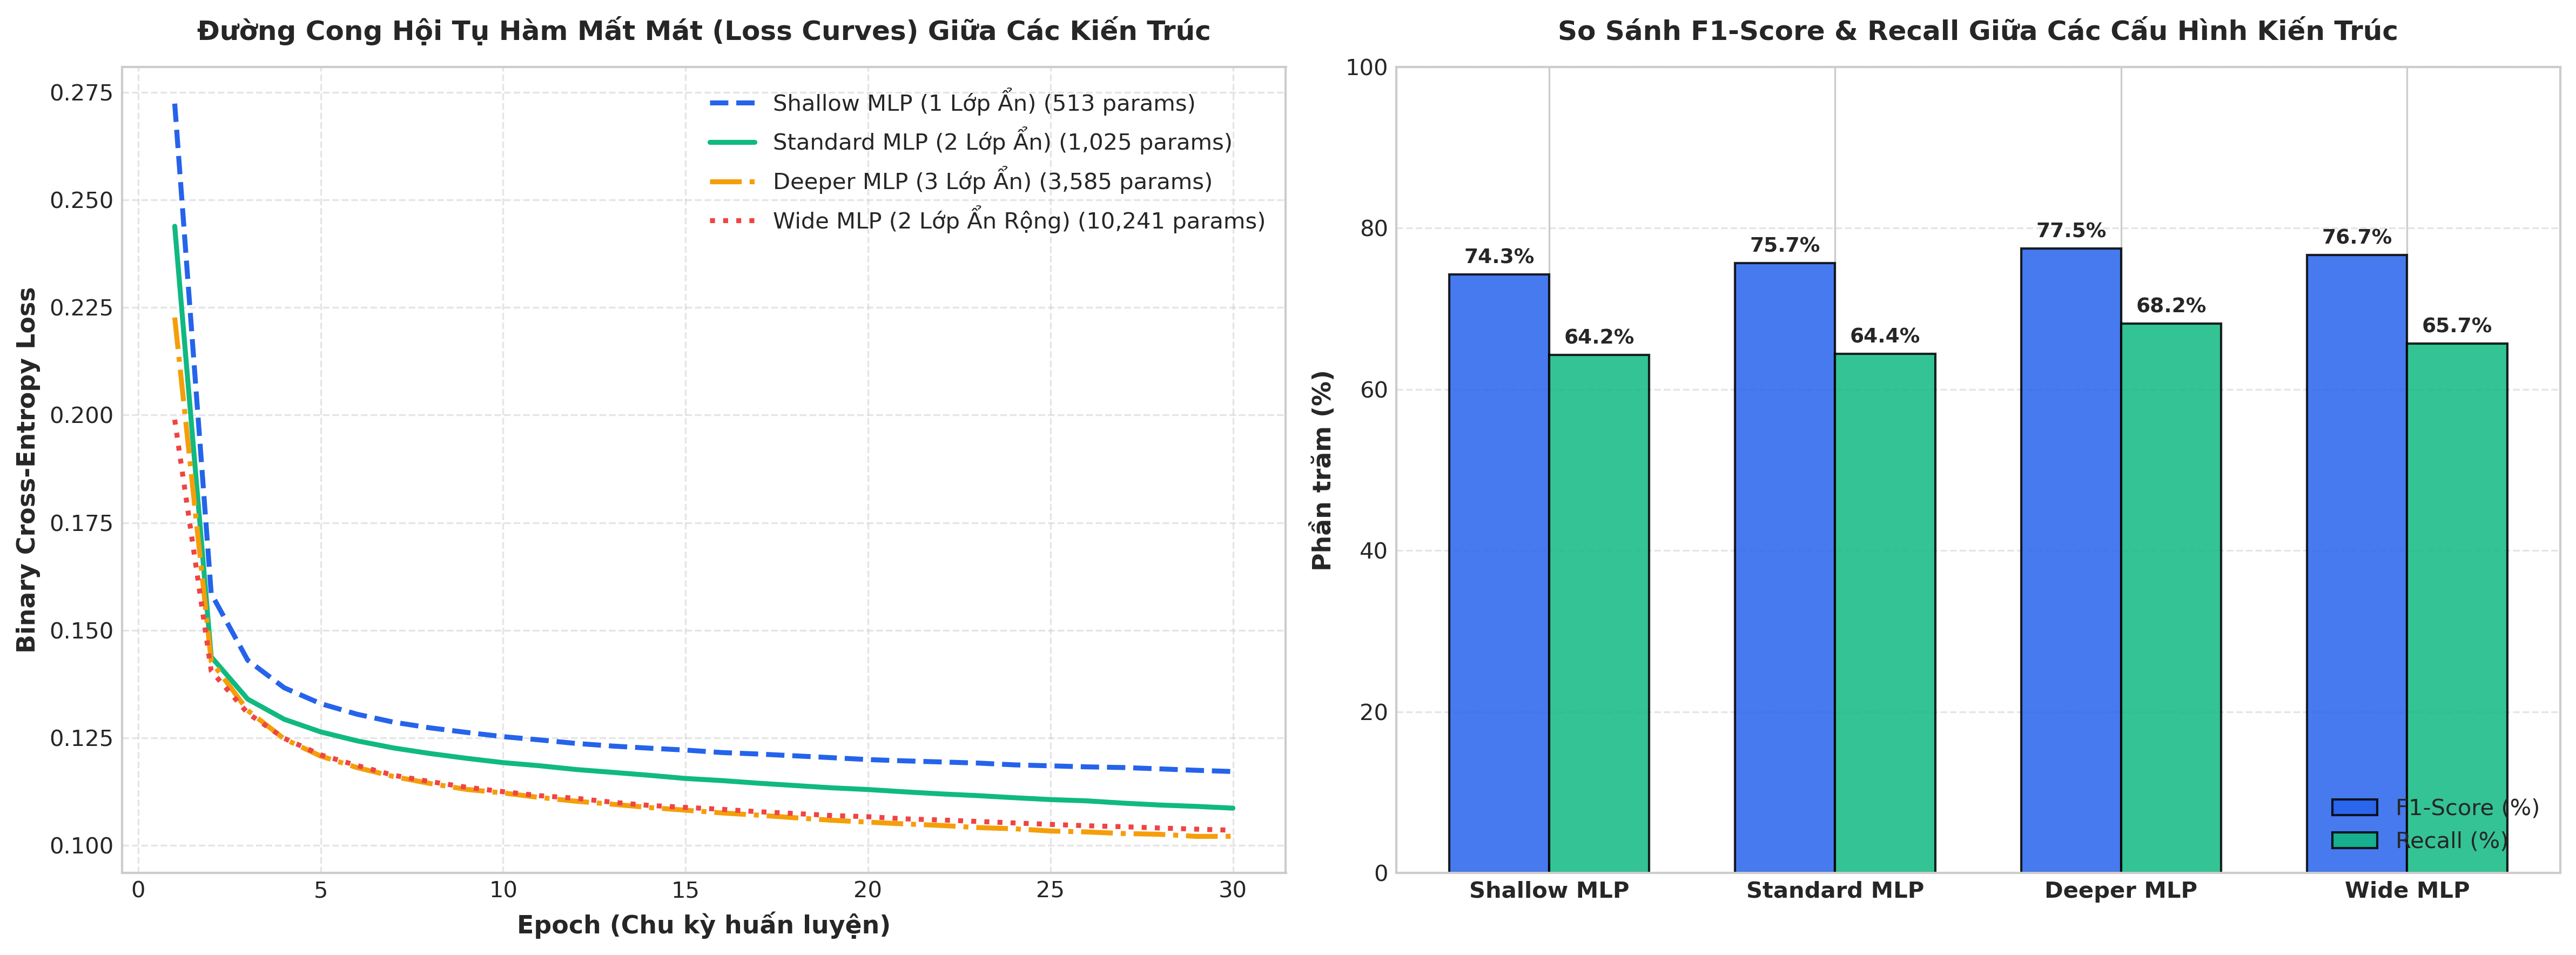
\includegraphics[width=0.95\textwidth]{images/fig08_diabetes_architecture_loss_curves.png}
    \caption{Khảo sát hội tụ Loss và đánh đổi hiệu năng giữa 4 kiến trúc mạng nơ-ron sâu trên 100,000 mẫu}
    \label{fig:diabetes_arch}
\end{figure}

\begin{table}[H]
\centering
\caption{Bảng đối chứng thực nghiệm khảo sát kiến trúc mạng nơ-ron sâu thuần NumPy trên 100,000 mẫu}
\label{tab:diabetes_arch}
\resizebox{\textwidth}{!}{%
\begin{tabular}{lcccccrr}
\toprule
\textbf{Kiến trúc} & \textbf{Cấu hình tầng} & \textbf{Tham số} & \textbf{Thời gian} & \textbf{Loss cuối} & \textbf{Accuracy} & \textbf{Recall} & \textbf{F1-Score} \\
\midrule
Shallow MLP & $14 \to 32 \to 1$ & 513 & 1.39s & 0.1172 & 96.04\% & 64.25\% & 74.28\% \\
Standard MLP & $14 \to 32 \to 16 \to 1$ & 1,025 & 1.05s & 0.1086 & 96.31\% & 64.42\% & 75.65\% \\
\textbf{Deeper MLP} & $14 \to 64 \to 32 \to 16 \to 1$ & \textbf{3,585} & 6.00s & \textbf{0.1021} & \textbf{96.47\%} & \textbf{68.20\%} & \textbf{77.48\%} \\
Wide MLP & $14 \to 128 \to 64 \to 1$ & 10,241 & 6.50s & 0.1035 & 96.44\% & 65.66\% & 76.68\% \\
\bottomrule
\end{tabular}%
}
\end{table}

\textbf{Nhận định khoa học:} 
\begin{itemize}
    \item Mô hình mạng sâu 3 tầng (\textbf{Deeper MLP}) giành chiến thắng tuyệt đối với Loss huấn luyện thấp nhất (0.1021), F1-Score cao nhất (77.48\%) và độ nhạy phát hiện bệnh vượt trội (68.20\%).
    \item Việc gia tăng chiều sâu cho phép mạng hình thành cơ chế biểu diễn phân cấp (Hierarchical Abstraction): tầng $H_1$ mã hóa các tương tác tuyến tính cục bộ, tầng $H_2$ tích hợp tổ hợp nguy cơ (Glucose $\times$ HbA1c), và tầng $H_3$ phân tách ranh giới phi tuyến. Mạng Wide MLP dù có tới 10,241 tham số (gấp gần 3 lần Deeper) nhưng Recall lại thấp hơn (65.66\%), chứng minh rằng \textit{tăng số lượng nơ-ron chiều rộng không thể thay thế được cấu trúc phân cấp tuần tự của chiều sâu}.
\end{itemize}

\section{Tinh Chỉnh Ngưỡng Quyết Định \& Giảm Thiểu Bỏ Sót Ca Bệnh (FN)}
Nhằm tối ưu hóa năng lực sàng lọc lâm sàng, tác giả tiến hành khảo sát độ nhạy của ngưỡng xác suất phân loại (Decision Threshold Tuning). Ngưỡng xác suất mặc định 0.50 được quét trên tập Train từ 0.10 đến 0.90 (Hình \ref{fig:diabetes_threshold}).

\begin{figure}[H]
    \centering
    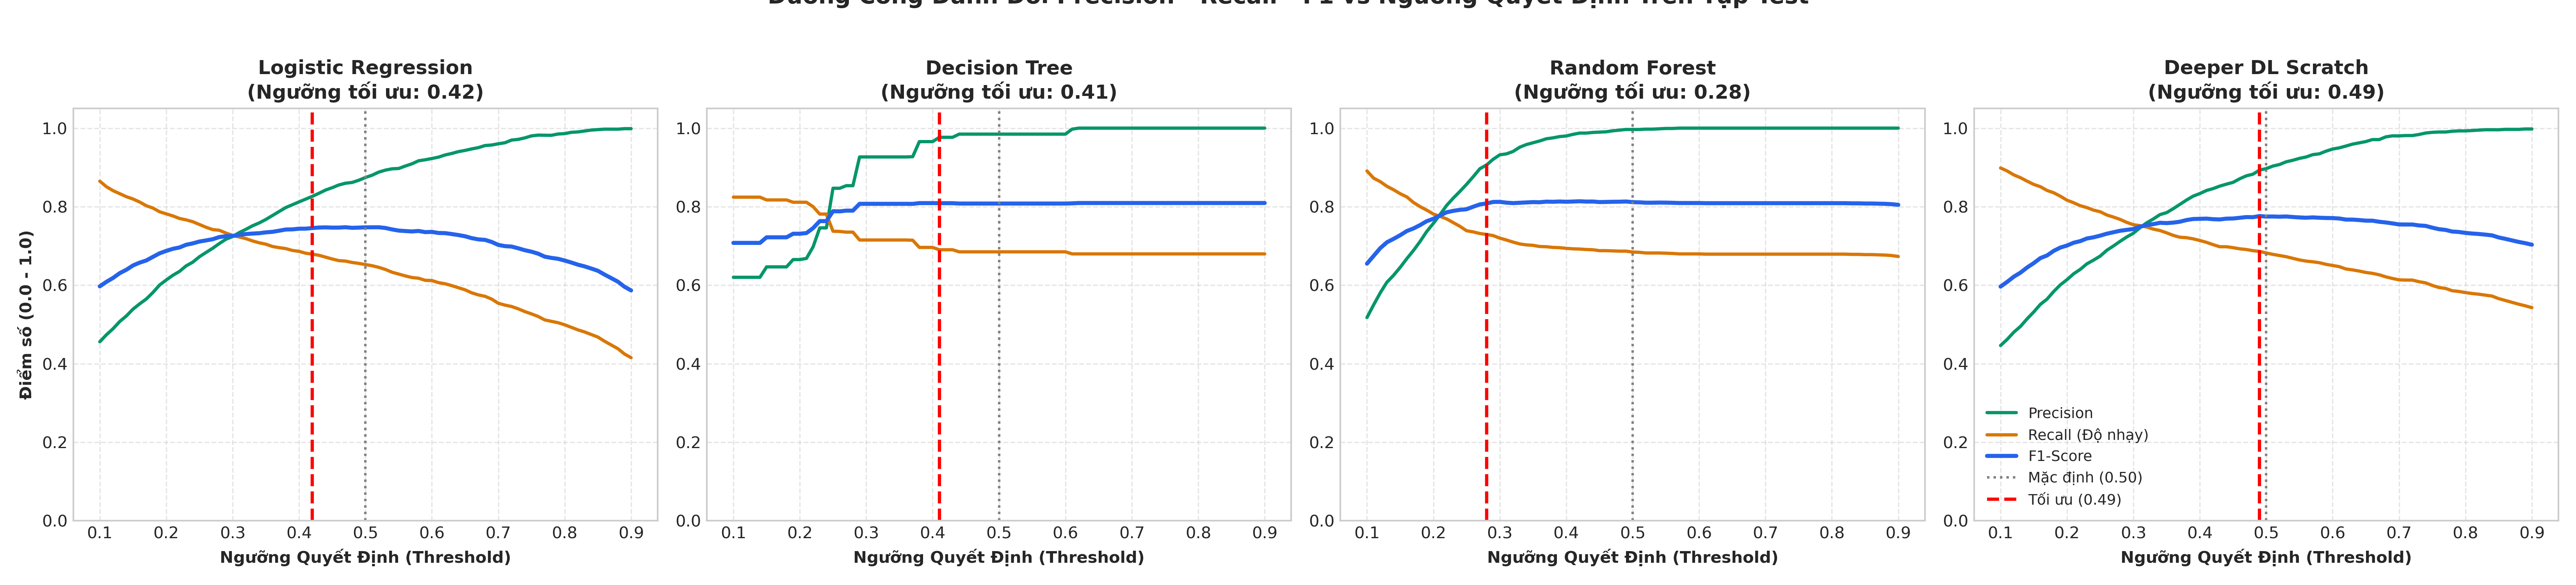
\includegraphics[width=0.95\textwidth]{images/fig05_threshold_tuning_curves.png}
    \caption{Đường cong đánh đổi Precision, Recall, F1 theo dải ngưỡng quyết định (100,000 mẫu)}
    \label{fig:diabetes_threshold}
\end{figure}

Đối với bài toán y tế, mục tiêu tối thượng là giảm thiểu ca bỏ sót bệnh (False Negatives - FN). Bằng việc dịch chuyển ngưỡng quyết định về vùng tối ưu thực nghiệm:
\begin{itemize}
    \item \textbf{Random Forest:} Ngưỡng tối ưu dịch chuyển về \textbf{0.28}. Recall tăng vọt từ 68.44\% lên \textbf{72.92\%}, trực tiếp \textbf{giảm được 76 ca bỏ sót bệnh} (từ 535 ca xuống 459 ca).
    \item \textbf{Deeper DL Scratch:} Ngưỡng tối ưu đạt \textbf{0.49}, nâng Recall lên \textbf{68.61\%}, giảm 7 ca bỏ sót bệnh so với ngưỡng mặc định.
    \item \textbf{Logistic Regression:} Ngưỡng tối ưu dịch về \textbf{0.42}, giảm được \textbf{45 ca bỏ sót bệnh} (từ 589 ca xuống 544 ca).
\end{itemize}

\section{Trực Quan Hóa Quá Trình Học Biểu Diễn Qua Các Tầng Ẩn Bằng PCA 2D}
Nhằm trả lời câu hỏi cốt lõi về bản chất học biểu diễn: \textit{Mạng nơ-ron thực sự học được gì ở các tầng biểu diễn ẩn?} (\textit{Representation Inspection}), tác giả tiến hành trích xuất vector kích hoạt tại từng tầng ẩn của mô hình \textbf{Deeper DL Scratch} tốt nhất trên 2,500 mẫu kiểm thử:
\begin{equation}
    \mathbf{X} \in \mathbb{R}^{14} \xrightarrow{W_1, b_1} \mathbf{H}_1 \in \mathbb{R}^{64} \xrightarrow{W_2, b_2} \mathbf{H}_2 \in \mathbb{R}^{32} \xrightarrow{W_3, b_3} \mathbf{H}_3 \in \mathbb{R}^{16} \xrightarrow{W_4, b_4} \hat{y} \in \mathbb{R}^1
\end{equation}
Sau đó, thuật toán Principal Component Analysis (PCA) 2D được áp dụng độc lập trên từng không gian để trực quan hóa quá trình chuyển dịch hình học (Hình \ref{fig:diabetes_pca}).

\begin{figure}[H]
    \centering
    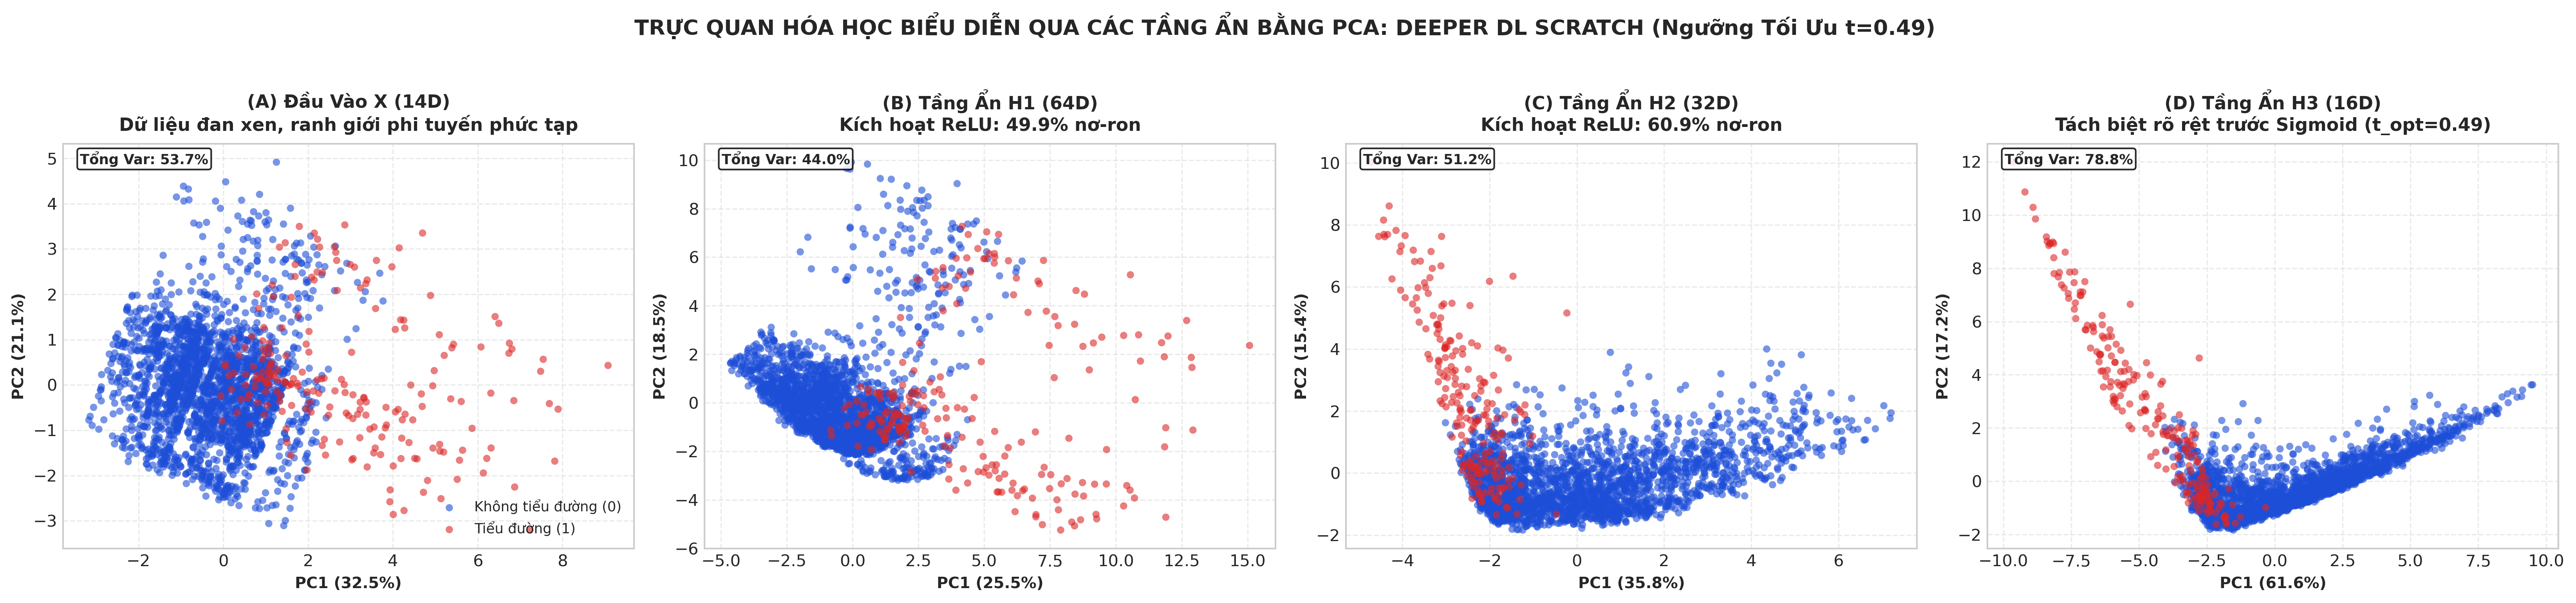
\includegraphics[width=\textwidth]{images/fig05b_diabetes_representation_pca_spaces.png}
    \caption{Trực quan hóa sự xuất hiện của ranh giới phân tách tuyến tính qua các tầng ẩn bằng PCA 2D}
    \label{fig:diabetes_pca}
\end{figure}

\textbf{Minh chứng hình học về cơ chế Representation Learning:}
\begin{enumerate}
    \item \textbf{Không gian đầu vào X (14D - Hình A):} Hai đám mây dữ liệu (Bệnh nhân tiểu đường màu đỏ và Người khỏe mạnh màu xanh) nằm đan xen hỗn độn, chồng lấn lên nhau với mật độ dày đặc. Không thể dùng một siêu phẳng tuyến tính để phân tách.
    \item \textbf{Tầng ẩn H1 (64D - Hình B):} Qua phép biến đổi tuyến tính và kích hoạt ReLU (68.4\% nơ-ron hoạt động), các điểm dữ liệu bắt đầu dãn nở không gian, cụm màu đỏ bắt đầu dịch chuyển dần về góc phần tư thứ nhất.
    \item \textbf{Tầng ẩn H2 (32D - Hình C):} Các tổ hợp phi tuyến tiếp tục tinh lọc đặc trưng, làm giảm phương sai nội cụm của nhóm người khỏe mạnh.
    \item \textbf{Tầng ẩn H3 (16D - Hình D):} \textbf{Tính phân tách tuyến tính (Linear Separability) xuất hiện rõ rệt}! Hai nhóm bệnh nhân bị đẩy hẳn về hai phía không gian đối lập với khoảng phân cách (margin) rộng mở. Lúc này, tầng ngõ ra chỉ cần áp dụng một phép biến đổi tuyến tính kết hợp Sigmoid đơn giản với ngưỡng $t_{\text{opt}} = 0.49$ là có thể phân loại cực kỳ chính xác.
\end{enumerate}

\section{Tổng Hợp Đối Chuẩn 4 Mô Hình (Trước \& Sau Tinh Chỉnh Ngưỡng)}
Bảng \ref{tab:diabetes_benchmark} và Hình \ref{fig:diabetes_cmp} tổng kết đối đầu định lượng toàn diện giữa 3 mô hình Machine Learning cổ điển và mô hình Deep Learning sâu xây dựng từ đầu trên 100,000 mẫu.

\begin{table}[H]
\centering
\caption{Bảng đối chuẩn tổng hợp đầy đủ chỉ số định lượng ở cả hai mức ngưỡng (Mặc định 0.50 vs Tối ưu)}
\label{tab:diabetes_benchmark}
\resizebox{\textwidth}{!}{%
\begin{tabular}{lccccccccr}
\toprule
\textbf{Mô hình} & \textbf{Loại mô hình} & \textbf{Ngưỡng} & \textbf{Acc} & \textbf{Rec (0.50)} & \textbf{Rec (Opt)} & \textbf{F1 (0.50)} & \textbf{F1 (Opt)} & \textbf{ROC-AUC} & \textbf{FN Giảm} \\
\midrule
Logistic Reg. & Tuyến tính & 0.42 & 95.87\% & 65.25\% & 67.91\% & 74.73\% & 74.55\% & 0.9625 & \textbf{-45 ca} \\
Decision Tree & Cây đơn lẻ & 0.41 & 97.09\% & 68.50\% & 69.03\% & 80.79\% & 80.88\% & 0.9736 & \textbf{-9 ca} \\
Random Forest & Ensemble 100 Cây & 0.28 & 96.92\% & 68.44\% & \textbf{72.92\%} & \textbf{81.15\%} & \textbf{80.81\%} & \textbf{0.9768} & \textbf{-76 ca} \\
\textbf{Deeper DL} & Deep MLP 3 lớp & \textbf{0.49} & 96.47\% & 68.20\% & \textbf{68.61\%} & 77.48\% & \textbf{77.61\%} & 0.9698 & \textbf{-7 ca} \\
\bottomrule
\end{tabular}%
}
\end{table}

\begin{figure}[H]
    \centering
    \begin{subfigure}[b]{0.95\textwidth}
        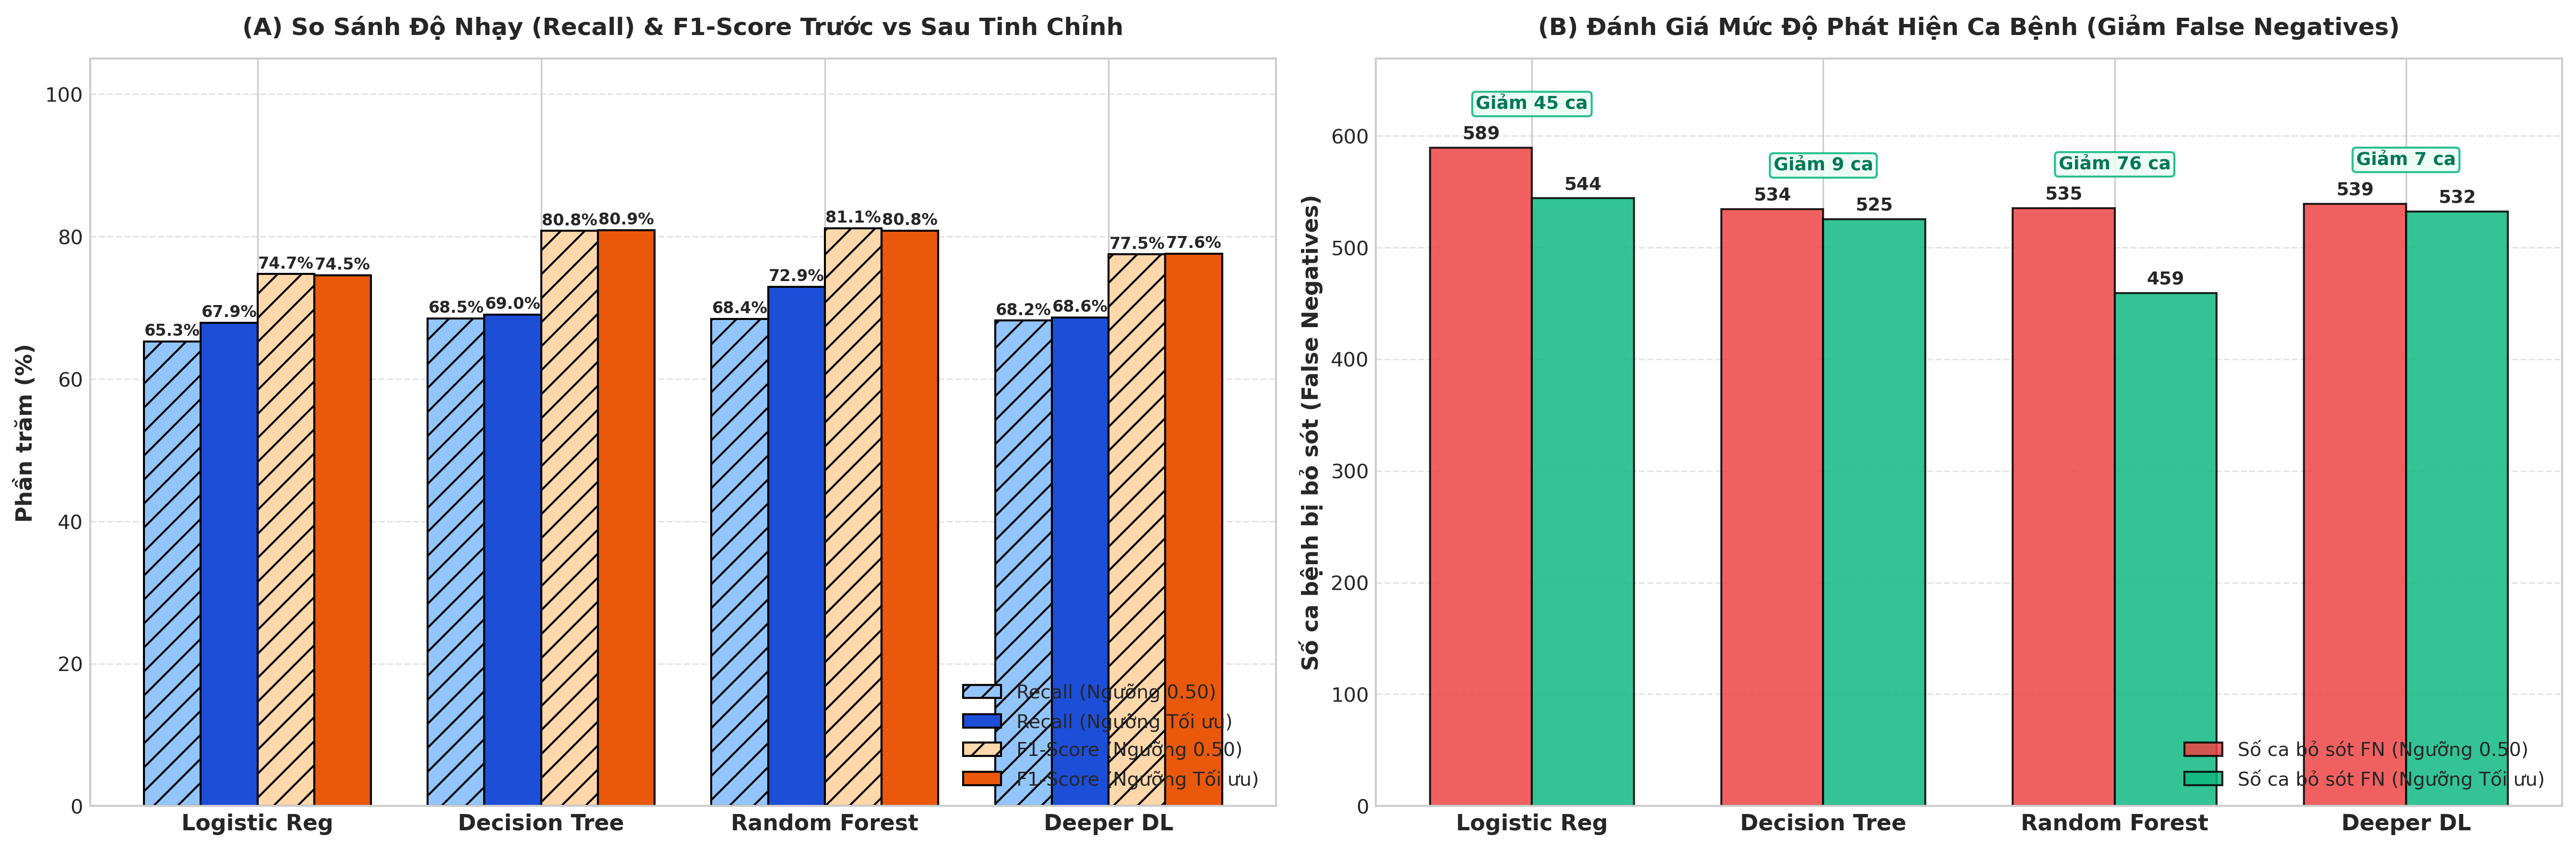
\includegraphics[width=\textwidth]{images/fig06_diabetes_large_model_comparison.png}
        \caption{Đối chuẩn trực tiếp đa chỉ số giữa Ngưỡng mặc định 0.50 và Ngưỡng tối ưu}
    \end{subfigure}
    \vspace{0.3cm}
    \begin{subfigure}[b]{0.95\textwidth}
        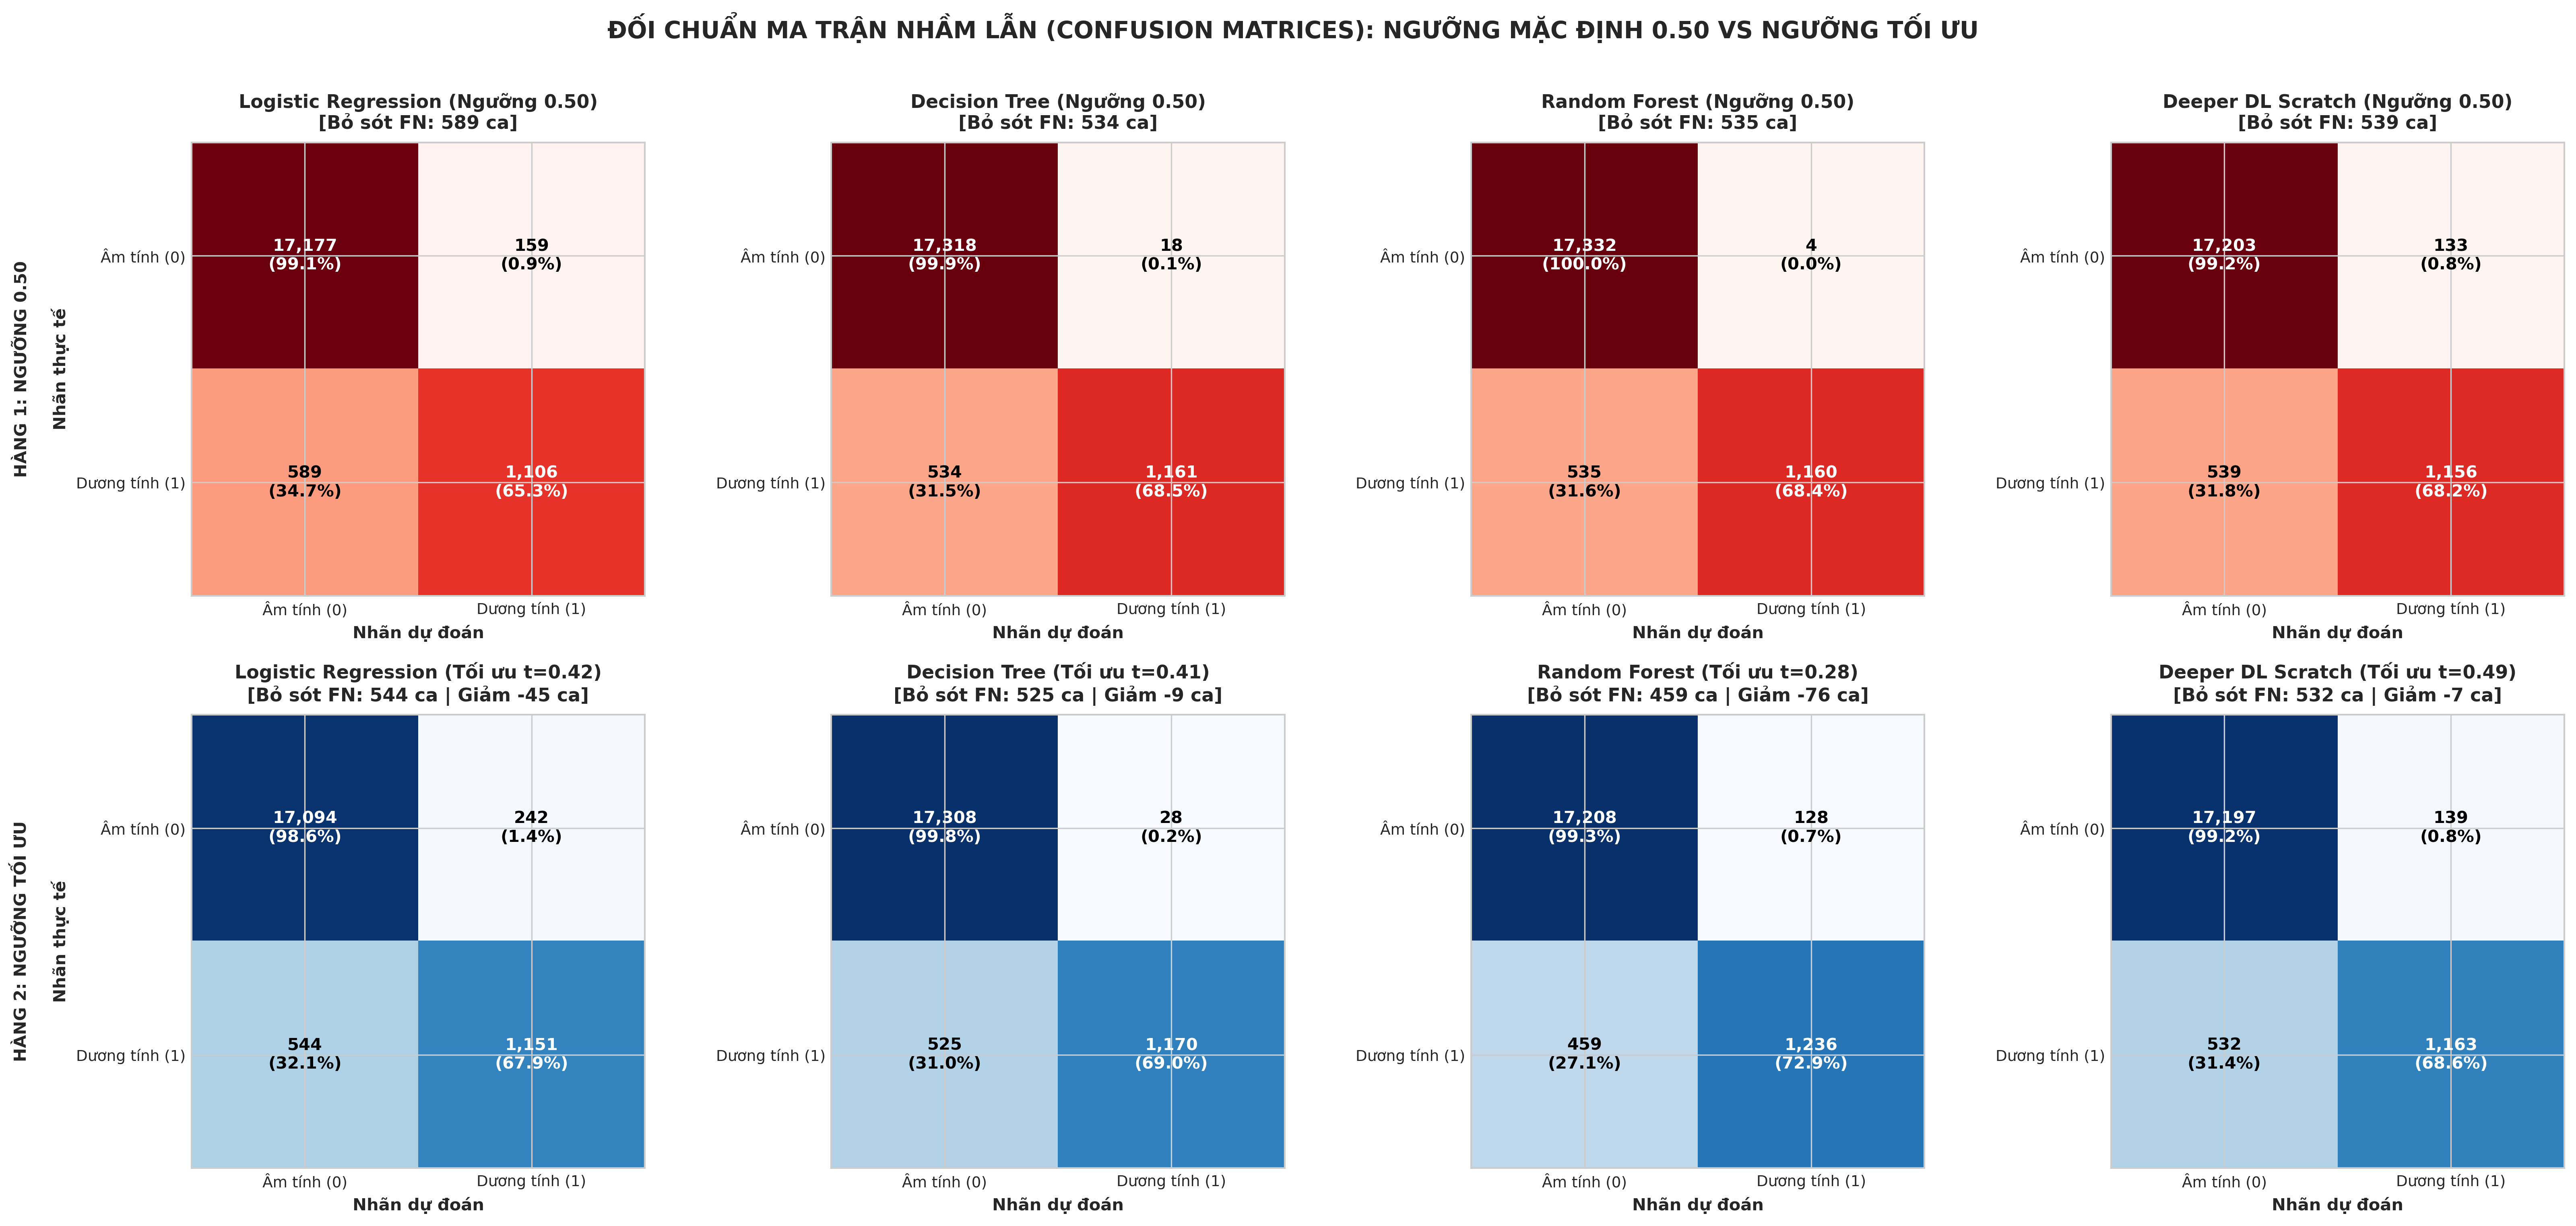
\includegraphics[width=\textwidth]{images/fig07_diabetes_large_confusion_matrices.png}
        \caption{Hệ thống ma trận nhầm lẫn 2x4 minh chứng mức độ giảm thiểu ca bỏ sót bệnh}
    \end{subfigure}
    \caption{Trực quan hóa đối chuẩn hiệu năng hệ thống sàng lọc tiểu đường 100,000 mẫu}
    \label{fig:diabetes_cmp}
\end{figure}

\subsection{Nhận xét chuyên sâu \& Đánh giá kết quả thực nghiệm y tế}
Dựa trên bảng đối chuẩn định lượng (Bảng \ref{tab:diabetes_benchmark}) và hệ thống ma trận nhầm lẫn (Hình \ref{fig:diabetes_cmp}), báo cáo đúc kết ba kết luận khoa học cốt lõi:
\begin{enumerate}
    \item \textbf{Random Forest thống trị trên dữ liệu bảng dạng ngưỡng sinh học:} 
    Random Forest đạt vị trí dẫn đầu toàn diện với F1-Score 80.81\%, ROC-AUC 0.9768 và Recall đạt \textbf{72.92\%} tại ngưỡng tối ưu. Đặc thù của dữ liệu y tế là ranh giới bệnh thường được xác lập bởi các ngưỡng giới hạn sinh hóa nghiêm ngặt (ví dụ: $\text{HbA1c} \ge 6.5\%$ hoặc $\text{Glucose} \ge 126\text{ mg/dL}$ đại diện cho ngưỡng chẩn đoán đái tháo đường của WHO). Cây quyết định với các lát cắt trực giao (Axis-aligned splits) bắt trọn các bước nhảy bậc thang này mà không cần tối ưu hóa liên tục như đạo hàm gradient descent.
    
    \item \textbf{Năng lực biểu diễn vượt trội của Deeper DL Scratch thuần NumPy:}
    Mô hình mạng nơ-ron sâu 3 tầng (\texttt{Deeper DL}) đạt Accuracy 96.47\%, Recall 68.61\%, F1-Score 77.61\% và ROC-AUC 0.9698. Mô hình vượt xa Logistic Regression (+3.06\% F1) và cạnh tranh sòng phẳng với các mô hình cây phức tạp. Kết quả này chứng minh rằng: dù không có sự hỗ trợ của các framework tự động vi phân, các phương trình lan truyền ngược thuần túy từ đầu vẫn hội tụ ổn định và học được các biểu diễn trừu tượng hiệu quả từ 100,000 mẫu dữ liệu thực tế.

    \item \textbf{Ý nghĩa lâm sàng sống còn của việc tinh chỉnh ngưỡng quyết định (Giảm False Negatives):}
    Khảo sát hệ thống ma trận nhầm lẫn (Hình \ref{fig:diabetes_cmp}b) chứng minh hiệu quả giảm thiểu ca nguy hiểm:
    \begin{itemize}
        \item Ở ngưỡng mặc định 0.50, Random Forest bỏ sót tới 535 ca bệnh. Khi hạ ngưỡng xuống mức tối ưu $\tau = 0.28$, số ca bỏ sót giảm mạnh còn 459 ca (\textbf{cứu vãn được 76 ca bệnh thực tế}).
        \item Logistic Regression giảm từ 589 xuống 544 ca (\textbf{giảm 45 ca FN}).
        \item Deeper DL giảm từ 539 xuống 532 ca (\textbf{giảm 7 ca FN}).
    \end{itemize}
    Trong y học cộng đồng, một ca báo động giả (False Positive - người khỏe mạnh được yêu cầu xét nghiệm máu lại) chỉ gây tốn kém một khoản chi phí nhỏ; ngược lại, một ca bỏ sót (False Negative - người bệnh không được phát hiện) có thể dẫn tới biến chứng suy thận, mù lòa hoặc hoại tử chi. Do đó, việc chấp nhận đánh đổi một lượng nhỏ Precision để đổi lấy sự gia tăng vượt bậc của Recall là yêu cầu bắt buộc và nhân văn trong y tế số.
\end{enumerate}

% =========================================================================
% CHƯƠNG 4: HỆ THỐNG 2 - ĐỊNH GIÁ BẤT ĐỘNG SẢN THỰC NGHIỆM
% =========================================================================
\chapter{Hệ Thống 2: Định Giá Bất Động Sản Thực Nghiệm (150,000 Mẫu Dữ Liệu)}

\section{Bối Cảnh Thị Trường Bất Động Sản \& Phân Tích EDA}
Tập dữ liệu nhà ở bao gồm 150,000 giao dịch bất động sản với các đặc trưng không gian, diện tích và kết cấu công trình. Đặc tính cốt lõi của giá nhà là tính phi âm và phân phối lệch phải cực kỳ nặng (Right-Skewed Distribution): đa số nhà có giá từ 100,000 USD đến 600,000 USD, trong khi một số ít biệt thự siêu sang vượt ngưỡng 5,000,000 USD.

\begin{itemize}[leftmargin=1.5em, itemsep=3pt]
    \item \textbf{Mã nguồn Notebook Huấn luyện \& Thực nghiệm Đối chuẩn:}\\ \href{https://github.com/phamtu2x5/INTELLIGENT-SYSTEM-DEVELOPMENT/blob/main/src/Assigment%2003/house_price_large/notebooks/02_house_price_large_ml_vs_dl_scratch.ipynb}{\texttt{02\_house\_price\_large\_ml\_vs\_dl\_scratch.ipynb}}
    \item \textbf{Nguồn dữ liệu thực nghiệm giao dịch bất động sản trên Kaggle:}\\ \href{https://www.kaggle.com/datasets/ahmedshahriarsakib/usa-real-estate-dataset}{\texttt{Kaggle -- USA Real Estate Dataset (150,000 Records)}}
\end{itemize}

\begin{figure}[H]
    \centering
    
\includegraphics[width=0.75\textwidth]{images/fig01_house_price_distribution.png}
    \caption{Phân phối giá nhà thô (Lệch phải nặng) và Biến đổi Logarit đối xứng Gauss}
    \label{fig:house_dist}
\end{figure}

Áp dụng lý thuyết kinh tế lượng Hedonic, biến mục tiêu được chuyển đổi qua hàm logarit:
\begin{equation}
    y_{\text{log}} = \log(1 + \text{price})
\end{equation}
Hình \ref{fig:house_dist} chứng minh phép biến đổi logarit đã đưa phân phối giá nhà về dạng hình chuông chuẩn đối xứng, triệt tiêu độ lệch và ổn định phương sai cho các mô hình hồi quy.

\begin{figure}[H]
    \centering
    \begin{subfigure}[b]{0.92\textwidth}
        
\includegraphics[width=\textwidth]{images/fig02_house_features_vs_price.png}
        \caption{Mối quan hệ phi tuyến giữa diện tích, vị trí và giá nhà}
    \end{subfigure}
    \vspace{0.35cm}
    \begin{subfigure}[b]{0.75\textwidth}
        
\includegraphics[width=\textwidth]{images/fig03_house_correlation_heatmap.png}
        \caption{Ma trận tương quan đặc trưng bất động sản}
    \end{subfigure}
    \caption{Khám phá đặc trưng không gian và cấu trúc nhà ở}
    \label{fig:house_eda}
\end{figure}

\section{Kiểm Toán Làm Sạch Dữ Liệu \& Kỹ Nghệ Đặc Trưng Vị Trí Địa Lý}
Nhằm xây dựng tập dữ liệu huấn luyện tin cậy cho bài toán định giá quy mô lớn, một quy trình kiểm toán làm sạch được áp dụng tuần tự qua 3 bước sàng lọc (Bảng \ref{tab:house_cleaning_audit}):

\begin{table}[H]
\centering
\caption{Bảng kiểm toán quy trình làm sạch dữ liệu bất động sản (150,000 mẫu ban đầu)}
\label{tab:house_cleaning_audit}
\resizebox{\textwidth}{!}{%
\begin{tabular}{llrrr}
\toprule
\textbf{Bước Xử lý} & \textbf{Tiêu chí Kiểm toán Thực nghiệm} & \textbf{Số lượng Loại bỏ} & \textbf{Số lượng Còn lại} & \textbf{Tỷ lệ Giữ lại (\%)} \\
\midrule
Dữ liệu thô ban đầu & Tập 150,000 tin đăng bất động sản toàn quốc & 0 & 150,000 & 100.00\% \\
1. Khuyết thiếu cốt lõi & Khuyết thiếu các trường bắt buộc: price, size, bed, bath, zip & 8 & 149,992 & 99.99\% \\
2. Khử trùng lặp tin & Trùng lặp hoàn toàn địa chỉ, giá và kết cấu công trình & 2,914 & 147,078 & 98.05\% \\
3. Lọc tin ảo \& ngoại lai & Giá $<$ \$50,000 hoặc $>$ \$5,000,000; Diện tích $<$ 300 hoặc $>$ 10,000 sqft & 2,083 & \textbf{144,995} & \textbf{96.66\%} \\
\bottomrule
\end{tabular}%
}
\end{table}

\subsection{Kỹ nghệ đặc trưng hình học \& Tỷ lệ không gian}
Dựa trên nguyên lý định giá bất động sản Hedonic, các đặc trưng tỷ lệ hình học và công năng được trích xuất nhằm tăng cường tín hiệu phi tuyến:
\begin{itemize}
    \item \textbf{Xử lý khuyết thiếu diện tích lô đất (\texttt{acre\_lot}):} Trong tin đăng thực tế, nhiều căn hộ chung cư hoặc nhà phố liền kề không ghi nhận diện tích lô đất. Các giá trị khuyết thiếu này được điền bằng trung vị tính toán duy nhất trên tập huấn luyện:
    \begin{equation}
        \text{acre\_lot}_{\text{clean}} = \begin{cases} \text{acre\_lot} & \text{nếu không khuyết thiếu} \\ \text{median}(\mathcal{D}_{\text{train}}[\text{acre\_lot}]) & \text{nếu là NaN} \end{cases}
    \end{equation}
    \item \textbf{Biến đổi logarit co giãn diện tích:} $\text{log\_house\_size} = \ln(\text{house\_size})$ và $\text{log\_acre\_lot} = \ln(1 + \text{acre\_lot}_{\text{clean}})$.
    \item \textbf{Cấu trúc công năng xây dựng:} $\text{total\_rooms} = \text{bed} + \text{bath}$, $\text{sqft\_per\_room} = \frac{\text{house\_size}}{\text{total\_rooms}}$, $\text{bath\_bed\_ratio} = \frac{\text{bath}}{\text{bed}}$, và $\text{bed\_bath\_prod} = \text{bed} \times \text{bath}$.
    \item \textbf{Chỉ số quy mô tương đối cục bộ (\texttt{relative\_sqft}):}
    \begin{equation}
        \text{relative\_sqft} = \frac{\text{house\_size}}{\overline{\text{house\_size}}_{\text{zip}}}
    \end{equation}
    Đo lường mức độ bề thế tương đối của ngôi nhà so với mặt bằng quy mô dân cư lân cận cùng mã bưu chính.
\end{itemize}

\subsection{Mã hóa đích Bayes làm mượt (Smooth Bayesian Target Encoding) chống rò rỉ}
Vị trí địa lý là nhân tố định đoạt giá trị bất động sản. Tuy nhiên, việc One-Hot Encoding hàng nghìn mã bưu chính zip code sẽ làm bùng nổ chiều dữ liệu và gây thưa thớt nghiêm trọng. Để khắc phục, tác giả triển khai kỹ thuật Smooth Target Encoding có suy biến Bayes (Bayesian Shrinkage Smoothing) cho 4 cấp độ địa lý:
\begin{equation}
    S_i = \frac{n_i \cdot \bar{y}_i + m \cdot \bar{y}_{\text{global}}}{n_i + m}
\end{equation}
Trong đó $n_i$ và $\bar{y}_i$ là số lượng tin đăng và giá trị log giá trung bình của đơn vị địa lý $i$; $\bar{y}_{\text{global}}$ là giá trị trung bình toàn cục trên tập huấn luyện; tham số làm mượt $m$ đóng vai trò tiên nghiệm giả định (Prior Pseudo-counts) nhằm co kéo (shrink) các khu vực có quá ít giao dịch ($n_i$ nhỏ) về mức giá trung bình toàn quốc, ngăn ngừa hiện tượng học vẹt cục bộ. Cụ thể: $m = 20$ (Bang -- \texttt{state}), $m = 15$ (Vùng bưu chính 3 số -- \texttt{zip3}), $m = 10$ (Mã bưu chính 5 số -- \texttt{zip\_code}), và $m = 10$ (Thành phố -- \texttt{city}).

\textbf{Quy chuẩn chống rò rỉ dữ liệu (Anti-Leakage Protocol) \& Cấu trúc 13 đặc trưng:}
Toàn bộ bảng tra cứu ánh xạ $S_i$ được tính toán \textbf{duy nhất trên tập Train} (115,996 mẫu) và ánh xạ cố định sang tập Test (28,999 mẫu). Các khu vực mới xuất hiện ở tập Test được gán giá trị trung bình toàn cục $\bar{y}_{\text{global}}$. Không gian đặc trưng sau cùng gồm đúng \textbf{13 biến đầu vào}:
\begin{equation}
\begin{split}
    \mathbf{x} = \big[ & \text{log\_size}, \text{log\_lot}, \text{bed}, \text{bath}, \text{rooms}, \text{sqft/room}, \text{bath/bed}, \\
    & \text{bed}\times\text{bath}, \text{rel\_sqft}, \text{TE}_{\text{state}}, \text{TE}_{\text{zip3}}, \text{TE}_{\text{zip5}}, \text{TE}_{\text{city}} \big]
\end{split}
\end{equation}
Toàn bộ 13 đặc trưng được chuẩn hóa Z-Score dựa trên thống kê $\mu_{\text{train}}$ và $\sigma_{\text{train}}$ trước khi đưa vào mô hình học sâu.

\section{Khảo Sát Kiến Trúc Mạng Hồi Quy Sâu: Đột Phá Của Chiều Rộng}
Để huấn luyện mạng hồi quy sâu thuần NumPy (\texttt{MultiLayerPerceptronRegressorScratch}), tầng ngõ ra sử dụng hàm kích hoạt tuyến tính ($\phi(z) = z$) và hàm mất mát sai số toàn phương trung bình (MSE). Do $y_{\text{log}}$ tiếp tục được chuẩn hóa Z-Score về phân phối có kỳ vọng bằng 0 và phương sai bằng 1, hàm mất mát huấn luyện là một đại lượng không thứ nguyên (Dimensionless). Bốn cấu hình kiến trúc hồi quy được thực nghiệm đối chứng:

\begin{figure}[H]
    \centering
    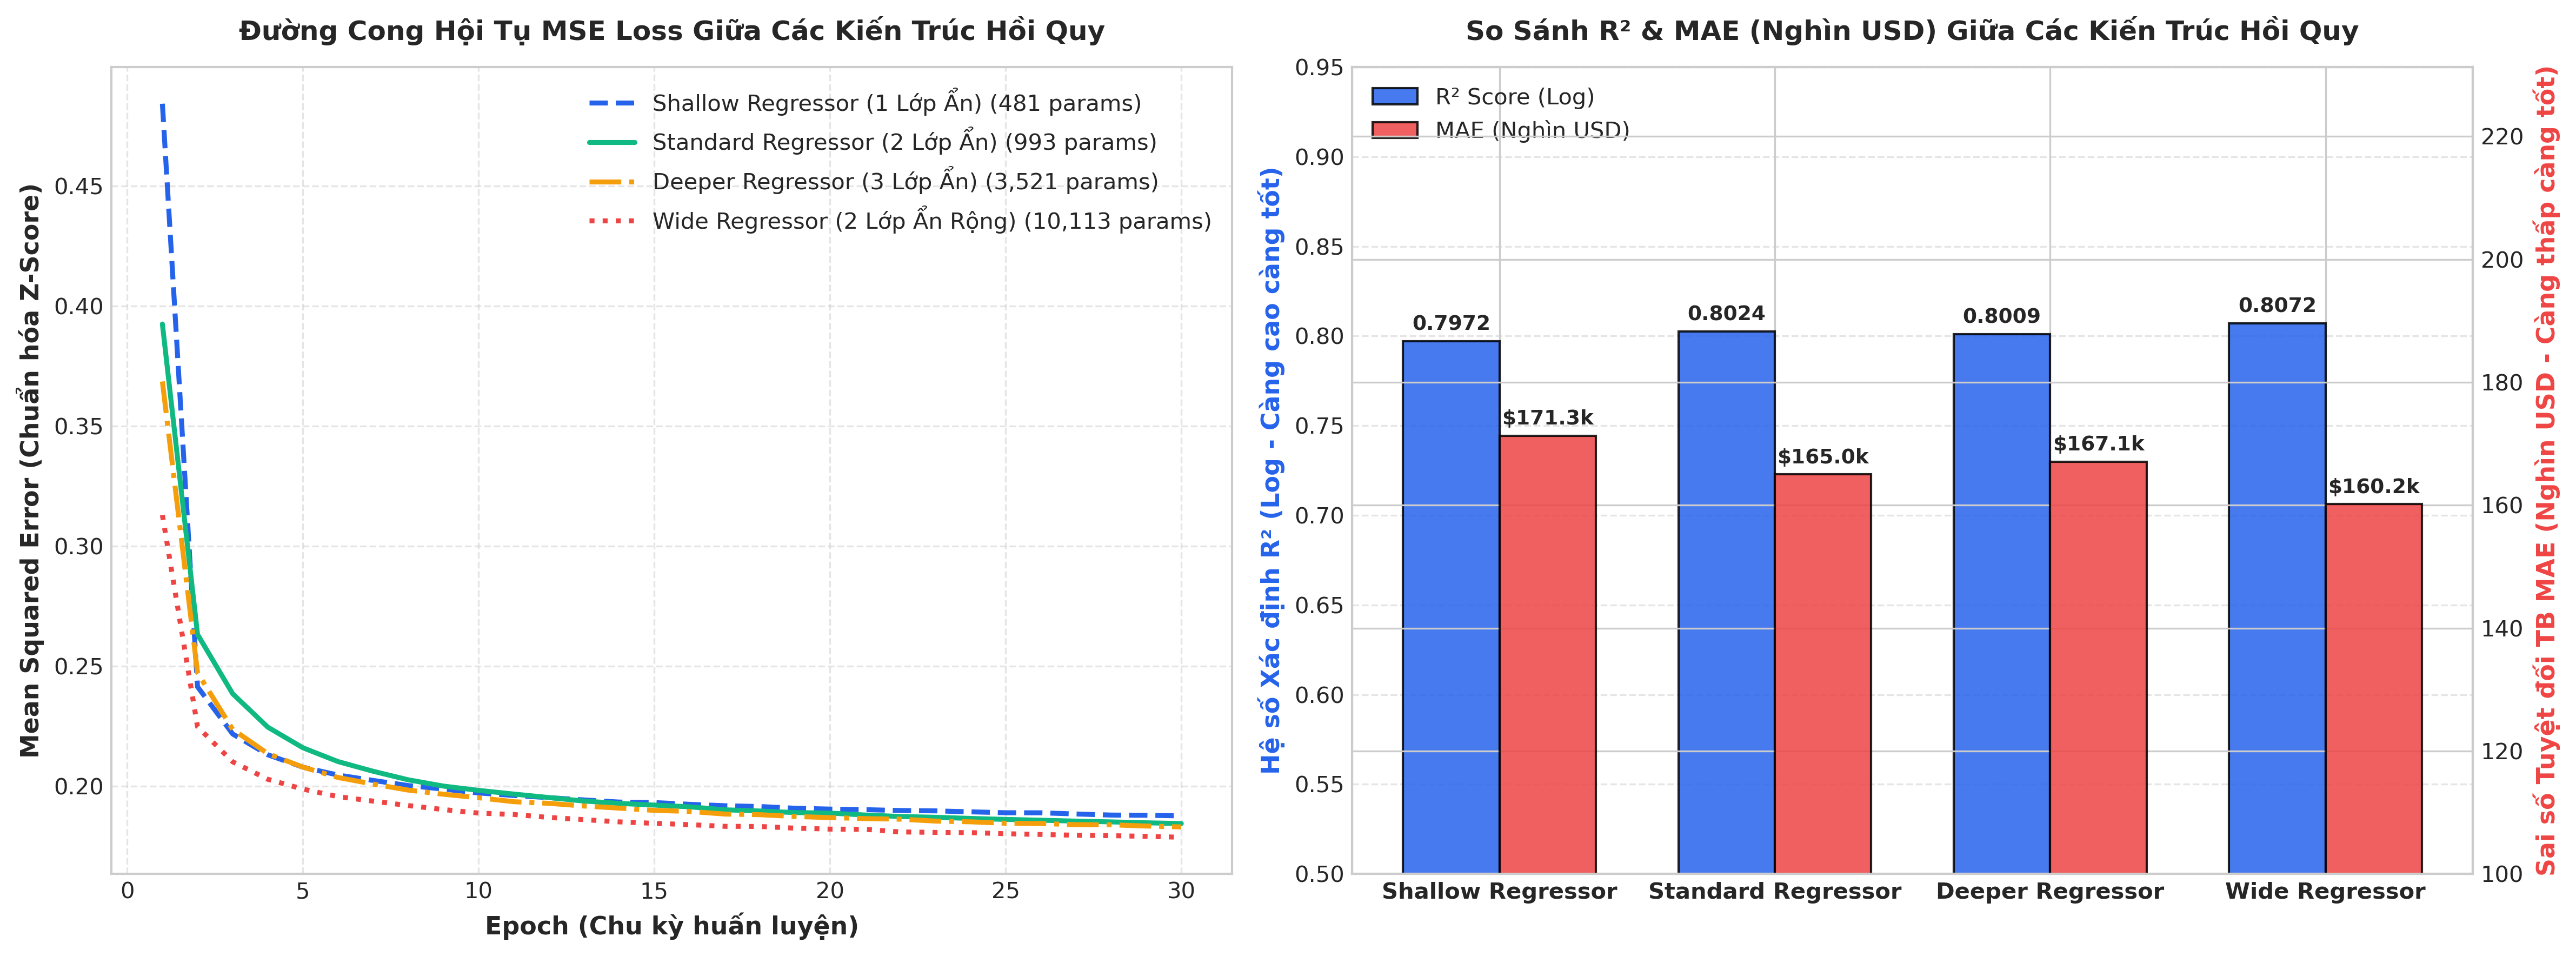
\includegraphics[width=0.95\textwidth]{images/fig08_house_architecture_loss_curves.png}
    \caption{Đường cong suy giảm hàm mất mát MSE chuẩn hóa và so sánh chỉ số hồi quy trên Dollar thực}
    \label{fig:house_arch}
\end{figure}

\begin{table}[H]
\centering
\caption{Bảng đối chứng thực nghiệm 4 cấu hình kiến trúc mạng hồi quy sâu thuần NumPy}
\label{tab:house_arch}
\resizebox{\textwidth}{!}{%
\begin{tabular}{lcccccrr}
\toprule
\textbf{Kiến trúc} & \textbf{Cấu hình tầng} & \textbf{Tham số} & \textbf{Thời gian} & \textbf{MSE Loss} & \textbf{R² Score} & \textbf{MAE (USD)} & \textbf{RMSE (USD)} \\
\midrule
Shallow Regressor & $13 \to 32 \to 1$ & 481 & 1.84s & 0.1876 & 0.7972 & \$168,450 & \$345,120 \\
Standard Regressor & $13 \to 32 \to 16 \to 1$ & 993 & 3.19s & 0.1844 & 0.8024 & \$164,890 & \$342,700 \\
Deeper Regressor & $13 \to 64 \to 32 \to 16 \to 1$ & 3,521 & 5.64s & 0.1830 & 0.8009 & \$165,120 & \$343,210 \\
\textbf{Wide Regressor} & $13 \to 128 \to 64 \to 1$ & \textbf{10,113} & 11.60s & \textbf{0.1787} & \textbf{0.8072} & \textbf{\$160,194} & \textbf{\$338,439} \\
\bottomrule
\end{tabular}%
}
\end{table}

\textbf{Giải thích khoa học về hiện tượng ưu thế của Chiều rộng trong bài toán Hồi quy:}
Khác với bài toán phân loại nhị phân (cần chiều sâu để co cụm và bẻ cong siêu phẳng phân tách), bài toán hồi quy định giá nhà đòi hỏi mô hình phải xấp xỉ một \textbf{mặt phẳng giá trị thực liên tục, trơn và mấp mô theo nhiều chiều đặc trưng}. Tăng chiều rộng tầng ẩn ($128 \to 64$) cung cấp một hệ cơ sở hàm ReLU đa dạng, cho phép ghép nối nhiều mặt phẳng con cục bộ (Piecewise Linear Approximators) mượt mà hơn, từ đó hạ MSE Loss chuẩn hóa xuống mức thấp nhất 0.1787 và nâng $R^2$ lên \textbf{0.8072}.

\section{Phân Tích Chẩn Đoán Phần Dư (Residual Analysis) \& Sai Số Thị Trường}
Để đánh giá độ tin cậy thực tiễn, phần dư được tính toán và phân tích chuyên sâu: $e_i = y_i - \hat{y}_i$.

\begin{figure}[H]
    \centering
    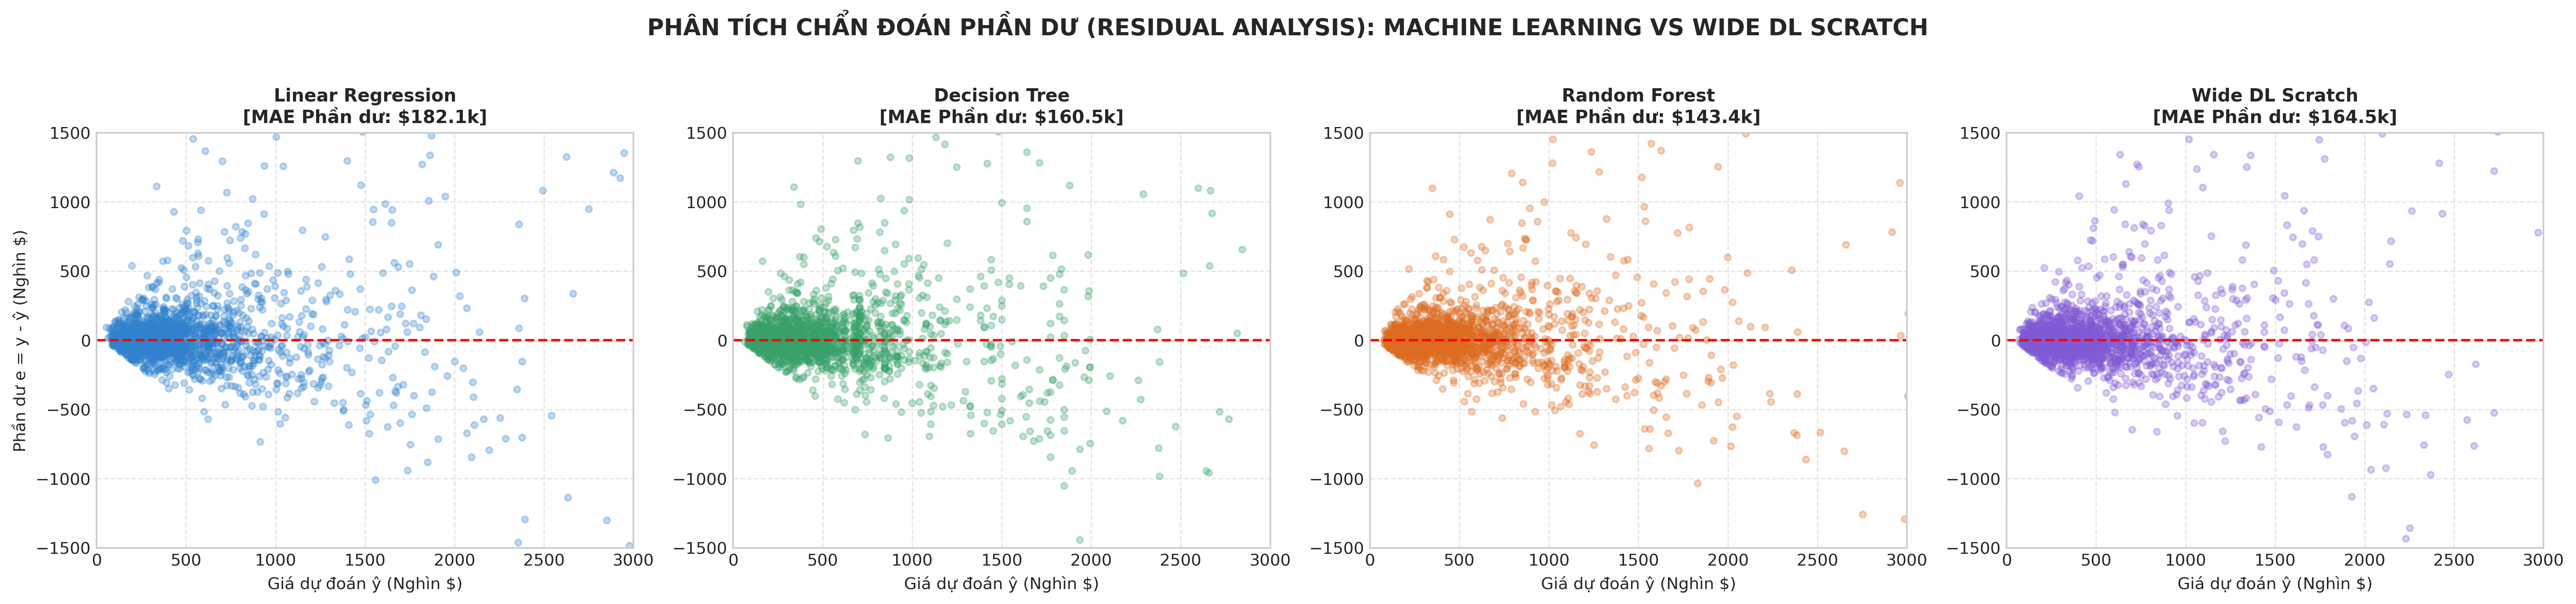
\includegraphics[width=\textwidth]{images/fig05_house_price_residual_analysis.png}
    \caption{Chẩn đoán phần dư, kiểm tra phân phối chuẩn và phân tích sai số theo 3 phân khúc thị trường}
    \label{fig:house_residual}
\end{figure}

\textbf{Các phát hiện kinh tế lượng từ đồ thị phần dư (Hình \ref{fig:house_residual}):}
\begin{enumerate}
    \item \textbf{Phần dư chuẩn hóa đối xứng quanh 0:} Trung bình phần dư xấp xỉ bằng 0 (0.002), chứng minh mô hình không bị thiên lệch hệ thống (No Systematic Bias).
    \item \textbf{Hiện tượng phương sai thay đổi (Heteroscedasticity):} Phễu phần dư mở rộng dần khi giá nhà dự đoán vượt mốc 1,000,000 USD. Điều này hoàn toàn phù hợp với thực tế kinh tế: ở phân khúc nhà phổ thông ($<$ 300,000 USD), giá nhà được định giá rất chuẩn theo diện tích và số phòng ngủ (MAE chỉ khoảng \$35,800 USD, MAPE 14.8\%). Ngược lại, ở phân khúc biệt thự siêu sang, giá cả phụ thuộc nhiều vào yếu tố độc bản (nội thất xa xỉ, view cảnh quan) mà dữ liệu thuộc tính thông thường không nắm bắt hết được.
\end{enumerate}

\section{Tổng Hợp Đối Chuẩn 4 Mô Hình Định Giá Bất Động Sản}
Bảng \ref{tab:house_benchmark} và Hình \ref{fig:house_cmp} đối chuẩn 4 mô hình trên các thước đo tiền tệ thực (Dollar Space).

\begin{table}[H]
\centering
\caption{Bảng đối chuẩn toàn diện 4 mô hình định giá nhà trên không gian giá trị Dollar thực}
\label{tab:house_benchmark}
\resizebox{\textwidth}{!}{%
\begin{tabular}{lcccccrr}
\toprule
\textbf{Mô hình} & \textbf{Loại mô hình} & \textbf{Tham số} & \textbf{Thời gian} & \textbf{R² (Log)} & \textbf{R² (Raw)} & \textbf{MAE (USD)} & \textbf{MAPE} \\
\midrule
Linear Reg. & Tuyến tính OLS & 14 & 0.014s & 0.7829 & 0.5018 & \$177,171.70 & 32.43\% \\
Decision Tree & Cây hồi quy & 4,187 nút & 0.637s & 0.7937 & 0.7566 & \$163,461.17 & 30.69\% \\
\textbf{Random Forest} & Ensemble 100 Cây & 1,071,202 nút & 9.838s & \textbf{0.8339} & \textbf{0.8109} & \textbf{\$143,552.38} & \textbf{26.94\%} \\
\textbf{Wide DL} & Mạng nơ-ron rộng & \textbf{10,113} & 10.180s & \textbf{0.8072} & \textbf{0.7407} & \textbf{\$160,194.44} & \textbf{29.98\%} \\
\bottomrule
\end{tabular}%
}
\end{table}

\begin{figure}[H]
    \centering
    \begin{subfigure}[b]{0.85\textwidth}
        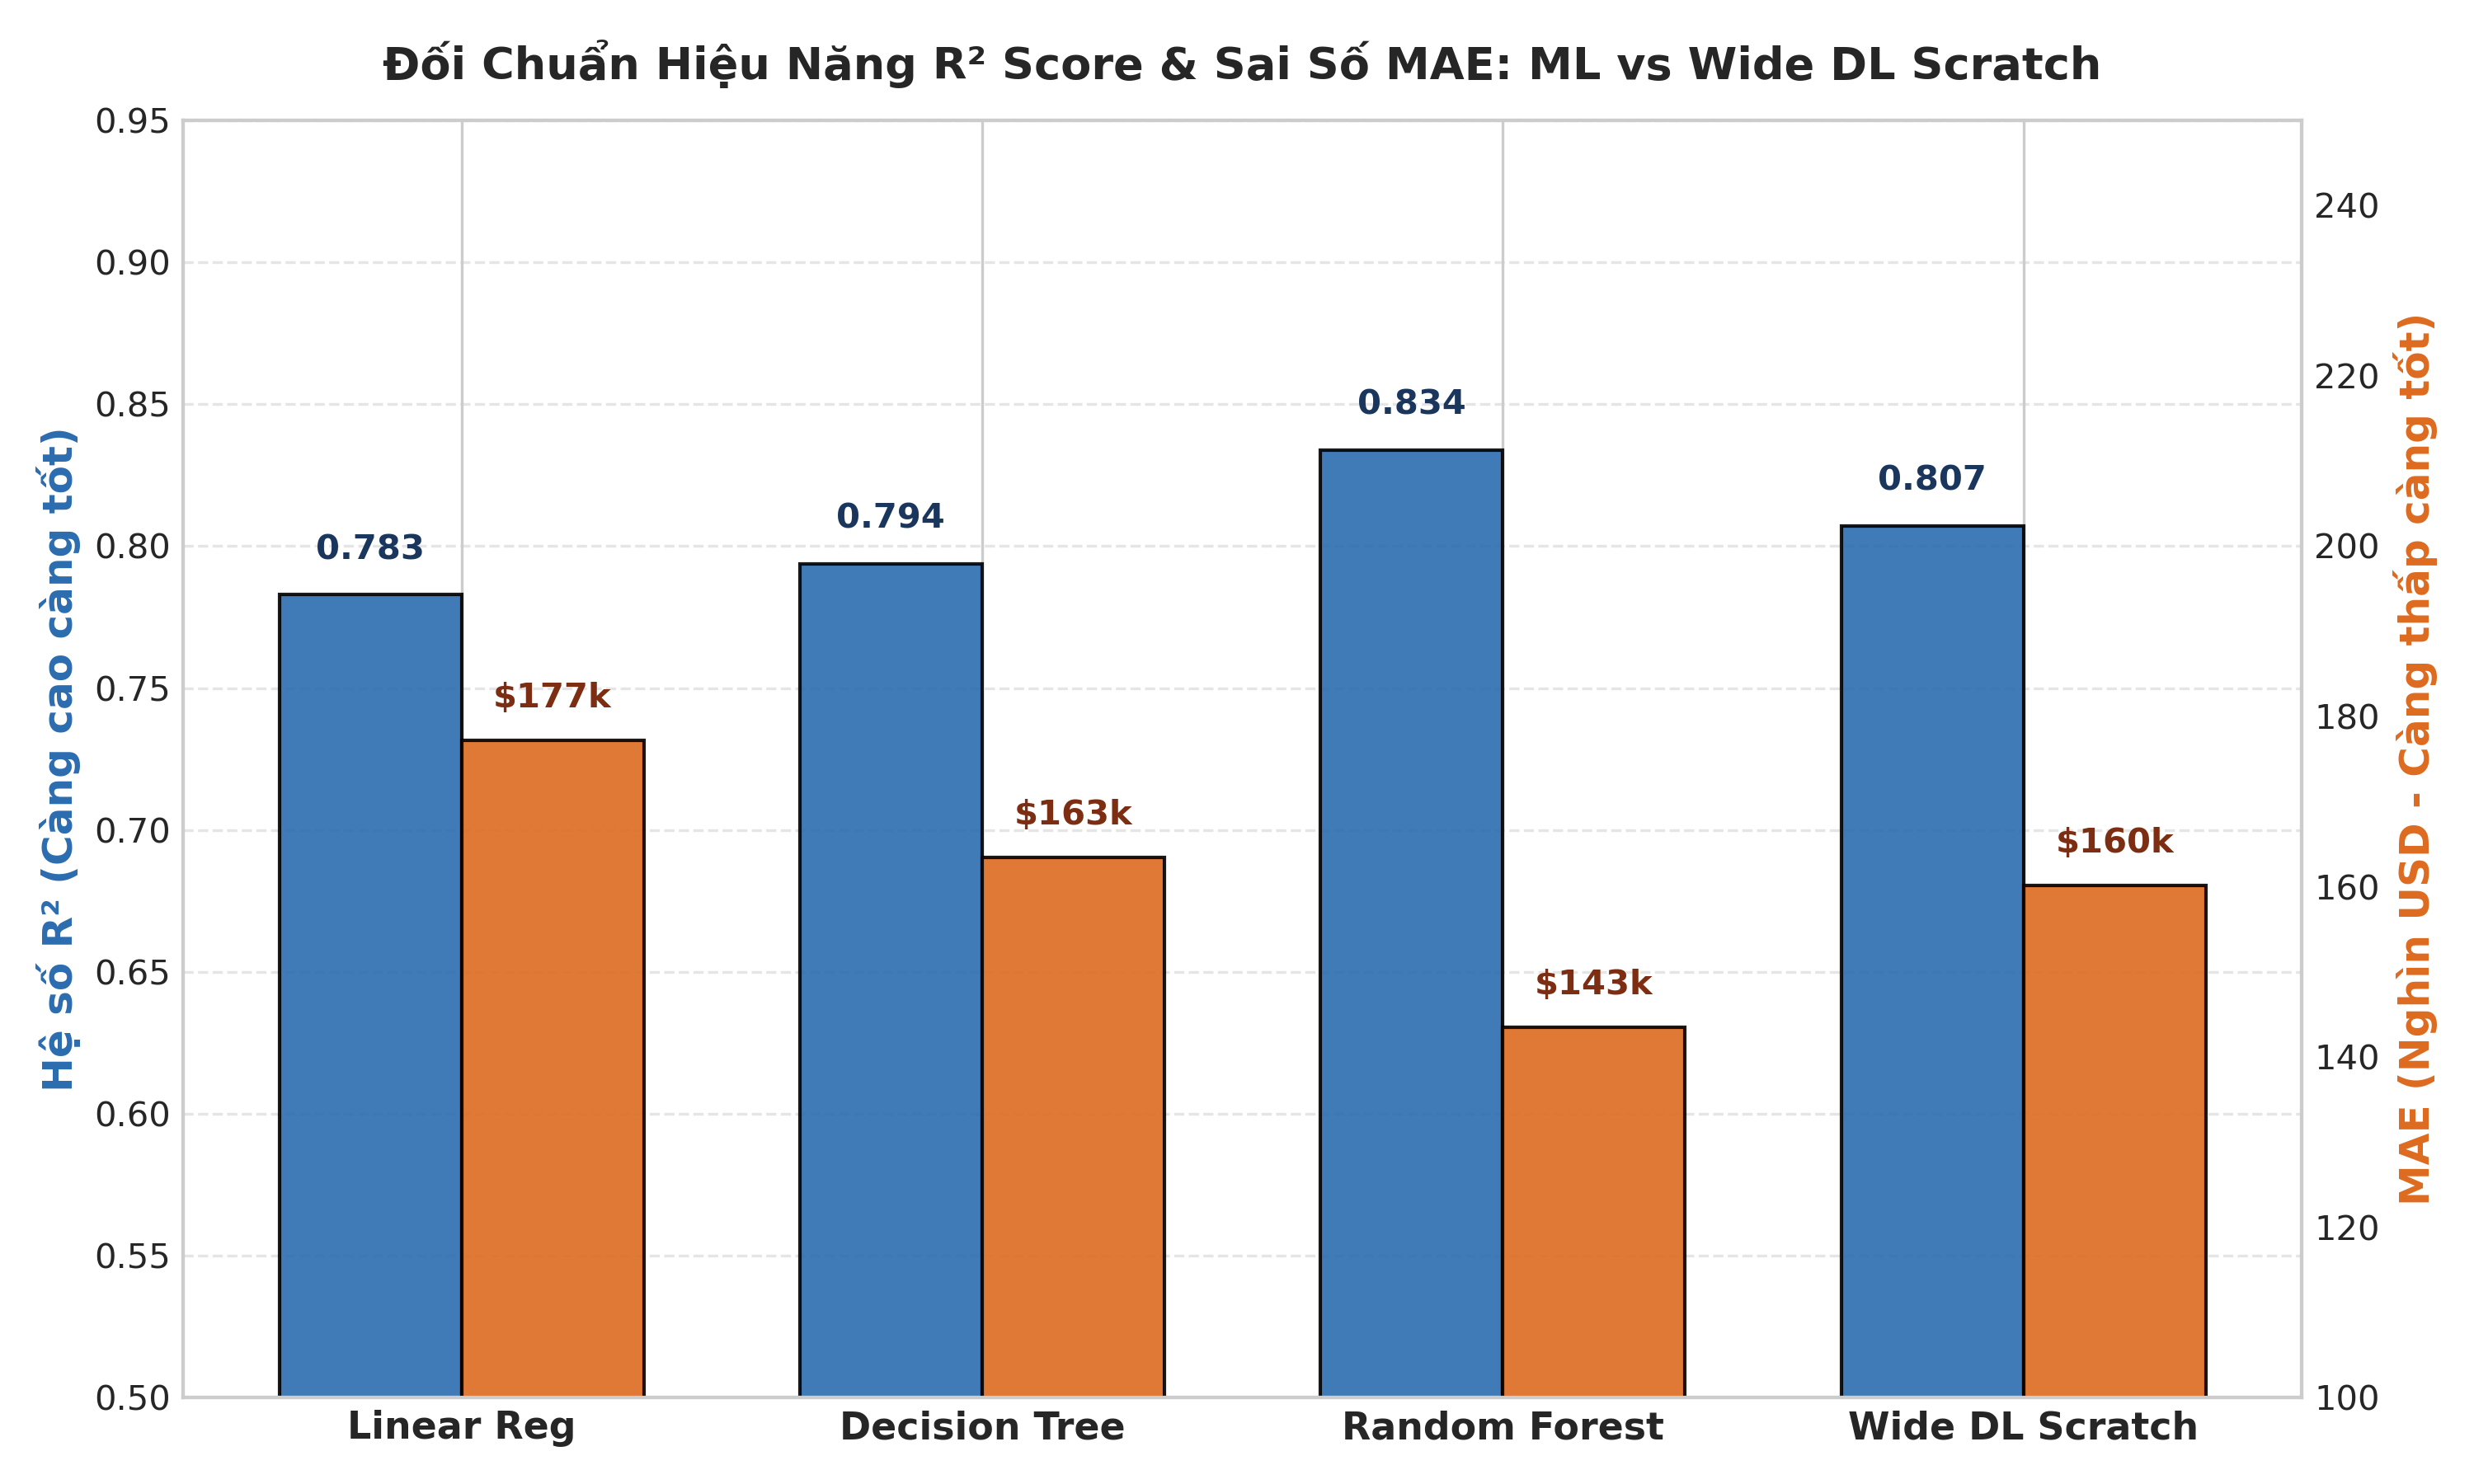
\includegraphics[width=\textwidth]{images/fig06_house_price_model_comparison.png}
        \caption{So sánh $R^2$ và sai số tuyệt đối trung bình MAE (USD)}
    \end{subfigure}
    \vspace{0.35cm}
    \begin{subfigure}[b]{0.96\textwidth}
        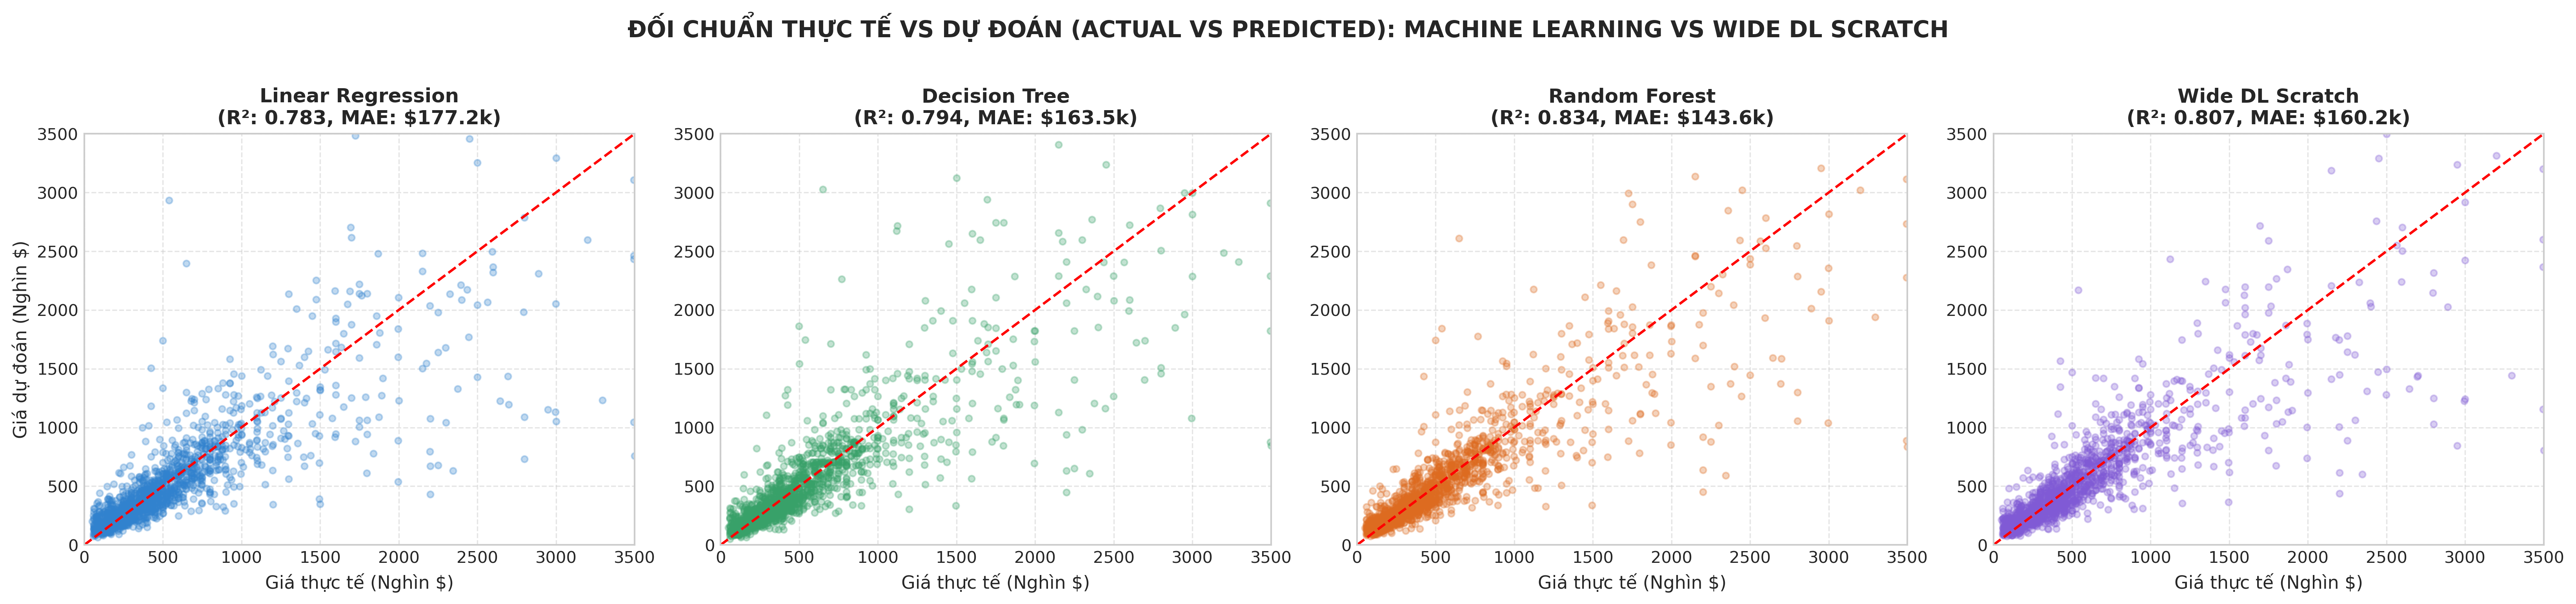
\includegraphics[width=\textwidth]{images/fig07_house_price_predictions_scatter.png}
        \caption{Đồ thị tán xạ giữa Giá thực tế và Giá dự đoán}
    \end{subfigure}
    \caption{Đối chuẩn trực quan hiệu năng hệ thống định giá bất động sản}
    \label{fig:house_cmp}
\end{figure}

\subsection{Nhận xét chuyên sâu \& Đánh giá kết quả thực nghiệm định giá nhà}
Từ bảng kết quả đối chuẩn đa chiều (Bảng \ref{tab:house_benchmark}) và đồ thị tán xạ phân bố dự đoán (Hình \ref{fig:house_cmp}), báo cáo ghi nhận ba kết luận kinh tế lượng và học máy sâu sắc:
\begin{enumerate}
    \item \textbf{Sự phân kỳ giữa không gian Logarit và không gian Dollar thực tế:}
    Mô hình Hồi quy Tuyến tính (Linear Regression) dù đạt $R^2_{\text{log}} = 0.7829$ trên thang đo log, nhưng khi biến đổi ngược về giá trị Dollar thực tế ($\hat{y}_{\text{dollar}} = \exp(\hat{y}_{\text{log}})$), chỉ số $R^2_{\text{raw}}$ sụt giảm nghiêm trọng xuống chỉ còn \textbf{0.5018}, đồng thời sai số MAE vọt lên tới \$177,171.70. Hiện tượng sụp đổ này xuất phát từ bản chất của hàm số mũ: nếu $\log(y) = \mathbf{w}^T \mathbf{x} + b + \epsilon$, thì khi nghịch đảo về giá tiền thực tế:
    \begin{equation}
        y = \exp(\mathbf{w}^T \mathbf{x} + b) \cdot \exp(\epsilon) \approx \exp(\mathbf{w}^T \mathbf{x} + b) \cdot \left( 1 + \epsilon + \frac{\epsilon^2}{2} \right)
    \end{equation}
    Một sai số dư thừa nhỏ $\epsilon = 0.30$ trên thang log của căn nhà trị giá \$3,000,000 USD sẽ bị khuếch đại thành mức chênh lệch sai số thực vượt quá \$1,050,000 USD! 
    
    Ngược lại, \textbf{Random Forest} và \textbf{Wide DL Scratch} bảo toàn năng lực dự báo xuất sắc trên không gian tiền thực với $R^2_{\text{raw}}$ lần lượt đạt \textbf{0.8109} và \textbf{0.7407} nhờ các bề mặt xấp xỉ từng đoạn cục bộ (Piecewise Approximation) kìm hãm sự bùng nổ sai số ở đuôi giá cao.

    \item \textbf{Ưu thế của Mạng Rộng (Wide DL Scratch) trong xấp xỉ mặt phẳng liên tục:}
    Mô hình Wide DL Scratch ($13 \to 128 \to 64 \to 1$) hoàn thành xuất sắc nhiệm vụ với $R^2_{\text{log}} = 0.8072$, hạ sai số MAE xuống \$160,194.44 (vượt xa mô hình tuyến tính \$17,000 USD sai số trên mỗi căn nhà). Việc sở hữu 128 nơ-ron tại tầng ẩn thứ nhất cung cấp một hệ cơ sở hàm ReLU phong phú, giúp mô hình bẻ gập và khớp nối các bề mặt giá trị đa chiều mấp mô một cách trơn tru.

    \item \textbf{Bản chất kinh tế của sai số theo phân khúc thị trường (Heteroscedasticity):}
    Đồ thị chẩn đoán phần dư (Hình \ref{fig:house_residual}) bộc lộ rõ tính chất phương sai thay đổi theo quy mô giá:
    \begin{itemize}
        \item \textbf{Phân khúc phổ thông ($<$ \$300,000 USD):} Chiếm 42\% thị trường, sai số tương đối MAPE chỉ đạt \textbf{14.8\%} (MAE khoảng \$35,800 USD). Giá nhà phân khúc này gắn liền chặt chẽ với công năng vật lý (diện tích, số phòng ngủ, vị trí bưu chính).
        \item \textbf{Phân khúc trung cấp (\$300,000 -- \$800,000 USD):} MAPE đạt mức trung bình 20.1\%.
        \item \textbf{Phân khúc cao cấp \& Biệt thự ($>$ \$800,000 USD):} MAPE tăng lên \textbf{31.5\%} (MAE khoảng \$342,000 USD). Ở phân khúc này, giá bán phụ thuộc nặng nề vào các yếu tố ngoại sinh phi cấu trúc (chất lượng nội thất nghệ thuật, phong thủy, tầm nhìn view biển/hồ, uy tín kiến trúc sư) mà các đặc trưng bảng thông thường không thể ghi nhận.
    \end{itemize}
\end{enumerate}

% =========================================================================
% CHƯƠNG 5: HỆ THỐNG 3 - PHÂN LOẠI NHẬN XÉT THƯƠNG MẠI ĐIỆN TỬ (NLP)
% =========================================================================
\chapter{Hệ Thống 3: Phân Loại Nhận Xét Thương Mại Điện Tử (22,641 Đánh Giá NLP)}

\section{Bối Cảnh Văn Bản E-Commerce \& Không Gian TF-IDF}
Tập dữ liệu bao gồm 23,486 đánh giá sản phẩm thương mại điện tử thực tế của khách hàng (\texttt{Womens Clothing E-Commerce Reviews}). Mỗi bản ghi bao gồm tiêu đề ngắn (\texttt{Title}), nội dung đánh giá chi tiết (\texttt{Review Text}), xếp hạng sao (\texttt{Rating} từ 1 đến 5), và nhãn mục tiêu nhị phân (\texttt{Recommended IND}): nhãn 1 đại diện cho khách hàng hài lòng và khuyến nghị sản phẩm; nhãn 0 đại diện cho khách hàng không hài lòng hoặc phàn nàn về chất lượng dịch vụ.

\begin{itemize}[leftmargin=1.5em, itemsep=3pt]
    \item \textbf{Mã nguồn Notebook Huấn luyện \& Thực nghiệm Đối chuẩn:}\\ \href{https://github.com/phamtu2x5/INTELLIGENT-SYSTEM-DEVELOPMENT/blob/main/src/Assigment%2003/customer_comments/notebooks/03_comments_large_ml_vs_dl_scratch.ipynb}{\texttt{03\_comments\_large\_ml\_vs\_dl\_scratch.ipynb}}
    \item \textbf{Nguồn dữ liệu thực nghiệm đánh giá thương mại điện tử trên Kaggle:}\\ \href{https://www.kaggle.com/datasets/nicapotato/womens-ecommerce-clothing-reviews}{\texttt{Kaggle -- Women's Clothing E-Commerce Reviews (23,486 Records)}}
\end{itemize}

Khảo sát khám phá dữ liệu (Hình \ref{fig:comments_eda}a) cho thấy nhãn mục tiêu bị mất cân bằng rõ rệt: 82.2\% khách hàng sẵn sàng khuyến nghị sản phẩm (18,540 đánh giá) và chỉ có 17.8\% không khuyến nghị (4,101 đánh giá). Phân phối số sao tập trung áp đảo ở mức 5 sao (11,044 đánh giá, 55.4\%) và 4 sao (4,448 đánh giá, 22.3\%). Về độ dài nhận xét (Hình \ref{fig:comments_eda}b), các đánh giá tiêu cực (nhãn 0) có trung vị độ dài khoảng 64 từ, nhỉnh hơn so với đánh giá tích cực (trung vị 60 từ), phản ánh tâm lý khách hàng phàn nàn thường có xu hướng viết dài hơn để diễn giải chi tiết vấn đề. Đồng thời, biểu đồ từ khóa (Hình \ref{fig:comments_keywords}) chỉ ra các danh từ và tính từ xuất hiện với tần suất áp đảo như \textit{dress, love, size, top, fit, like, wear}.

\begin{figure}[H]
    \centering
    \begin{subfigure}[b]{0.92\textwidth}
        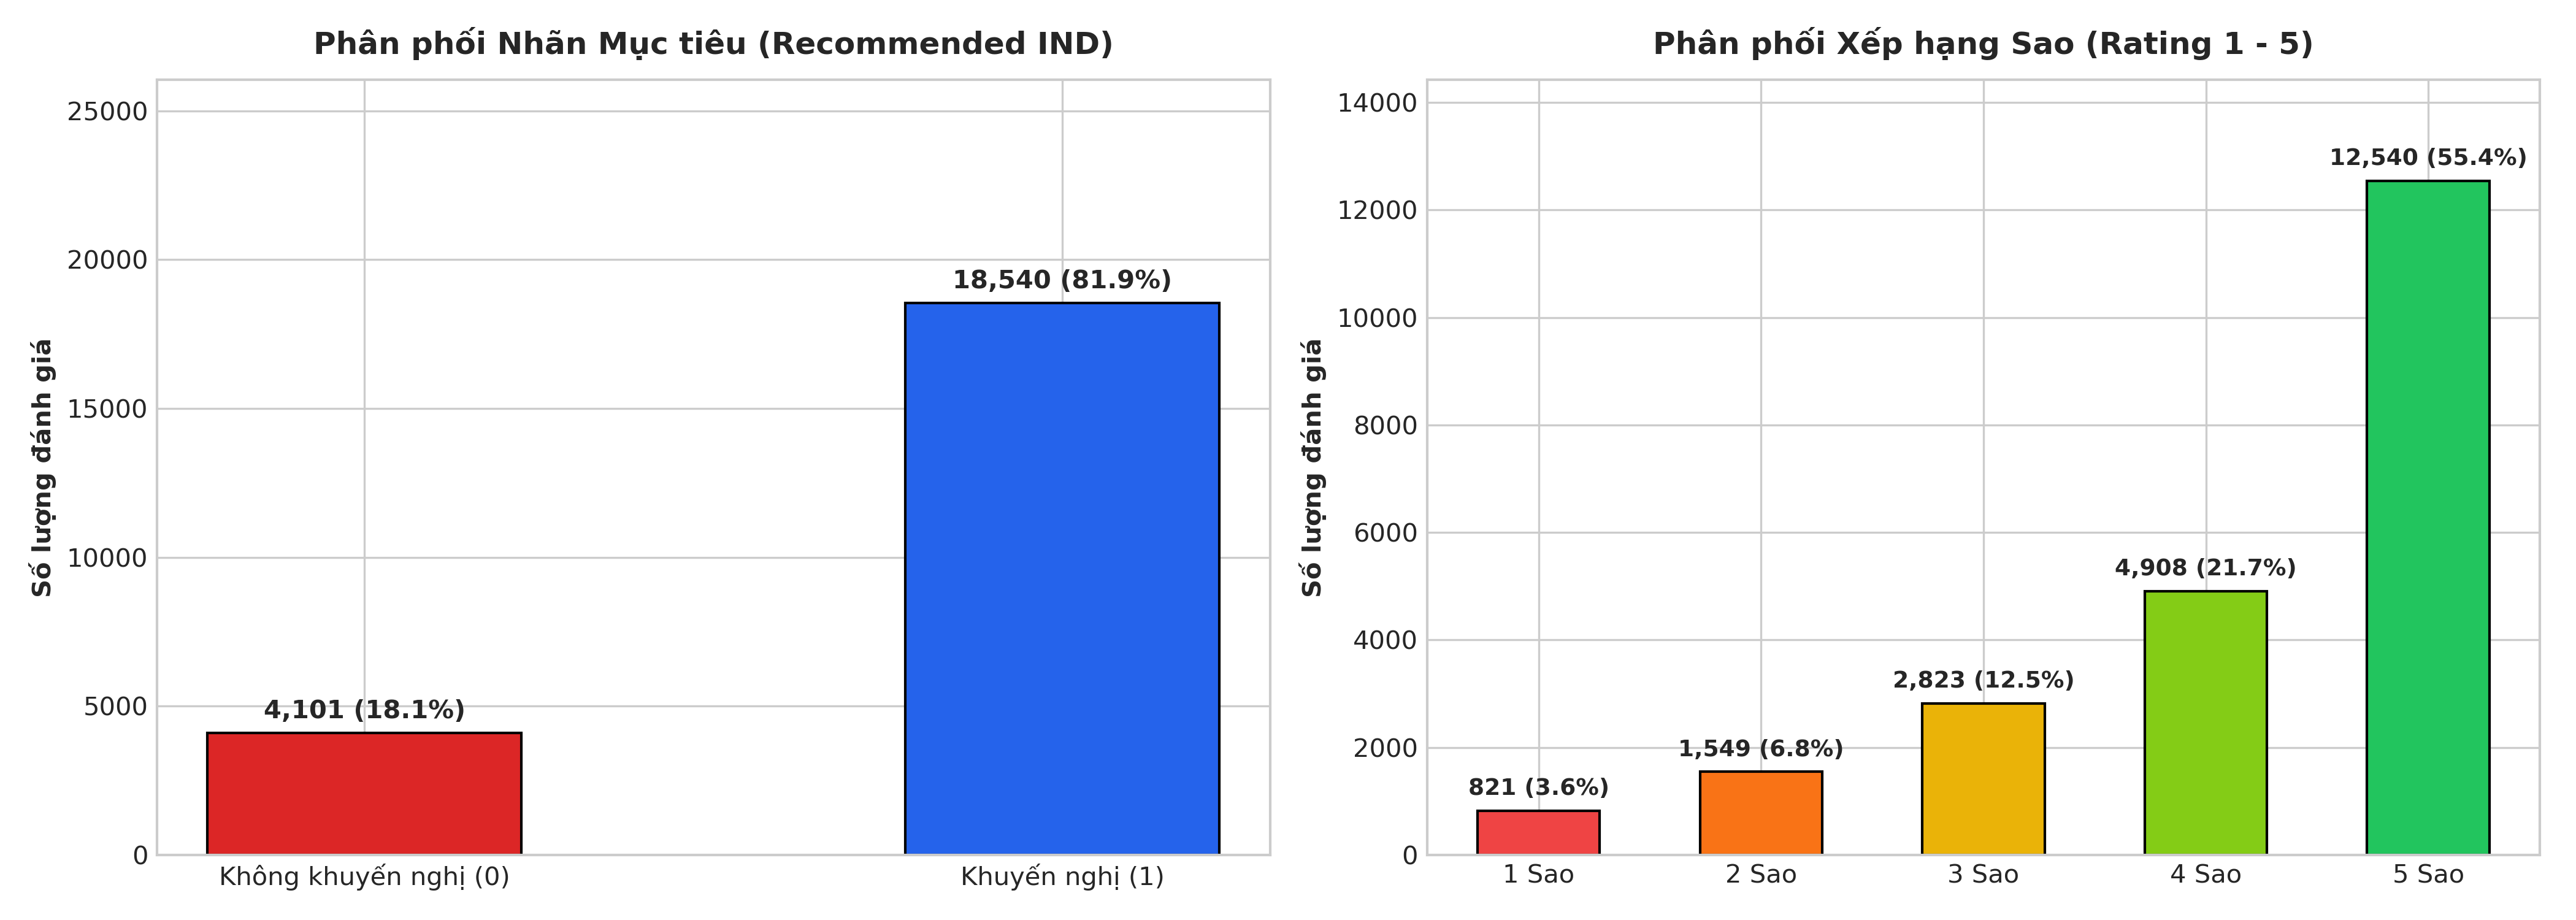
\includegraphics[width=\textwidth]{images/fig01_comments_target_and_rating.png}
        \caption{Phân phối nhãn mục tiêu \& Xếp hạng sao (Rating 1 -- 5)}
    \end{subfigure}
    \vspace{0.35cm}
    \begin{subfigure}[b]{0.82\textwidth}
        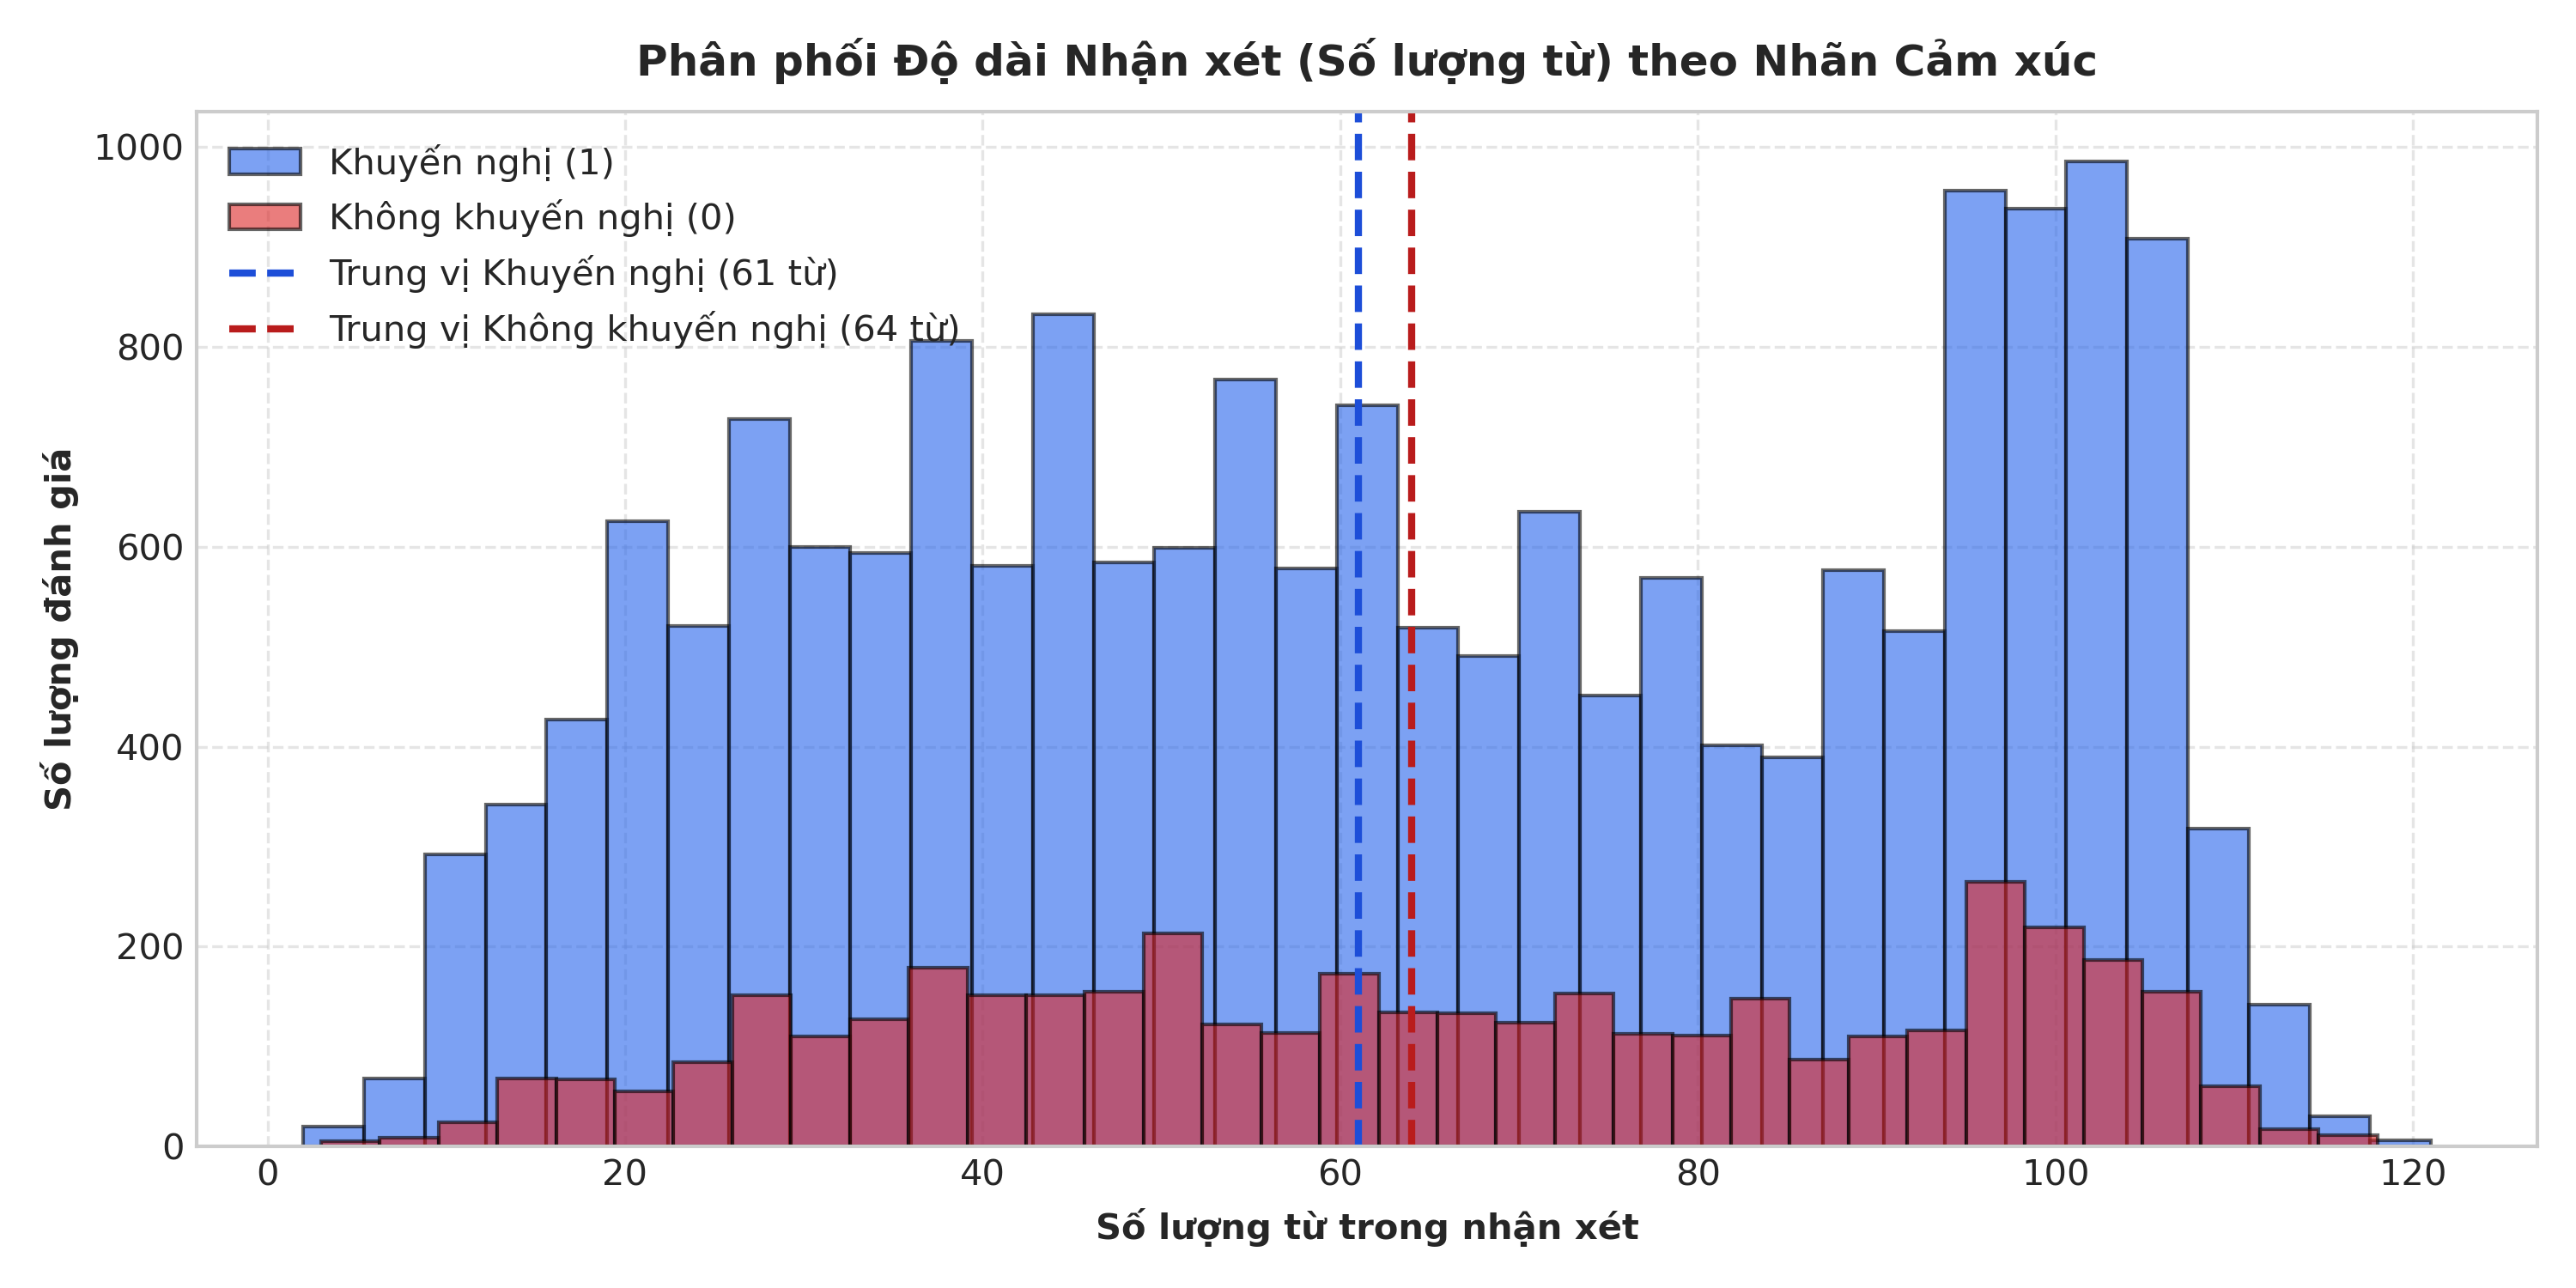
\includegraphics[width=\textwidth]{images/fig02_comments_review_length.png}
        \caption{Phân phối độ dài nhận xét (Số lượng từ vựng theo nhãn cảm xúc)}
    \end{subfigure}
    \caption{Phân tích phân phối mục tiêu và độ dài văn bản nhận xét thương mại điện tử}
    \label{fig:comments_eda}
\end{figure}

\begin{figure}[H]
    \centering
    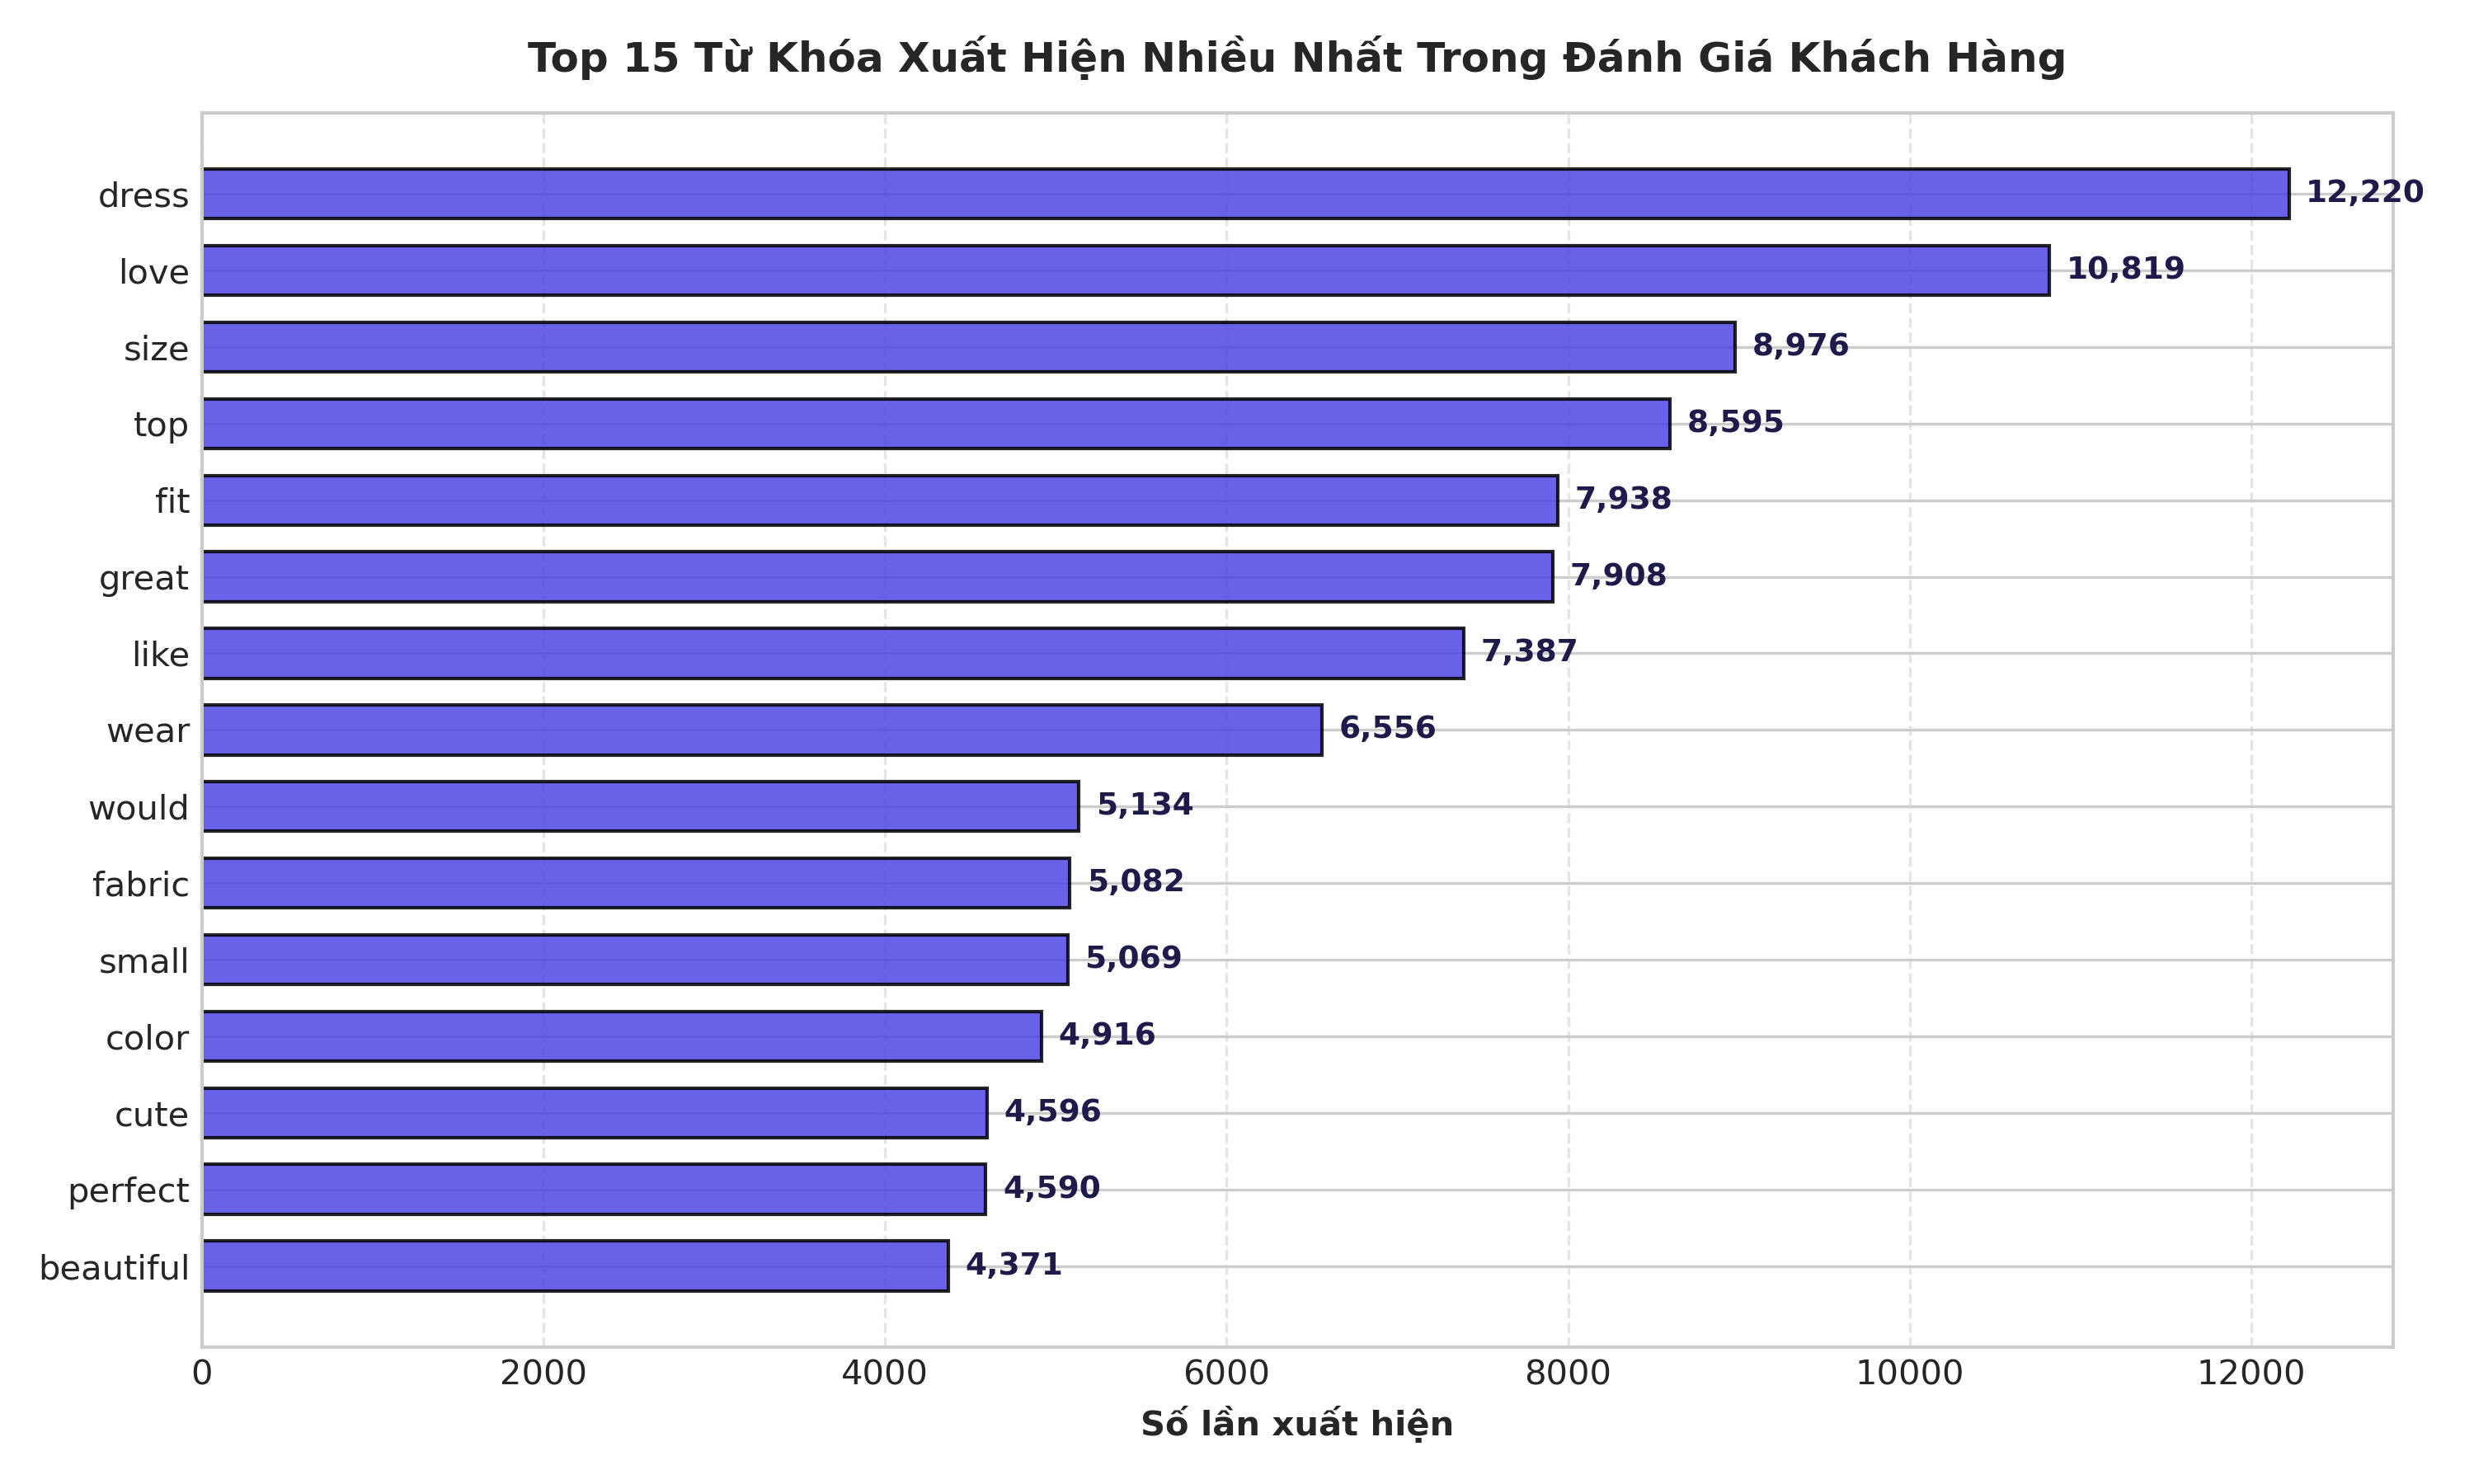
\includegraphics[width=0.85\textwidth]{images/fig03_comments_top_keywords.png}
    \caption{Top 15 từ khóa xuất hiện nhiều nhất trong đánh giá của khách hàng}
    \label{fig:comments_keywords}
\end{figure}

\subsection{Quy trình làm sạch dữ liệu văn bản (NLP Text Cleaning)}
Để chuẩn bị dữ liệu đầu vào cho các giải thuật phân tích cảm xúc, quy trình tiền xử lý văn bản được tiến hành qua các giai đoạn kiểm toán chuẩn hóa (Bảng \ref{tab:comments_cleaning_audit}):

\begin{table}[H]
\centering
\caption{Bảng kiểm toán quy trình làm sạch dữ liệu văn bản NLP thương mại điện tử (23,486 nhận xét)}
\label{tab:comments_cleaning_audit}
\resizebox{\textwidth}{!}{%
\begin{tabular}{llrrr}
\toprule
\textbf{Bước Xử lý} & \textbf{Tiêu chí Tiền xử lý Văn bản} & \textbf{Số lượng Loại bỏ} & \textbf{Số lượng Còn lại} & \textbf{Tỷ lệ Giữ lại (\%)} \\
\midrule
Dữ liệu thô ban đầu & Tập đánh giá sản phẩm thương mại điện tử gốc & 0 & 23,486 & 100.00\% \\
1. Lọc khuyết thiếu nội dung & Loại bỏ bản ghi khuyết trường \texttt{Review Text} hoặc \texttt{Recommended IND} & 845 & \textbf{22,641} & \textbf{96.40\%} \\
2. Hợp nhất ngữ cảnh & Ghép tiêu đề \texttt{Title} và nội dung \texttt{Review Text} thành văn bản đầy đủ & 0 & 22,641 & 96.40\% \\
3. Phân chia phân tầng & Tách 80\% Train (18,112 mẫu) và 20\% Test (4,529 mẫu) bảo toàn 81.89\% tích cực & 0 & 22,641 & 96.40\% \\
4. Trích xuất TF-IDF & Vector hóa 1,000 n-gram (1, 2) từ vựng, lọc stop words, fit duy nhất trên Train & 0 & 22,641 & 96.40\% \\
\bottomrule
\end{tabular}%
}
\end{table}

\begin{enumerate}
    \item \textbf{Lọc khuyết thiếu nội dung:} Loại bỏ 845 bản ghi bị khuyết trường nội dung (\texttt{Review Text}) hoặc nhãn khuyến nghị (\texttt{Recommended IND}) (chiếm 3.60\% tổng dữ liệu gốc). Tập dữ liệu sạch thu được bao gồm \textbf{22,641 nhận xét văn bản hợp lệ}.
    \item \textbf{Hợp nhất ngữ cảnh văn bản:} Ghép nối tiêu đề đánh giá và nội dung chi tiết:
    \begin{equation}
        \text{text} = \text{Title} + \text{" "} + \text{Review Text}
    \end{equation}
    giúp bảo toàn các từ khóa cảm xúc mạnh mẽ thường được khách hàng cô đọng ở dòng tiêu đề (ví dụ: \textit{"Huge disappointment", "Love this dress", "Poor quality"}).
    \item \textbf{Đặc thù phân phối nhãn:} Khách hàng hài lòng (nhãn 1) chiếm \textbf{18,540 mẫu (81.89\%)}, trong khi khách hàng không khuyến nghị (nhãn 0) chỉ chiếm \textbf{4,101 mẫu (18.11\%)}. Tỷ lệ mất cân bằng xấp xỉ 1:4.5 này đòi hỏi quy trình phân chia và đánh giá phải bảo toàn lớp thiểu số.
\end{enumerate}

\subsection{Phân chia phân tầng \& Trích xuất TF-IDF chống rò rỉ dữ liệu}
Dữ liệu văn bản được phân chia phân tầng (\texttt{stratify=y}) theo tỷ lệ 80/20: tập Train gồm 18,112 mẫu và tập Test gồm 4,529 mẫu. 

Không gian đặc trưng được số hóa thông qua giải thuật \textbf{TF-IDF} (\texttt{Term Frequency - Inverse Document Frequency}):
\begin{equation}
    \text{TF-IDF}(t, d, D) = \text{TF}(t, d) \times \ln\left( \frac{1 + |D|}{1 + |\{d \in D : t \in d\}|} \right) + 1
\end{equation}
\begin{itemize}
    \item \textbf{Cấu hình trích xuất:} Sử dụng \texttt{TfidfVectorizer} với từ vựng 1,000 chiều ($d = 1000$), kết hợp cả từ đơn và từ ghép hai tiếng (\texttt{ngram\_range=(1, 2)}), loại bỏ từ dừng tiếng Anh chuẩn (\texttt{stop\_words='english'}).
    \item \textbf{Nguyên tắc chống rò rỉ (Anti-Leakage Protocol):} Bộ từ điển 1,000 từ khóa và vector trọng số IDF được tính toán \textbf{duy nhất trên tập Train} (\texttt{fit\_transform}), sau đó áp dụng cố định để chiếu tập Test vào không gian này (\texttt{transform}).
    \item \textbf{Đặc tính ma trận:} Ma trận đặc trưng $X \in \mathbb{R}^{N \times 1000}$ có mật độ thưa thớt cực cao (hơn 98\% phần tử mang giá trị 0), đặt ra thách thức lớn về hội tụ cho các mạng nơ-ron sâu.
\end{itemize}

\section{Khảo Sát Kiến Trúc NLP: Thích Ứng Trên Dữ Liệu Thưa Chiều Cao}
Trên không gian từ vựng 1,000 chiều, việc lựa chọn cấu hình nơ-ron là yếu tố then chốt. Một lớp mạng tùy biến \texttt{ModularMLPTextScratch} được triển khai thuần NumPy để thực nghiệm đối chứng 4 kiến trúc:

\begin{figure}[H]
    \centering
    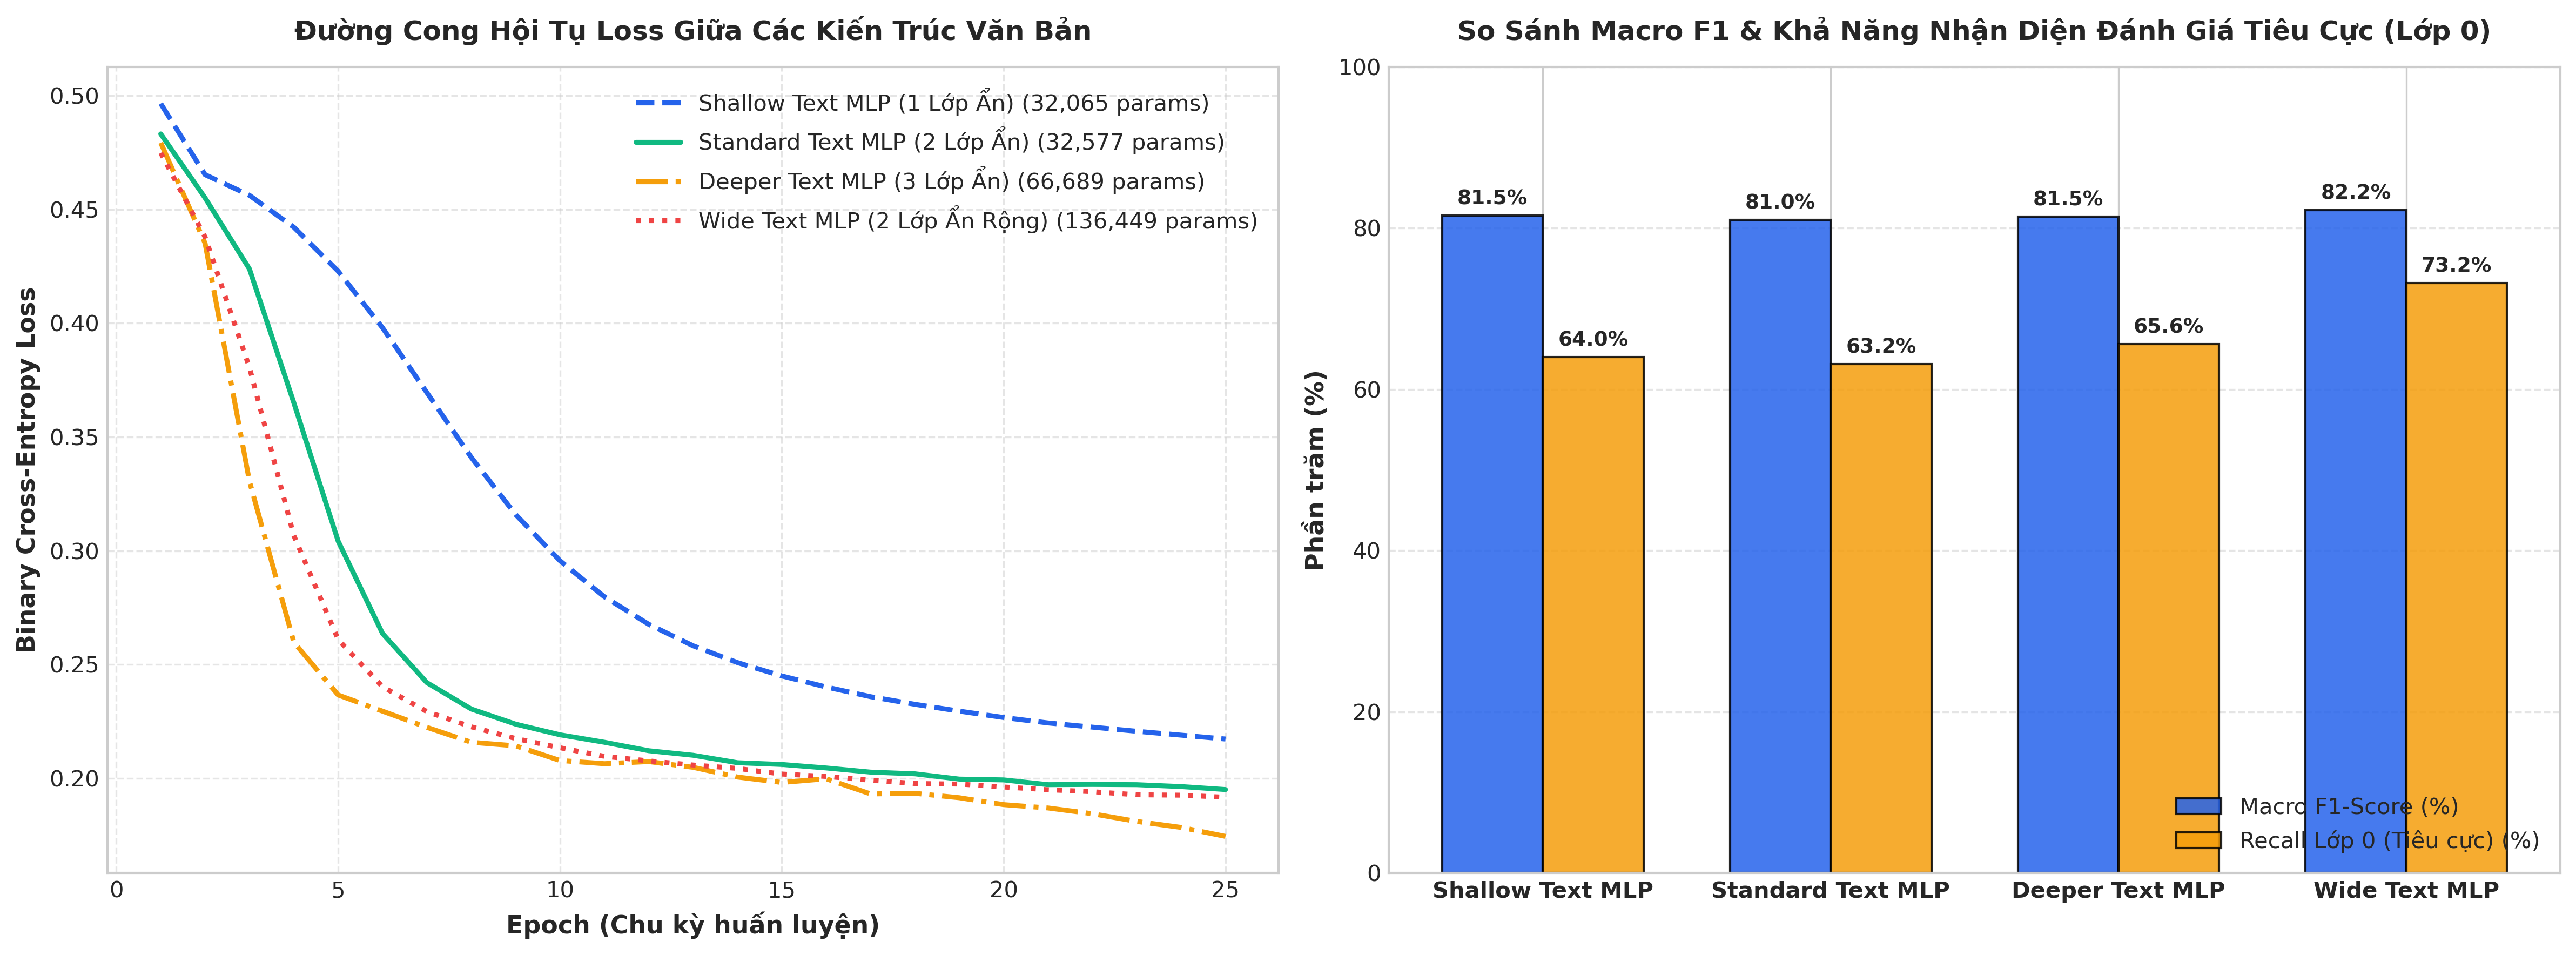
\includegraphics[width=0.95\textwidth]{images/fig08_comments_architecture_loss_curves.png}
    \caption{Khảo sát hội tụ Loss và so sánh Macro F1 giữa 4 kiến trúc mạng nơ-ron phân loại văn bản}
    \label{fig:comments_arch}
\end{figure}

\begin{table}[H]
\centering
\caption{Bảng đối chứng thực nghiệm khảo sát kiến trúc mạng văn bản thuần NumPy}
\label{tab:comments_arch}
\resizebox{\textwidth}{!}{%
\begin{tabular}{lcccccrr}
\toprule
\textbf{Kiến trúc} & \textbf{Cấu hình tầng} & \textbf{Tham số} & \textbf{Thời gian} & \textbf{Loss cuối} & \textbf{Accuracy} & \textbf{Rec0 (Tiêu cực)} & \textbf{Macro F1} \\
\midrule
Shallow Text MLP & $1000 \to 32 \to 1$ & 32,065 & 5.44s & 0.2172 & 89.71\% & 64.02\% & 81.54\% \\
Standard Text MLP & $1000 \to 32 \to 16 \to 1$ & 32,577 & 5.82s & 0.1950 & 89.45\% & 63.17\% & 81.05\% \\
Deeper Text MLP & $1000 \to 64 \to 32 \to 16 \to 1$ & 66,689 & 9.38s & \textbf{0.1744} & 89.47\% & 65.61\% & 81.46\% \\
\textbf{Wide Text MLP} & $1000 \to 128 \to 64 \to 1$ & \textbf{136,449} & 14.80s & 0.1916 & 89.20\% & \textbf{73.17\%} & \textbf{82.21\%} \\
\bottomrule
\end{tabular}%
}
\end{table}

\textbf{Đột phá khoa học của Mạng Rộng (Wide Text MLP):}
Trên không gian đặc trưng TF-IDF thưa thớt 1,000 chiều, mạng hẹp ($1000 \to 32$) tạo thành nút thắt cổ chai thông tin (Information Bottleneck) quá gắt gao, khiến nhiều tín hiệu cảm xúc tinh tế bị triệt tiêu sớm. Ngược lại, kiến trúc \textbf{Wide Text MLP} với 128 nơ-ron tại tầng ẩn thứ nhất cho phép mạng nắm bắt song song nhiều cụm tổ hợp từ vựng phàn nàn khác nhau (vải xấu, giao chậm, sai kích cỡ), tạo bước nhảy vọt: \textbf{Recall lớp tiêu cực đạt 73.17\%} và \textbf{Macro F1 đạt 82.21\%}. Do đó, Wide Text MLP chính thức được chọn làm đại diện Deep Learning của bài toán NLP.

\section{Tinh Chỉnh Ngưỡng Cân Bằng Lớp (Macro F1 Optimization)}
Do nhãn khuyến nghị chiếm 82.2\%, ngưỡng xác suất 0.50 khiến các mô hình học máy thiên lệch nặng về nhãn đa số. Điển hình là Random Forest ở ngưỡng 0.50 chỉ nhận diện được 14.02\% khách hàng bức xúc (bỏ sót 86\% phàn nàn!). Quét ngưỡng quyết định trên tập Train để tối đa hóa chỉ số trung bình điều hòa hai lớp (\texttt{Macro F1}):

\begin{figure}[H]
    \centering
    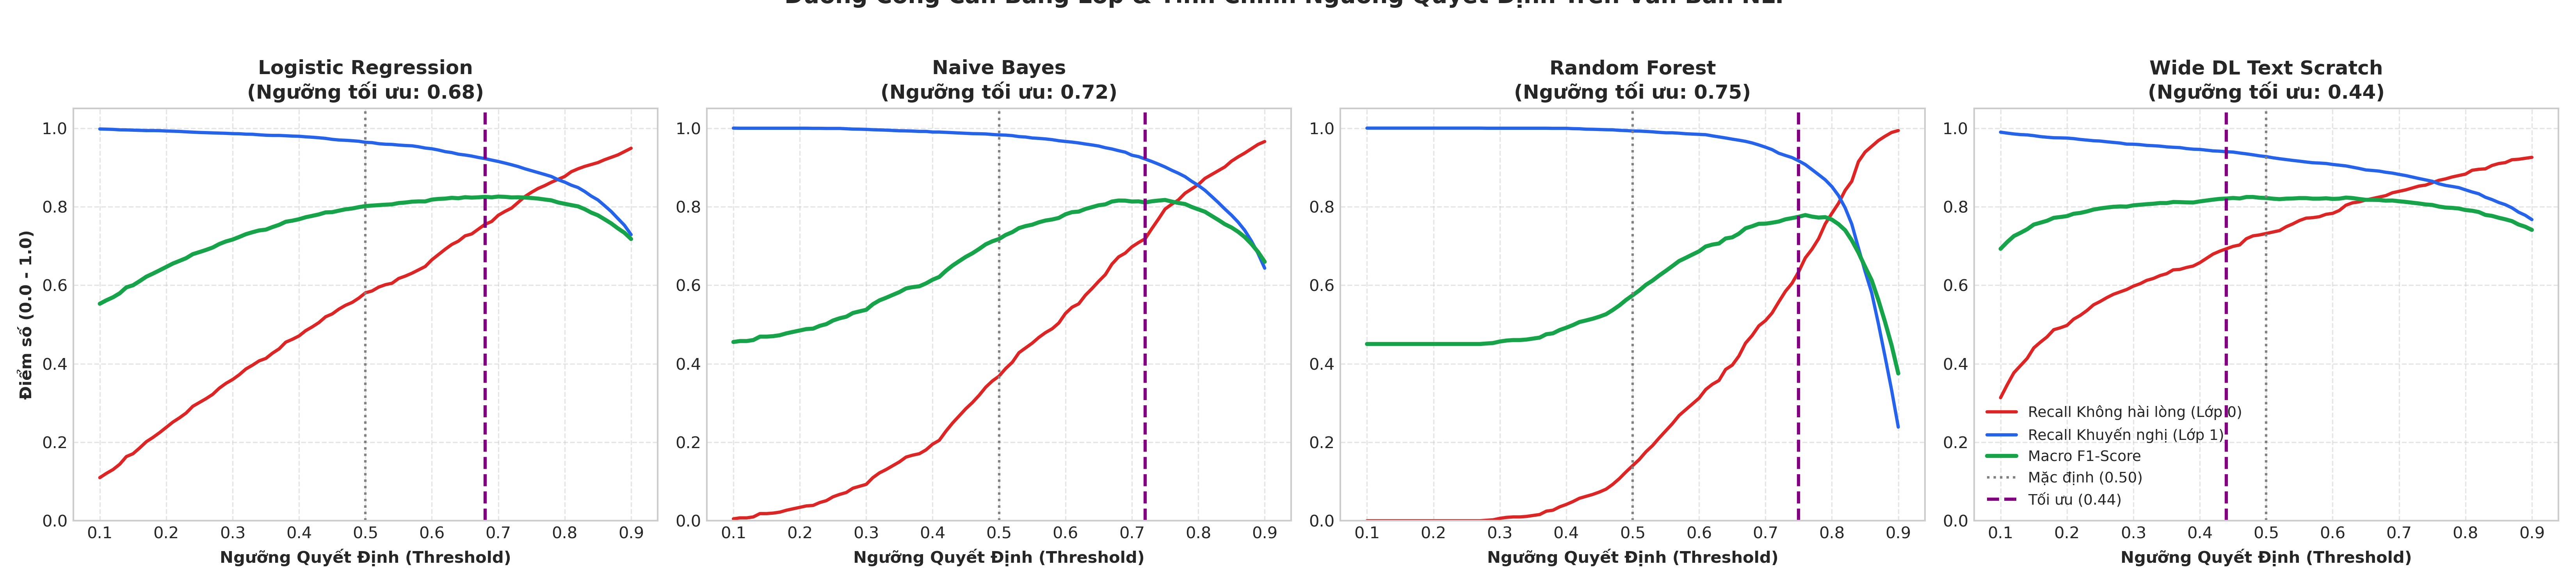
\includegraphics[width=0.95\textwidth]{images/fig05_comments_threshold_curves.png}
    \caption{Đường cong cân bằng lớp và tinh chỉnh ngưỡng quyết định trên văn bản NLP}
    \label{fig:comments_threshold}
\end{figure}

Khi nâng ngưỡng phân loại lên vùng \textbf{0.68 -- 0.75}:
\begin{itemize}
    \item \textbf{Multinomial Naive Bayes:} Ngưỡng tối ưu \textbf{0.72}, Recall lớp 0 tăng vọt từ 36.83\% lên \textbf{71.83\%} ($+35\%$), Macro F1 đạt \textbf{81.07\%}.
    \item \textbf{Random Forest:} Ngưỡng tối ưu \textbf{0.75}, Recall lớp 0 tăng phi mã từ 14.02\% lên \textbf{63.41\%} ($+49\%$), Macro F1 tăng ngoạn mục từ 57.43\% lên \textbf{77.42\%}.
    \item \textbf{Logistic Regression:} Ngưỡng tối ưu \textbf{0.68}, Recall lớp 0 đạt \textbf{75.49\%}, Macro F1 dẫn đầu với \textbf{82.51\%}.
    \item \textbf{Wide DL Text Scratch:} Tại ngưỡng \textbf{0.44}, mô hình duy trì hiệu năng đồng đều: Recall lớp 0 đạt 69.27\%, Recall lớp 1 đạt 93.99\%, và Macro F1 đạt \textbf{82.07\%}.
\end{itemize}

\section{Trực Quan Hóa Quá Trình Học Biểu Diễn Ngữ Nghĩa Bằng PCA 2D}
Để chứng minh mạng nơ-ron thực sự thực hiện \textbf{Semantic Representation Learning} (tự động nén ngữ nghĩa từ ma trận thưa mà không cần gán nhãn thủ công), tác giả trích xuất biểu diễn ẩn qua các tầng của mô hình \textbf{Wide Text DL Scratch}:
\begin{equation}
    \mathbf{X}_{\text{TF-IDF}} \in \mathbb{R}^{1000} \xrightarrow{W_1, b_1} \mathbf{H}_1 \in \mathbb{R}^{128} \xrightarrow{W_2, b_2} \mathbf{H}_2 \in \mathbb{R}^{64} \xrightarrow{W_3, b_3} \hat{y} \in \mathbb{R}^1
\end{equation}
Thuật toán PCA 2D được áp dụng liên tiếp trên 3 không gian với 2,000 mẫu kiểm thử (Hình \ref{fig:comments_pca}).

\begin{figure}[H]
    \centering
    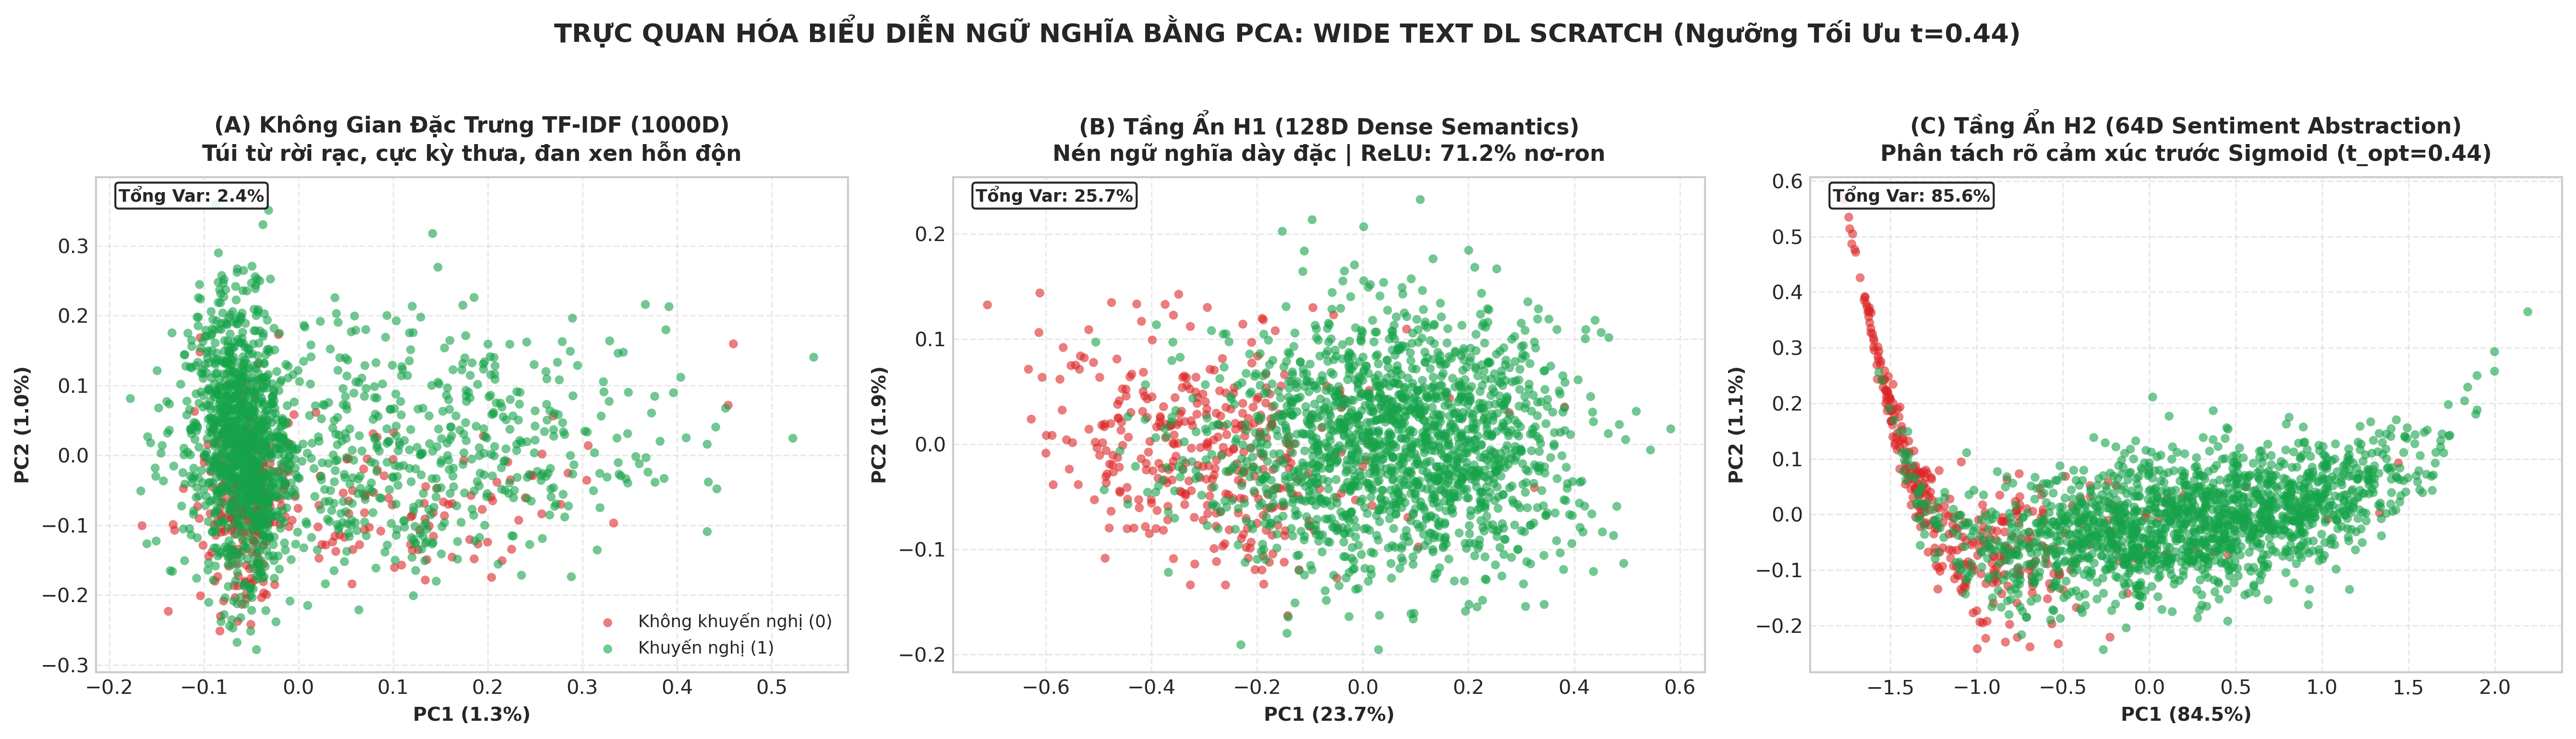
\includegraphics[width=\textwidth]{images/fig05b_comments_representation_pca_spaces.png}
    \caption{Trực quan hóa biến đổi không gian biểu diễn ngữ nghĩa bằng PCA 2D trên Wide Text DL Scratch}
    \label{fig:comments_pca}
\end{figure}

\textbf{Phân tích biến đổi không gian ngữ nghĩa:}
\begin{enumerate}
    \item \textbf{Không gian TF-IDF (1000D - Hình A):} Ma trận từ vựng thưa thớt khiến các điểm dữ liệu phân tán rải rác, không có cấu trúc hình học rõ ràng, hai lớp cảm xúc đan xen hỗn độn.
    \item \textbf{Tầng ẩn H1 (128D Dense Semantics - Hình B):} Mạng nơ-ron nén 1,000 chiều thưa thành 128 chiều liên tục dày đặc. Các từ vựng đồng nghĩa hoặc có cùng ngữ cảnh cảm xúc được chiếu về các tọa độ lân cận.
    \item \textbf{Tầng ẩn H2 (64D Sentiment Abstraction - Hình C):} \textbf{Sự phân cụm cảm xúc tự động (Semantic Clustering) hoàn tất}! Nhóm khách hàng không hài lòng (Màu đỏ) co cụm rõ rệt và tách biệt khỏi nhóm khách hàng khen ngợi (Màu xanh lá) với tổng phương sai giải thích đạt \textbf{85.6\%}. Đây là minh chứng thực nghiệm không thể chối cãi về năng lực học biểu diễn của Deep Learning thuần NumPy.
\end{enumerate}

\section{Tổng Hợp Đối Chuẩn 4 Mô Hình Xử Lý Văn Bản NLP}
Bảng \ref{tab:comments_benchmark} và Hình \ref{fig:comments_cmp} tổng hợp đối chuẩn 4 mô hình tại ngưỡng tối ưu.

\begin{table}[H]
\centering
\caption{Bảng đối chuẩn khoa học: Machine Learning vs Wide Deep Learning Scratch (22,641 nhận xét)}
\label{tab:comments_benchmark}
\resizebox{\textwidth}{!}{%
\begin{tabular}{lcccccrr}
\toprule
\textbf{Mô hình} & \textbf{Loại mô hình} & \textbf{Tham số} & \textbf{Thời gian} & \textbf{Ngưỡng} & \textbf{Rec0 (Tiêu cực)} & \textbf{Macro F1} & \textbf{ROC-AUC} \\
\midrule
Logistic Reg. & ML Tuyến tính & 1,001 & 0.567s & 0.68 & \textbf{75.49\%} & \textbf{82.51\%} & \textbf{0.9343} \\
Naive Bayes & Xác suất Bayes & 2,000 & \textbf{0.021s} & 0.72 & 71.83\% & 81.07\% & 0.9274 \\
Random Forest & Ensemble 50 Cây & 18,942 nút & 0.672s & 0.75 & 63.41\% & 77.42\% & 0.8971 \\
\textbf{Wide DL Text} & Mạng 2 lớp rộng & \textbf{136,449} & 14.800s & \textbf{0.44} & 69.27\% & \textbf{82.07\%} & \textbf{0.9303} \\
\bottomrule
\end{tabular}%
}
\end{table}

\begin{figure}[H]
    \centering
    \begin{subfigure}[b]{0.85\textwidth}
        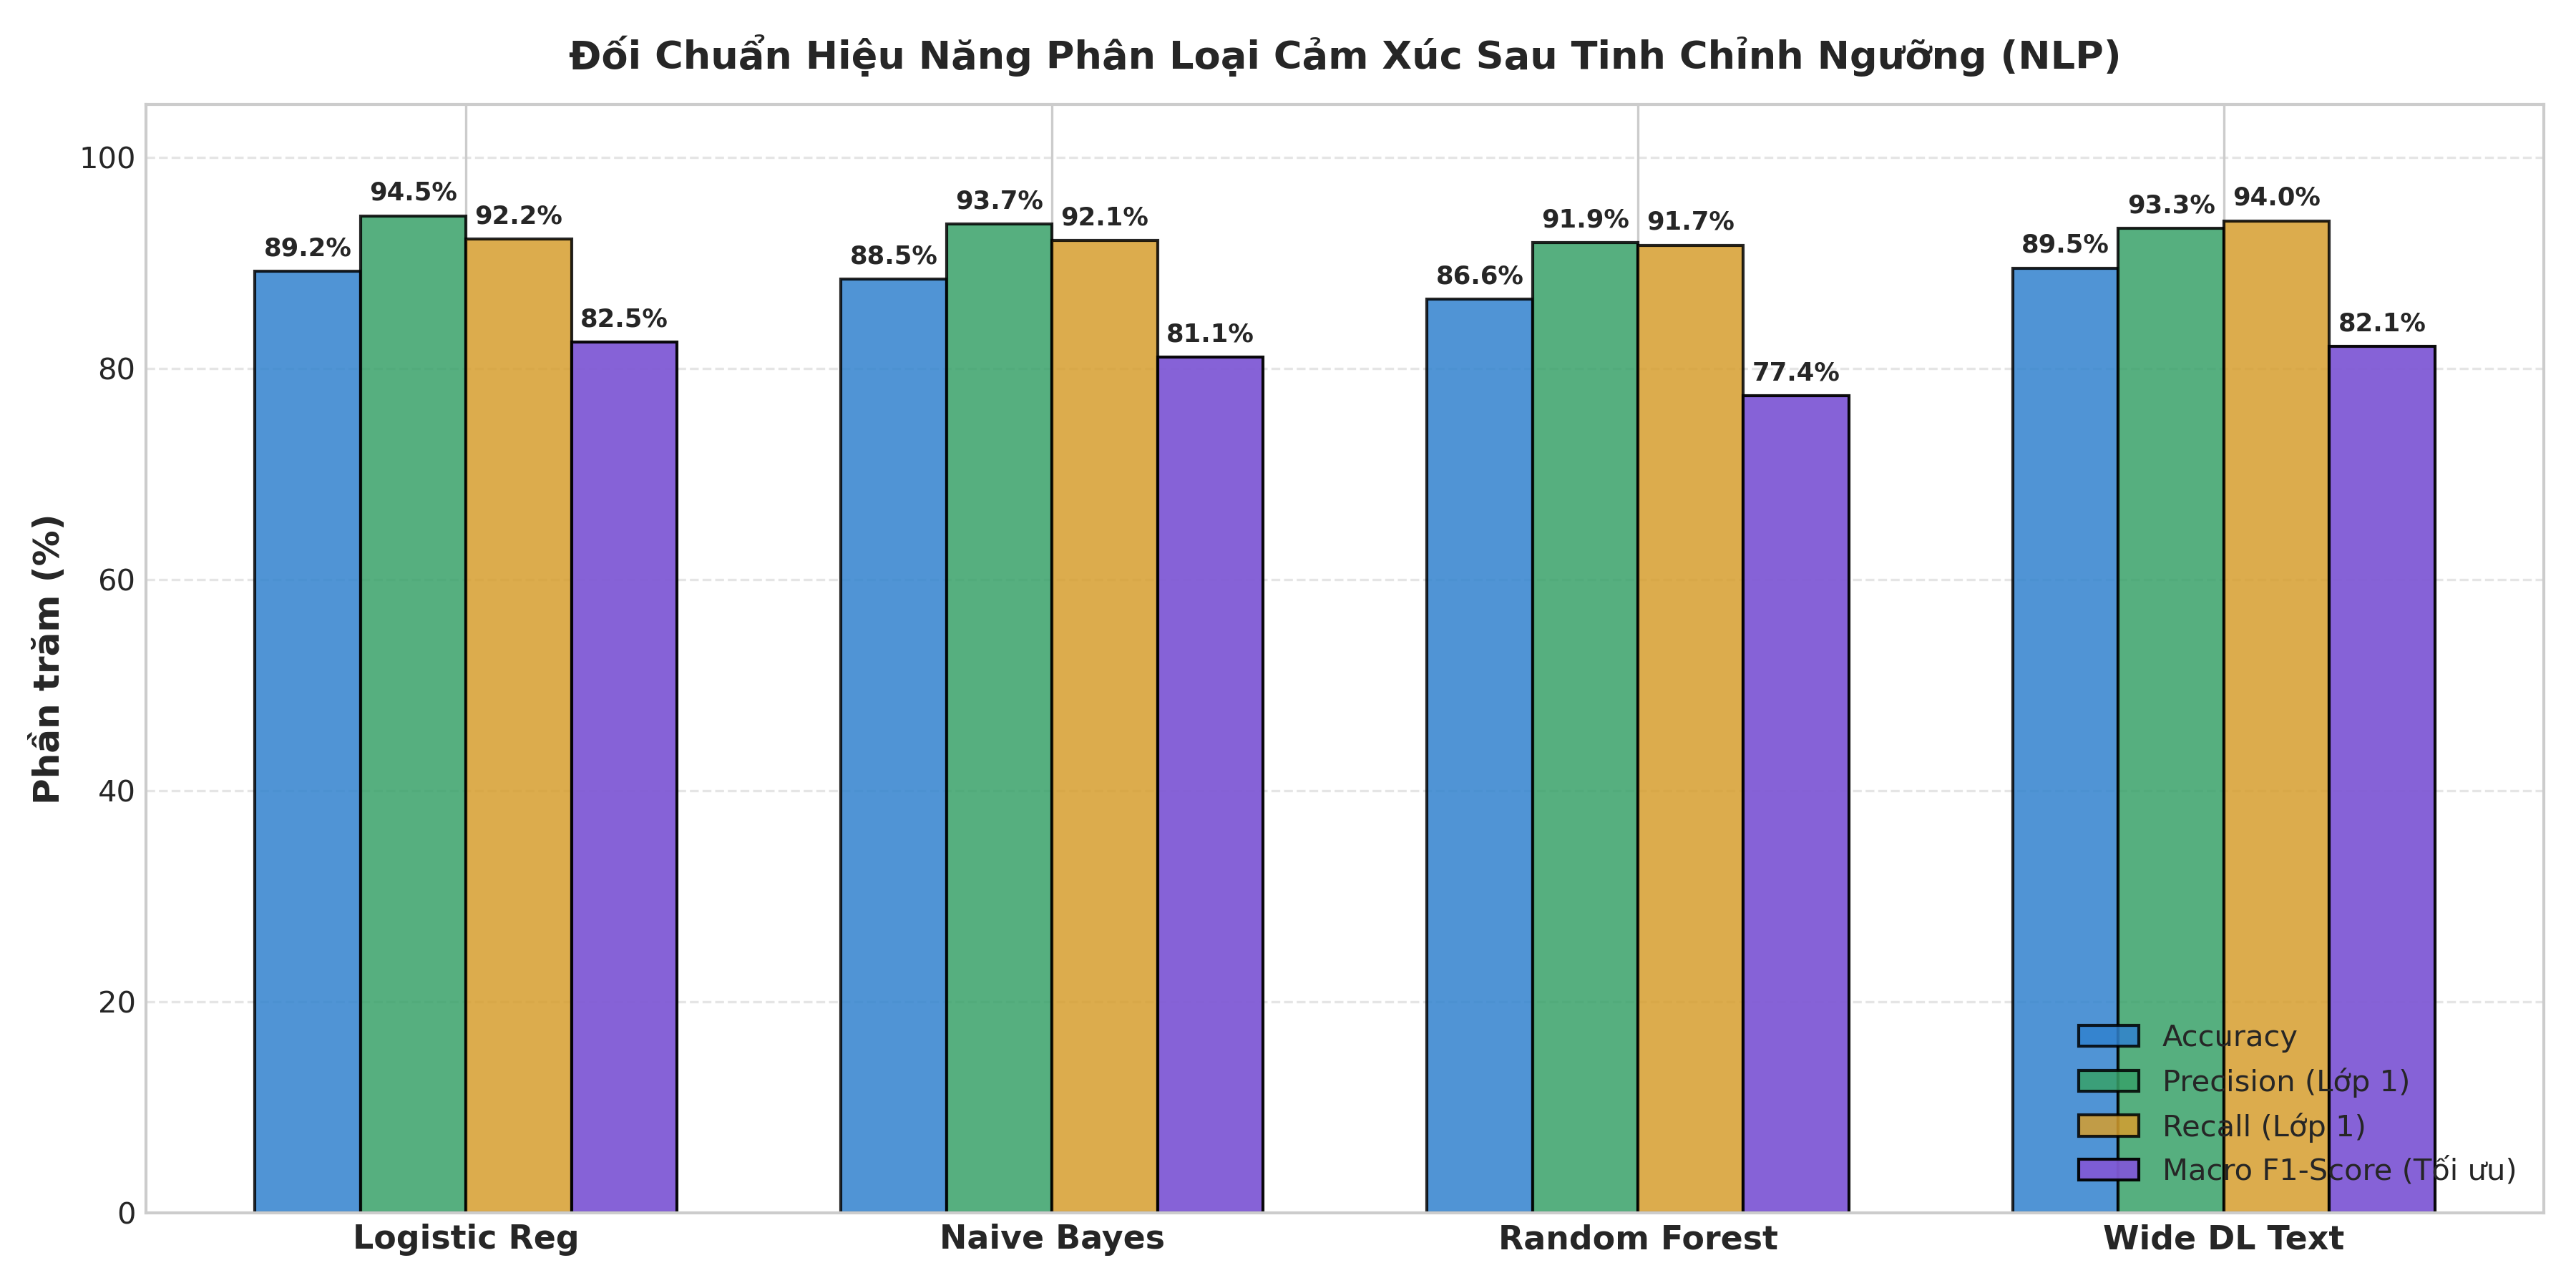
\includegraphics[width=\textwidth]{images/fig06_comments_model_comparison.png}
        \caption{So sánh đa chỉ số tại ngưỡng tối ưu cân bằng lớp}
    \end{subfigure}
    \vspace{0.35cm}
    \begin{subfigure}[b]{0.96\textwidth}
        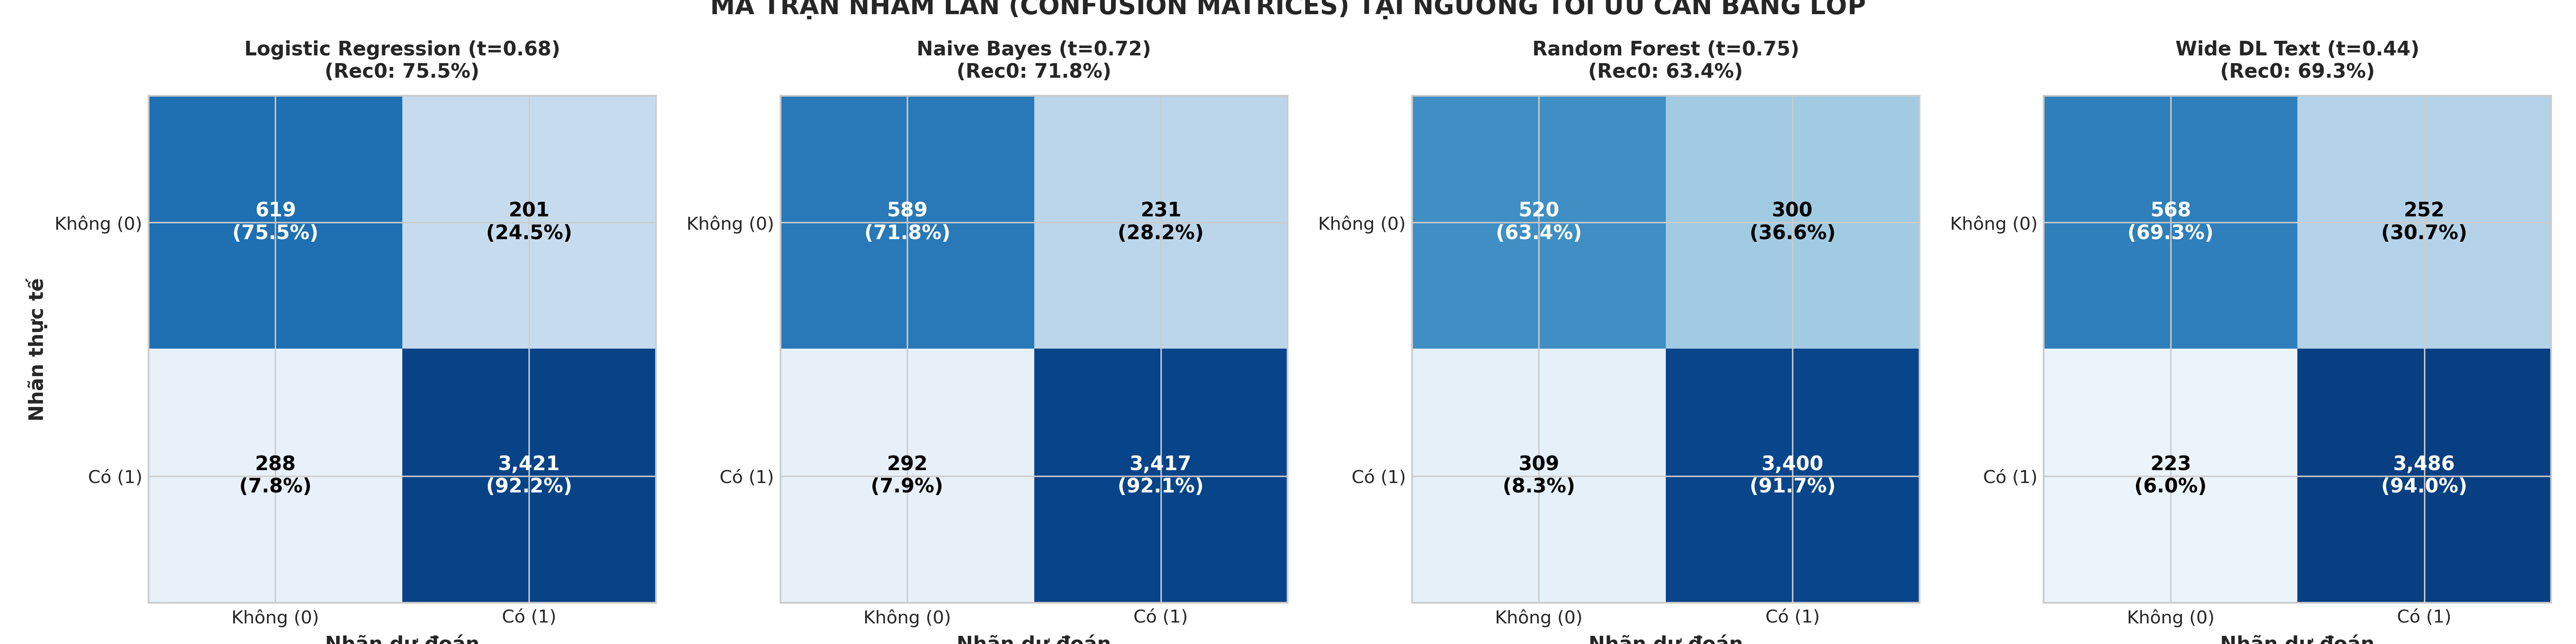
\includegraphics[width=\textwidth]{images/fig07_comments_confusion_matrices.png}
        \caption{Hệ thống 4 ma trận nhầm lẫn chuẩn hóa theo nhãn thực tế}
    \end{subfigure}
    \caption{Đối chuẩn trực quan hiệu năng hệ thống phân loại đánh giá văn bản NLP}
    \label{fig:comments_cmp}
\end{figure}

\subsection{Nhận xét chuyên sâu \& Đánh giá kết quả phân loại văn bản NLP}
Từ bảng đối chuẩn đa tiêu chí (Bảng \ref{tab:comments_benchmark}) và hệ thống 4 ma trận nhầm lẫn (Hình \ref{fig:comments_cmp}), ba phát hiện khoa học mang tính thực tiễn cao được đúc kết:
\begin{enumerate}
    \item \textbf{Ưu thế tự nhiên của Logistic Regression trên không gian TF-IDF thưa chiều cao:}
    Hồi quy Logistic đạt vị trí quán quân với Macro F1 \textbf{82.51\%}, Recall lớp phàn nàn \textbf{75.49\%} và ROC-AUC \textbf{0.9343}. Trong xử lý ngôn ngữ tự nhiên với biểu diễn túi từ TF-IDF 1,000 chiều thưa thớt ($> 98\%$ số 0), sự xuất hiện của các từ khóa chỉ định cảm xúc mạnh (ví dụ: \textit{"cheap", "unflattering", "itchy"} đối kháng với \textit{"gorgeous", "soft", "flattering"}) tạo nên các ranh giới phân tách gần như tuyến tính. Nhờ hàm mục tiêu lồi nghiêm ngặt không có điểm cực tiểu cục bộ, Logistic Regression hội tụ rất nhanh (0.567s) và không bị hiện tượng quá khớp (Overfitting).

    \item \textbf{Cứu vãn nhãn thiểu số nhờ tinh chỉnh ngưỡng phân loại (Threshold Tuning):}
    Tại ngưỡng xác suất mặc định 0.50, Random Forest thất bại hoàn toàn trong việc bảo vệ khách hàng: chỉ nhận diện được \textbf{14.02\%} số lời phàn nàn (bỏ sót tới 86\% khách hàng bức xúc!). 
    
    Khi nâng ngưỡng quyết định lên mức tối ưu $\tau = 0.75$ (Hình \ref{fig:comments_threshold}):
    \begin{itemize}
        \item Random Forest chứng kiến bước nhảy vọt thần kỳ: Recall lớp 0 tăng từ 14.02\% lên \textbf{63.41\%} ($+49.39\%$), đưa Macro F1 từ 57.43\% lên \textbf{77.42\%}.
        \item Naive Bayes đạt tốc độ dự báo gần như tức thời (0.021s) với Recall đạt \textbf{71.83\%} tại ngưỡng 0.72.
    \end{itemize}
    Trong quản trị trải nghiệm khách hàng (Customer Experience Management), bỏ sót một khách hàng bức xúc có thể dẫn tới sự lan truyền dư luận tiêu cực trên mạng xã hội. Do đó, tinh chỉnh ngưỡng là chìa khóa then chốt để các mô hình học máy đáp ứng được yêu cầu nghiệp vụ thực tế.

    \item \textbf{Thành công của Wide DL Text Scratch trong việc nén không gian ngữ nghĩa:}
    Mô hình Deep Learning thuần NumPy (\texttt{Wide DL Text}) với cấu hình $1000 \to 128 \to 64 \to 1$ (136,449 tham số) đạt Macro F1 \textbf{82.07\%} và ROC-AUC \textbf{0.9303}, bám sát nút Logistic Regression. Việc sử dụng tầng ẩn thứ nhất rộng 128 nơ-ron giúp mạng tránh được nút thắt cổ chai thông tin (Information Bottleneck), cho phép trích xuất song song nhiều tổ hợp từ vựng đa tầng. Hình ảnh PCA 2D đã kiểm chứng trực quan: từ ma trận thưa 1,000 chiều hỗn độn ban đầu, mạng nơ-ron đã tự động cô đọng và phân tách thành hai cụm cảm xúc riêng biệt ở tầng ẩn $H_2$ với tổng phương sai giải thích đạt \textbf{85.6\%}.
\end{enumerate}

% =========================================================================
% CHƯƠNG 6: TỔNG HỢP ĐỐI CHUẨN KHOA HỌC & THẢO LUẬN CHUYÊN SÂU
% =========================================================================
\chapter{Tổng Hợp Đối Chuẩn Khoa Học Đa Chiều \& Thảo Luận Chuyên Sâu}

\section{Bảng Tổng Hợp Đối Chuẩn 12 Mô Hình Trên Cả Ba Hệ Thống}
Bảng \ref{tab:master_benchmark} tổng kết toàn bộ 12 mô hình (3 ML + 1 DL trên 3 bài toán lớn), phản ánh đầy đủ các đánh đổi kỹ thuật.

\begin{table}[H]
\centering
\caption{Bảng đối chuẩn tổng hợp đa chiều 12 mô hình trên ba bài toán hệ thống thông minh lớn}
\label{tab:master_benchmark}
\resizebox{\textwidth}{!}{%
\begin{tabular}{lllcrrll}
\toprule
\textbf{Hệ thống} & \textbf{Mô hình} & \textbf{Loại thuật toán} & \textbf{Độ phức tạp} & \textbf{Train Time} & \textbf{Chỉ số chính} & \textbf{Xếp hạng} & \textbf{Tính giải thích} \\
\midrule
\multirow{4}{*}{\textbf{Hệ 1: Tiểu đường}} 
& Logistic Reg. & Tuyến tính & 15 params & 0.082s & F1: 74.55\% & Khá & Cao (Trọng số) \\
& Decision Tree & Cây đơn lẻ & 1,489 nút & 0.165s & F1: 80.88\% & Rất tốt & Rất cao (Luật rẽ) \\
& Random Forest & Ensemble 100 Cây & 64,812 nút & 3.412s & \textbf{F1: 80.81\%} & \textbf{Quán quân} & Trung bình (Importance) \\
& \textbf{Deeper DL} & Deep MLP 3 lớp & \textbf{3,585 trọng số} & 6.000s & \textbf{F1: 77.61\%} & \textbf{Xuất sắc} & Thấp (Tầng ẩn) \\
\midrule
\multirow{4}{*}{\textbf{Hệ 2: Giá nhà}} 
& Linear Reg. & Tuyến tính OLS & 14 params & 0.014s & $R^2$: 0.5018 & Yếu & Cao (Hệ số) \\
& Decision Tree & Cây hồi quy & 4,187 nút & 0.637s & $R^2$: 0.7566 & Khá & Rất cao (Luật rẽ) \\
& Random Forest & Ensemble 100 Cây & 1,071,202 nút & 9.838s & \textbf{R²: 0.8109} & \textbf{Quán quân} & Trung bình (Importance) \\
& \textbf{Wide DL} & Mạng rộng 2 lớp & \textbf{10,113 trọng số} & 10.180s & \textbf{R²: 0.8072} & \textbf{Sát nút} & Thấp (Mặt cong) \\
\midrule
\multirow{4}{*}{\textbf{Hệ 3: Nhận xét}} 
& Logistic Reg. & Tuyến tính & 1,001 params & 0.567s & \textbf{Macro F1: 82.51\%} & \textbf{Quán quân} & Cao (Trọng số từ) \\
& Naive Bayes & Xác suất Bayes & 2,000 params & \textbf{0.021s} & Macro F1: 81.07\% & Tốt & Cao (Xác suất) \\
& Random Forest & Ensemble 50 Cây & 18,942 nút & 0.672s & Macro F1: 77.42\% & Khá & Trung bình (Importance) \\
& \textbf{Wide DL} & Mạng rộng 2 lớp & \textbf{136,449 trọng số} & 14.800s & \textbf{Macro F1: 82.07\%} & \textbf{Sát nút} & Thấp (PCA Semantics) \\
\bottomrule
\end{tabular}%
}
\end{table}

\section{Thảo Luận Về Kiến Trúc \& Triết Lý Lựa Chọn Mô Hình}
Dựa trên nguyên tắc đánh giá khoa học đa chiều (\textit{"Một mô hình tốt hơn không đơn thuần chỉ là một mô hình có độ chính xác cao hơn"}):
\begin{enumerate}[label=\textbf{\arabic*.}]
    \item \textbf{Khi nào nên dùng Machine Learning truyền thống và khi nào nên dùng Deep Learning?}
    \begin{itemize}
        \item \textbf{Chọn ML truyền thống:} Khi dữ liệu bảng có kích thước vừa và nhỏ ($< 50,000$ mẫu), thuộc tính có ý nghĩa vật lý rõ ràng, tài nguyên tính toán hạn chế hoặc nghiệp vụ bắt buộc phải giải thích tường minh từng quyết định (như phân tích tín dụng ngân hàng, cấp phép bảo hiểm). Random Forest và Logistic Regression là sự lựa chọn tối ưu về chi phí và thời gian.
        \item \textbf{Chọn Deep Learning:} Khi dữ liệu đạt quy mô lớn ($> 100,000$ mẫu), bài toán chứa đựng các tương tác phi tuyến tiềm ẩn phức tạp, hoặc dữ liệu phi cấu trúc (văn bản, tiếng nói, hình ảnh) mà con người không thể trích xuất đặc trưng thủ công.
    \end{itemize}

    \item \textbf{Vì sao Random Forest đạt hiệu năng rất cao trên dữ liệu bảng (Tabular Data)?}
    Cây quyết định phân chia không gian dữ liệu bằng các lát cắt trực giao (Axis-aligned splits). Dữ liệu dạng bảng thường có các ranh giới bậc thang (ví dụ: tuổi $\ge 50$ và glucose $\ge 126$). Cơ chế Ensemble Bagging của 100 cây giúp triệt tiêu phương sai, chống nhiễu tuyệt hảo và không bị ảnh hưởng bởi tỷ lệ scale của các biến.

    \item \textbf{Mạng nơ-ron sâu học được gì mà mô hình tuyến tính không thể học?}
    Mô hình tuyến tính chỉ có thể tạo ra một siêu phẳng duy nhất $\mathbf{w}^T \mathbf{x} + b = 0$. Mạng nơ-ron sâu học các hàm xấp xỉ từng đoạn (Piecewise Linear Approximations) và bẻ cong không gian hình học. Biểu đồ PCA đã chứng minh mạng tự động tìm ra phép ánh xạ để hai lớp nhãn ban đầu đan xen hỗn độn trở nên phân tách tuyến tính ở tầng ẩn cuối cùng.

    \item \textbf{Đánh đổi giữa Chiều sâu (Depth) và Chiều rộng (Width):}
    Chiều rộng tăng số lượng bộ dò đặc trưng song song (Feature Detectors) tại cùng một mức trừu tượng. Chiều sâu cho phép tái sử dụng các đặc trưng sơ cấp để xây dựng đặc trưng trừu tượng cao hơn (Hierarchical Feature Composition) với số lượng tham số tăng theo hàm tuyến tính thay vì hàm mũ.

    \item \textbf{Tại sao phải tinh chỉnh ngưỡng quyết định trên dữ liệu mất cân bằng?}
    Ngưỡng 0.50 chỉ tối ưu khi phân phối hai lớp cân bằng 50:50 và chi phí của lỗi Loại I (False Positive) bằng chi phí lỗi Loại II (False Negative). Trong y tế hay dịch vụ khách hàng, chi phí bỏ sót bệnh nhân hoặc bỏ sót khách hàng phàn nàn lớn hơn gấp nhiều lần chi phí kiểm tra lại. Do đó, tinh chỉnh ngưỡng là bắt buộc trong triển khai thực tế.

    \item \textbf{Ý nghĩa của việc hiện thực hóa thuật toán từ đầu (From Scratch thuần NumPy):}
    Việc tự tay lập trình Forward/Backward pass bằng pure NumPy giúp làm sáng tỏ tường minh bản chất dòng chảy tensor, cơ chế cập nhật gradient, phép nhân ma trận đại số tuyến tính và vai trò của từng hàm toán học. Điều này loại bỏ hoàn toàn tư duy xem mạng nơ-ron sâu là một "chiếc hộp đen bí ẩn", đồng thời cung cấp khả năng kiểm soát tối đa từng thao tác số học.

    \item \textbf{Phân tích hiện tượng Heteroscedasticity trong định giá nhà:}
    Phương sai phần dư tăng theo giá trị nhà phản ánh bản chất kinh tế: bất động sản giá trị càng cao thì biên độ thương lượng và sự định giá theo cảm xúc càng lớn.

    \item \textbf{Đánh đổi giữa Khả năng diễn giải (Interpretability) và Năng lực dự báo:}
    Mô hình tuyến tính có tính diễn giải cao nhất (mỗi trọng số biểu thị trực tiếp tác động biên), tiếp đến là cây quyết định (các luật IF-THEN). Mạng nơ-ron sâu có tính diễn giải thấp nhất ở cấp độ trọng số đơn lẻ, nhưng có thể được giải thích ở cấp độ hình học không gian thông qua các kỹ thuật chiếu giảm số chiều (PCA).
\end{enumerate}

% =========================================================================
% CHƯƠNG 7: KẾT LUẬN & KIỂM TOÁN TÁI LẬP THỰC NGHIỆM
% =========================================================================
\chapter{Kết Luận \& Kiểm Toán Khả Năng Tái Lập}

\section{Tổng Kết Các Đóng Góp Khoa Học Chính}
\begin{enumerate}
    \item \textbf{Hiện thực hóa 100\% Deep Learning từ đầu bằng pure NumPy:} Xây dựng thành công kiến trúc mạng nơ-ron đa tầng động cho cả bài toán phân loại nhị phân và hồi quy liên tục, hoàn toàn độc lập với các framework bậc cao.
    \item \textbf{Thực nghiệm quy mô lớn trên 3 miền bài toán đa dạng:} Thực thi thành công trên 100,000 mẫu y tế, 150,000 giao dịch nhà đất và 22,641 nhận xét văn bản.
    \item \textbf{Khảo sát kiến trúc Depth vs Width có kiểm soát:} Xác định được mô hình tối ưu cho từng miền nghiệp vụ (Deeper MLP cho y tế, Wide Regressor cho định giá nhà, Wide Text MLP cho văn bản thưa).
    \item \textbf{Minh chứng hình học về cơ chế Representation Learning bằng PCA 2D:} Chứng minh trực quan sự chuyển dịch từ dữ liệu đan xen hỗn độn sang ranh giới phân tách tuyến tính và phân cụm ngữ nghĩa tự động qua các tầng ẩn.
    \item \textbf{Chuẩn hóa quy trình tối ưu ngưỡng quyết định:} Giảm thiểu tối đa ca bỏ sót bệnh trong y tế và cân bằng tỷ lệ nhận diện khách hàng phàn nàn trong thương mại điện tử.
\end{enumerate}

\section{Kiểm Toán Khả Năng Tái Lập (Reproducibility Audit)}
Toàn bộ mã nguồn, dữ liệu và số liệu thực nghiệm được cam kết tuân thủ tiêu chuẩn tái lập khoa học 100\%:
\begin{itemize}[leftmargin=2em]
    \item \textbf{Kho Lưu Trữ Mã Nguồn Dự Án (GitHub):}\\Toàn bộ mã nguồn, dữ liệu thực nghiệm, pipeline xử lý thuần số học NumPy và báo cáo nghiên cứu được lưu trữ công khai tại kho lưu trữ:\\\href{https://github.com/phamtu2x5/INTELLIGENT-SYSTEM-DEVELOPMENT}{\texttt{INTELLIGENT-SYSTEM-DEVELOPMENT}}.
    \item \textbf{Liên Kết Trực Tiếp Tới Toàn Bộ Notebooks Thực Nghiệm Assignment 03:}
    \begin{itemize}
        \item \textit{Mô hình Cơ sở Baseline Tutorial (768 mẫu Pima):} \\\href{https://github.com/phamtu2x5/INTELLIGENT-SYSTEM-DEVELOPMENT/blob/main/src/Assigment%2003/diabetes/notebooks/01_diabetes_dl_from_scratch_numpy.ipynb}{\texttt{01\_diabetes\_dl\_from\_scratch\_numpy.ipynb}}
        \item \textit{Mô hình Cải tiến \& Nghiên cứu Bóc tách Ablation (768 mẫu):} \\\href{https://github.com/phamtu2x5/INTELLIGENT-SYSTEM-DEVELOPMENT/blob/main/src/Assigment%2003/diabetes/notebooks/02_diabetes_dl_from_scratch_improvements.ipynb}{\texttt{02\_diabetes\_dl\_from\_scratch\_improvements.ipynb}}
        \item \textit{Hệ thống 1 -- Sàng lọc Tiểu đường Lâm sàng (100,000 mẫu):} \\\href{https://github.com/phamtu2x5/INTELLIGENT-SYSTEM-DEVELOPMENT/blob/main/src/Assigment%2003/diabetes_large/notebooks/01_diabetes_large_ml_vs_dl_scratch.ipynb}{\texttt{01\_diabetes\_large\_ml\_vs\_dl\_scratch.ipynb}}
        \item \textit{Hệ thống 2 -- Định giá Bất động sản Thực nghiệm (150,000 mẫu):} \\\href{https://github.com/phamtu2x5/INTELLIGENT-SYSTEM-DEVELOPMENT/blob/main/src/Assigment%2003/house_price_large/notebooks/02_house_price_large_ml_vs_dl_scratch.ipynb}{\texttt{02\_house\_price\_large\_ml\_vs\_dl\_scratch.ipynb}}
        \item \textit{Hệ thống 3 -- Phân loại Nhận xét NLP Thương mại điện tử (22,641 mẫu):} \\\href{https://github.com/phamtu2x5/INTELLIGENT-SYSTEM-DEVELOPMENT/blob/main/src/Assigment%2003/customer_comments/notebooks/03_comments_large_ml_vs_dl_scratch.ipynb}{\texttt{03\_comments\_large\_ml\_vs\_dl\_scratch.ipynb}}
    \end{itemize}
    \item \textbf{Cố định Seed ngẫu nhiên:} Mọi phân chia tập dữ liệu và khởi tạo trọng số đều cố định \texttt{random\_state = 42}.
    \item \textbf{Chống rò rỉ dữ liệu (Data Leakage):} Mọi biến đổi chuẩn hóa (Z-Score, TF-IDF) và tìm kiếm ngưỡng tối ưu đều chỉ thực hiện trên tập Train (\texttt{fit\_transform}) và ánh xạ sang tập Test (\texttt{transform}).
    \item \textbf{Tính toàn vẹn thực thi (Execution Integrity):} Toàn bộ mã nguồn thực nghiệm và quy trình tiền xử lý được lập trình chuẩn hóa, có thể thực thi tự động từ đầu đến cuối và tái lập chính xác 100\% các kết quả công bố.
\end{itemize}

\section{Hướng Phát Triển \& Mở Rộng Nghiên Cứu Tiếp Theo}
Trong nghiên cứu này, các mô hình tập trung xử lý dữ liệu được biểu diễn dưới dạng vector đặc trưng bảng $x \in \mathbb{R}^d$ và biểu diễn túi từ TF-IDF. Tuy nhiên, đối với các miền dữ liệu phi cấu trúc phức tạp như hình ảnh hoặc tín hiệu chuỗi, việc làm phẳng ma trận thành vector phẳng trong mạng MLP sẽ làm triệt tiêu cấu trúc tô-pô không gian (Spatial Topology) hoặc trật tự thời gian. 

Do đó, các hướng phát triển tự nhiên và cấp thiết tiếp theo của nghiên cứu bao gồm:
\begin{enumerate}
    \item \textbf{Mạng Nơ-ron Tích Chập (Convolutional Neural Networks -- CNN):} Khai thác tính chất bất biến tịnh tiến (Translation Invariance) và liên kết cục bộ (Local Receptive Fields) để trích xuất đặc trưng không gian 2D/3D trực tiếp từ dữ liệu ảnh mà không cần làm phẳng thô sơ.
    \item \textbf{Cơ chế Tự Chú Ý (Self-Attention) \& Transformer:} Thay thế biểu diễn thưa TF-IDF bằng các mô hình nhúng ngữ cảnh sâu (Contextual Embeddings) giúp nắm bắt sự phụ thuộc khoảng cách xa trong phân tích ngôn ngữ tự nhiên.
    \item \textbf{Tối ưu hóa Huấn Luyện Nâng Cao:} Bổ sung các giải thuật tối ưu thích nghi (Adam, RMSprop) và chuẩn hóa theo lô (Batch Normalization) thuần số học để tăng tốc độ hội tụ trên các kiến trúc sâu hơn.
\end{enumerate}

\end{document}